% !TeX document-id = {c6282027-a510-40f1-b05e-2f558a6cd3f1}
% !TeX program = xelatex
% !TeX TXS-program:compile = txs:///xelatex/[--shell-escape]
%%%%%%%%%%%%%%%%%%%%%%%%%%%%%%%%%%%%%%%%%%%%%%%%%%%%%%%%%%%%%%%%%%%%%%%%
% Plantilla para escribir libros
% Universidad de A Coruña. Facultad de Informática
% Realizado por: Welton Vieira dos Santos
% Modificado: Welton Vieira dos Santos
% Contacto: welton.dosssantos@udc.es
%%%%%%%%%%%%%%%%%%%%%%%%%%%%%%%%%%%%%%%%%%%%%%%%%%%%%%%%%%%%%%%%%%%%%%%%


% Archivo .TEX que incluye todas las configuraciones del documento y los paquetes. Añade todo aquello que necesites utilizar en el documento en este archivo.
% En él se encuentra la configuración de los márgenes, establecidos según las directrices de estilo de la EPS.
%%%%%%%%%%%%%%%%%%%%%%%%%%%%%%%%%%%%%%%%%%%%%%%%%%%%%%%%%%%%%%%%%%%%%%%%
% Plantilla para escribir libros
% Universidad de A Coruña. Facultad de Informática
% Realizado por: Welton Vieira dos Santos
% Modificado: Welton Vieira dos Santos
% Contacto: welton.dosssantos@udc.es
%%%%%%%%%%%%%%%%%%%%%%%%%%%%%%%%%%%%%%%%%%%%%%%%%%%%%%%%%%%%%%%%%%%%%%%%


%%%%%%%%%%%%%%%%%%%%%%%%
% FORMATO DEL DOCUMENTO
%%%%%%%%%%%%%%%%%%%%%%%%
% scrbook es la clase de documento
% Si se desea que no haya página en blanco entre capítulos añadir "openany" en los parámetros de la clase. Sino siempre los capítulos empezarán en página impar.
\documentclass[a4paper,12pt,titlepage]{scrbook}
\KOMAoption{toc}{bib,chapterentryfill} % Opciones del índice
\usepackage{scrhack} % Previene algunos errores
% Paquete de formato para scrbook. Con marcas, linea-separador superior e inferior
\usepackage[automark,headsepline,footsepline]{scrlayer-scrpage}
\clearpairofpagestyles		% Borra los estilos por defecto
%%
% Formato y contenido de la información de cabecera y pie de página
%%
% Información de capítulo en cabecera e interno
\ihead{{\color{gray30}\scshape\small\headmark}}	
% Número de página en cabecera y externo
\ohead{\normalfont\pagemark} 
% Número de página en pie de página y externo. Sólo en páginas sin cabecera
%\ofoot[\normalfont\pagemark]{}
%% 		
% Edición del contenido de las distintas partes de la cabecera
%%
\renewcommand{\chaptermark}[1]{\markboth{#1}{}} % Capítulo (Solo texto)
\renewcommand{\sectionmark}[1]{\markright{\thesection. #1}} % Sección (Número y texto)
\setkomafont{pagenumber}{} % Número de página (Sin nada añadido)

% Añade al índice y numera hasta la profundidad 4.
% 1:section,2:subsection,3:subsubsection,4:paragraph
\setcounter{tocdepth}{2}
\setcounter{secnumdepth}{2}
% Muestra una regla para comprobar el formato de las páginas
%\usepackage[type=upperleft,showframe,marklength=8mm]{fgruler}
% MÁRGENES DE LAS PÁGINAS
\usepackage[
  inner	=	3.0cm, % Margen interior
  outer	=	2.5cm, % Margen exterior
  top	=	2.5cm, % Margen superior
  bottom=	2.5cm, % Margen inferior
  includeheadfoot, % Incluye cabecera y pie de página en los márgenes
]{geometry}
% Valor de interlineado
\renewcommand{\baselinestretch}{1.0} % 1 línea de interlineado
% Para poder generar páginas horizontales
\usepackage{lscape}
% Ancho de la zona para comentarios en el margen. (modificado para todonotes)
\setlength{\marginparwidth}{1.9cm}

%%%%%%%%%%%%%%%%%%%%%%%%
% BIBLIOGRAFÍA
%%%%%%%%%%%%%%%%%%%%%%%%
%\usepackage{apacite} % NORMA APA
\usepackage[numbers,sort]{natbib}
\usepackage{breakcites}

%%%%%%%%%%%%%%%%%%%%%%%%
% DOCUMENTO EN ESPAÑOL
%%%%%%%%%%%%%%%%%%%%%%%%
\usepackage[base]{babel}
\usepackage{polyglossia}
\setdefaultlanguage{spanish}

\addto\captionsspanish{%
	\renewcommand{\listtablename}{Índice de tablas} 
	\renewcommand{\tablename}{Tabla}
	\renewcommand{\lstlistingname}{Código}
	\renewcommand{\lstlistlistingname}{Índice de \lstlistingname s}
	\renewcommand{\glossaryname}{Glosario}
	\renewcommand{\acronymname}{Acrónimos}
	\renewcommand{\bibname}{Bibliografía}%
}

%%%%%%%%%%%%%%%%%%%%%%%% 
% COLORES
%%%%%%%%%%%%%%%%%%%%%%%% 
% Biblioteca de colores
\usepackage{color}
\usepackage[dvipsnames]{xcolor}
% Otros colores definidos por el usuario
\definecolor{gray97}{gray}{.97}
\definecolor{gray75}{gray}{.75}
\definecolor{gray45}{gray}{.45}
\definecolor{gray30}{gray}{.30}
\definecolor{negro}{RGB}{0,0,0}
\definecolor{blanco}{RGB}{255,255,255}
\definecolor{dkgreen}{rgb}{0,.6,0}
\definecolor{dkblue}{rgb}{0,0,.6}
\definecolor{dkyellow}{cmyk}{0,0,.8,.3}
\definecolor{gray}{rgb}{0.5,0.5,0.5}
\definecolor{mauve}{rgb}{0.58,0,0.82}
\definecolor{deepblue}{rgb}{0,0,0.5}
\definecolor{deepred}{rgb}{0.6,0,0}
\definecolor{deepgreen}{rgb}{0,0.5,0}
\definecolor{MyDarkGreen}{rgb}{0.0,0.4,0.0}
\definecolor{bluekeywords}{rgb}{0.13,0.13,1}
\definecolor{greencomments}{rgb}{0,0.5,0}
\definecolor{redstrings}{rgb}{0.9,0,0}

%%%%%%%%%%%%%%%%%%%%%%%%
% TABLAS
%%%%%%%%%%%%%%%%%%%%%%%%
% Paquetes para tablas
\usepackage{longtable,booktabs,array,multirow,tabularx,ragged2e,array}
% Nuevos tipos de columna para tabla, se pueden utilizar como por ejemplo C{3cm} en la definición de columnas de la función tabular
\newcolumntype{L}[1]{>{\raggedright\let\newline\\\arraybackslash\hspace{0pt}}m{#1}}
\newcolumntype{C}[1]{>{\centering\let\newline\\\arraybackslash\hspace{0pt}}m{#1}}
\newcolumntype{R}[1]{>{\raggedleft\let\newline\\\arraybackslash\hspace{0pt}}m{#1}}

%%%%%%%%%%%%%%%%%%%%%%%% 
% GRAFICAS y DIAGRAMAS 
%%%%%%%%%%%%%%%%%%%%%%%% 
% Paquete para todo tipo de gráficas, diagramas, modificación de imágenes, etc
\usepackage{tikz,tikzpagenodes}
\usetikzlibrary{tikzmark,calc,shapes.geometric,arrows,backgrounds,shadings,shapes.arrows,shapes.symbols,shadows,positioning,fit,automata}
\usepackage{pgfplots}
\pgfplotsset{compat=newest} % Compatibilidad
\usepackage{pgfplotstable}
% Estilos para elementos graficos
% Cajas y cajas de texto
\tikzstyle{Caja1} = [green,very thick,rounded corners,fill=white, fill opacity=0.5]
\tikzstyle{Texto1} = [fill=white,thick,shape=circle,draw=black,inner sep=2pt,font=\sffamily,text=black]
\tikzstyle{Texto2} = [fill=white,thick,shape=rectangle,draw=black,inner sep=2pt,font=\sffamily,text=black]
\tikzstyle{Texto3} = [fill=white,thick,shape=circle,draw=black,inner sep=2pt,font=\sffamily,text=black]
% Cuadros de diagrama
\tikzstyle{rectvioleta} = [rectangle, rounded corners, text centered, draw=black, fill=blue!10]
\tikzstyle{rectnaranja} = [rectangle, minimum width=2cm, minimum height=1cm, text centered, draw=black, fill=orange!10]
\tikzstyle{romborosa} = [diamond, aspect=3, minimum width=3cm, minimum height=1cm, text centered, draw=black, fill=red!10]
\tikzstyle{rectverde} = [rectangle, minimum width=2cm, minimum height=1cm, text centered, draw=black, fill=green!10]
\tikzstyle{rectamarillo} = [rectangle, rounded corners, minimum width=2cm, minimum height=1cm, text centered, draw=black, fill=yellow!10]
% Flechas
\tikzstyle{arrow} = [thick,->,>=stealth]

%%%%%%%%%%%%%%%%%%%%%%%% 
% FIGURAS, TABLAS, ETC 
%%%%%%%%%%%%%%%%%%%%%%%% 
\usepackage{subcaption} % Para poder realizar subfiguras
\usepackage{caption} % Para aumentar las opciones de diseño
% Nombres de figuras, tablas, etc, en negrita la numeración, todo con letra small
\captionsetup{labelfont={bf,small},textfont=small}
% Paquete para modificar los espacios arriba y abajo de una figura o tabla
\usepackage{setspace}
% Define el espacio tanto arriba como abajo de las figuras, tablas
\setlength{\intextsep}{5mm}
% Para ajustar tamaños de texto de toda una tabla o grafica
% Uso: {\scalefont{0.8} \begin{...} \end{...} }
\usepackage{scalefnt}
% Redefine las tablas y figuras para eliminar el '.' entre la numeración y el texto
\renewcommand*{\figureformat}{\figurename~\thefigure}
\renewcommand*{\tableformat}{\tablename~\thetable}

%%%%%%%%%%%%%%%%%%%%%%%% 
% TEXTO
%%%%%%%%%%%%%%%%%%%%%%%%
% Paquete para poder modificar las fuente de texto
\usepackage{xltxtra}
% Cualquier tamaño de texto. Uso: {\fontsize{100pt}{120pt}\selectfont tutexto}
\usepackage{anyfontsize}
% Para modificar parametros del texto.
\usepackage{setspace}
% Paquete para posicionar bloques de texto
\usepackage{textpos}
% Paquete para realizar cajas de texto. 
% Uso: \begin{mdframed}[linecolor=red!100!black] tutexto \end{mdframed}
\usepackage{framed,mdframed}
% Para subrayar. Uso: \hlc[tucolor]{tutexto}
\newcommand{\hlc}[2][yellow]{ {\sethlcolor{#1} \hl{#2}} }
% Para que el salto de linea funcione sin tener que usar \\
%\usepackage{parskip}

%%%%%%%%%%%%%%%%%%%%%%%% 
% OTROS
%%%%%%%%%%%%%%%%%%%%%%%%
% Para hacer una pagina horizontal. Uso: \begin{landscape} xxxx \end{lanscape}
\usepackage{lscape} 
% Para incluir paginas PDF. Uso:
% \includepdf[pages={1}]{tuarchivo.pdf}
\usepackage{pdfpages}
% Para introducir url's con formato. Uso: \url{http://www.google.es}
\usepackage{url}
% Amplia muchas funciones graficas de latex
\usepackage{graphicx}
\graphicspath{ {archivos/images/} }
% Paquete que añade el hipervinculo en referencias dentro del documento, indice, etc
% Se define sin bordes alrededor. Uso: \ref{tulabel}
\usepackage[pdfborder={000}]{hyperref}
\usepackage{float}
\usepackage{placeins}
\usepackage{afterpage}
\usepackage{verbatim}
% Paquete para condicionales avanzados
\usepackage{xstring,xifthen}
% Paquete para realizar calculos en el código
\usepackage{calc}
% Para incluir comentrios en el texto. El parámetro 'disable' oculta todas las notas.
% USO: \todo{tutexto}
\usepackage[textsize=tiny,spanish,shadow,textwidth=2cm]{todonotes}
%\reversemarginpar % Descomentar si se quiere todos los comentarios en el mismo lado

%%%%%%%%%%%%%%%%%%%%%%%% 
% GLOSARIOS
%%%%%%%%%%%%%%%%%%%%%%%%
\usepackage[acronym,nonumberlist,toc]{glossaries}
\usepackage{glossary-superragged}
\newglossarystyle{modsuper}{%
  \setglossarystyle{super}%
  \renewcommand{\glsgroupskip}{}
}
\renewcommand{\glsnamefont}[1]{\textbf{#1}}


%%%%%%%%%%%%%%%%%%%%%%%% 
% COMANDOS AÑADIDOS
%%%%%%%%%%%%%%%%%%%%%%%%
% Para mostrar la fecha actual (mes año) con \Hoy
\newcommand{\DIA}{\number\day \space}
\newcommand{\MES}{%
  \ifcase\month% 0
    \or Enero% 1
    \or Febrero% 2
    \or Marzo% 3
    \or Abril% 4
    \or Mayo% 5
    \or Junio% 6
    \or Julio% 7
    \or Agosto% 8
    \or Septiembre% 9
    \or Octubre% 10
    \or Noviembre% 11
    \or Diciembre% 12
  \fi}
\newcommand{\ANYO}{\number\year}
\newcommand{\Hoy}{\DIA de \MES\ de \ANYO}

%%%%%%%%%%%%%%%%%%%%%%%% 
% MATEMÁTICAS
%%%%%%%%%%%%%%%%%%%%%%%%
\RequirePackage{mathtools,amsthm,amsfonts,amssymb,bm,mathrsfs} 
\RequirePackage{upgreek}
% Comando para añadir información de variables a las ecuaciones
% Uso: \begin{condiciones}[donde:] ....... \end{condiciones}
\newenvironment{condiciones}[1][2]
  {%
   #1\tabularx{\textwidth-\widthof{#1}}[t]{
     >{$}l<{$} @{}>{${}}c<{{}$}@{} >{\raggedright\arraybackslash}X
   }%
  }
  {\endtabularx\\[\belowdisplayskip]}

%%%%%
% PARÁMETROS DE FORMATO DE CODIGOS
%%%%%
% Puedes editar los formatos para ajustarlos a tu gusto
%%%%%%%%%%%%%%%%%%%%%%%%%%%%%%%%%%%%%%%%%%%%%%%%%%%%%%%%%%%%%%%%%%%%%%%%
% Plantilla para escribir libros
% Universidad de A Coruña. Facultad de Informática
% Realizado por: Welton Vieira dos Santos
% Modificado: Welton Vieira dos Santos
% Contacto: welton.dosssantos@udc.es
%%%%%%%%%%%%%%%%%%%%%%%%%%%%%%%%%%%%%%%%%%%%%%%%%%%%%%%%%%%%%%%%%%%%%%%%


%%%%%%%%%%%%%%%%%%%%%%%% 
% CÓDIGO. CONFIGURACIÓN. En el siguiente bloque están los estilos.
%%%%%%%%%%%%%%%%%%%%%%%%
% Paquete para mostrar código de matlab. En caja y lineas numeradas
\usepackage[framed,numbered]{matlab-prettifier}
% Paquete mostrar código de programación de distintos lenguajes
\usepackage{listings}
\lstset{ inputencoding=utf8,
extendedchars=true,
frame=single, % Caja donde se ubica el código
backgroundcolor=\color{gray97}, % Color del fondo de la caja
rulesepcolor=\color{black},
boxpos=c,
abovecaptionskip=-4pt,
aboveskip=12pt,
belowskip=0pt,
lineskip=0pt,
framerule=0pt,
framextopmargin=4pt,
framexbottommargin=4pt,
framexleftmargin=11pt,
framexrightmargin=0pt,
linewidth=\linewidth,
xleftmargin=\parindent,
framesep=0pt,
rulesep=.4pt,
stringstyle=\ttfamily,
showstringspaces = false,
showspaces = false,
showtabs = false,
columns=fullflexible,
basicstyle=\small\ttfamily,
commentstyle=\color{gray45},
keywordstyle=\bfseries,
tabsize=4,
numbers=left,
numbersep=1pt,
numberstyle=\tiny\ttfamily\color{gray75},
numberfirstline = false,
breaklines=true,
postbreak=\mbox{\textcolor{red}{$\hookrightarrow$}\space}, % Flecha al saltar de linea
prebreak=\mbox{\textcolor{red}{$\hookleftarrow$}\space}, % Flecha al saltar de linea
literate=
  {á}{{\'a}}1 {é}{{\'e}}1 {í}{{\'i}}1 {ó}{{\'o}}1 {ú}{{\'u}}1
  {Á}{{\'A}}1 {É}{{\'E}}1 {Í}{{\'I}}1 {Ó}{{\'O}}1 {Ú}{{\'U}}1
  {à}{{\`a}}1 {è}{{\`e}}1 {ì}{{\`i}}1 {ò}{{\`o}}1 {ù}{{\`u}}1
  {À}{{\`A}}1 {È}{{\'E}}1 {Ì}{{\`I}}1 {Ò}{{\`O}}1 {Ù}{{\`U}}1
  {ä}{{\"a}}1 {ë}{{\"e}}1 {ï}{{\"i}}1 {ö}{{\"o}}1 {ü}{{\"u}}1
  {Ä}{{\"A}}1 {Ë}{{\"E}}1 {Ï}{{\"I}}1 {Ö}{{\"O}}1 {Ü}{{\"U}}1
  {â}{{\^a}}1 {ê}{{\^e}}1 {î}{{\^i}}1 {ô}{{\^o}}1 {û}{{\^u}}1
  {Â}{{\^A}}1 {Ê}{{\^E}}1 {Î}{{\^I}}1 {Ô}{{\^O}}1 {Û}{{\^U}}1
  {œ}{{\oe}}1 {Œ}{{\OE}}1 {æ}{{\ae}}1 {Æ}{{\AE}}1 {ß}{{\ss}}1
  {ű}{{\H{u}}}1 {Ű}{{\H{U}}}1 {ő}{{\H{o}}}1 {Ő}{{\H{O}}}1
  {ç}{{\c c}}1 {Ç}{{\c C}}1 {ø}{{\o}}1 {å}{{\r a}}1 {Å}{{\r A}}1
  {€}{{\euro}}1 {£}{{\pounds}}1 {«}{{\guillemotleft}}1
  {»}{{\guillemotright}}1 {ñ}{{\~n}}1 {Ñ}{{\~N}}1 {¿}{{?`}}1,
  }

% Intenta no dividir los códigos en diferentes paginas si es posible
\lstnewenvironment{listing}[1][]
   {\lstset{#1}\pagebreak[0]}{\pagebreak[0]}

% Formato de títulos de los códigos
\DeclareCaptionFont{white}{\color{white}}
\DeclareCaptionFormat{listing}{\colorbox{gray}{\parbox{\textwidth - 2\fboxsep}{#1#2#3}}}
\captionsetup[lstlisting]{format=listing,labelfont=white,textfont=white,font= scriptsize}


%%%%%%%%%%%%%%%%%%%%%%%% 
% CÓDIGO. ESTILOS. Ajústalos a tu gusto
%%%%%%%%%%%%%%%%%%%%%%%%
\lstdefinestyle{Consola}
	{
	basicstyle=\scriptsize\bf\ttfamily,
	}
   
\lstdefinestyle{C}
	{
	basicstyle=\scriptsize,
	language=C,
	}
\lstdefinestyle{C-color}
	{
  	breaklines=true,
  	language=C,
  	basicstyle=\scriptsize,
  	keywordstyle=\bfseries\color{green!40!black},
  	commentstyle=\itshape\color{purple!40!black},
  	identifierstyle=\color{blue},
  	stringstyle=\color{orange},
    }
\lstdefinestyle{CSharp}
	{
	basicstyle=\scriptsize
	language=[Sharp]C,
	escapeinside={(*@}{@*)},
	keywordstyle=\bfseries,
	}
\lstdefinestyle{CSharp-color}
	{
	basicstyle=\scriptsize
	language=[Sharp]C,
	escapeinside={(*@}{@*)},
	commentstyle=\color{greencomments},
	keywordstyle=\color{bluekeywords}\bfseries,
	stringstyle=\color{redstrings},
	}
\lstdefinestyle{C++}
	{
	basicstyle=\scriptsize,
	language=C++,
 	}
 	
\lstdefinestyle{C++-color}
	{
  	breaklines=true,
  	language=C++,
  	basicstyle=\scriptsize,
  	keywordstyle=\bfseries\color{green!40!black},
  	commentstyle=\itshape\color{purple!40!black},
  	identifierstyle=\color{blue},
  	stringstyle=\color{orange},
    }
    
\lstdefinestyle{PHP}
	{
	basicstyle=\scriptsize,
	language=PHP,
	}
	
\lstdefinestyle{PHP-color}
	{
	basicstyle=\scriptsize,
	language=PHP,
	keywordstyle    = \color{dkblue},
  	stringstyle     = \color{red},
  	identifierstyle = \color{dkgreen},
  	commentstyle    = \color{gray},
  	emph            =[1]{php},
  	emphstyle       =[1]\color{black},
  	emph            =[2]{if,and,or,else},
  	emphstyle       =[2]\color{dkyellow}
  }
  
\lstdefinestyle{Matlab}
	{
	basicstyle=\scriptsize,
	language=Matlab,
	numberstyle=\tiny\ttfamily\color{gray75},
	}
	
\lstdefinestyle{Matlab-color}
	{
	style = Matlab-editor,
	basicstyle=\scriptsize,
	numberstyle=\tiny\ttfamily\color{gray75},
	}
	
\lstdefinestyle{Latex}
	{
	language=[LaTeX]{Tex},
    basicstyle=\scriptsize,
    literate={\$}{{{\bfseries\$}}}1,
    alsoletter={\\,*,\&},
    emph =[1]{\\begin,\\end,\\caption,\\label,\\centering,\\FloatBarrier,
              \\lstinputlisting,\\scalefont,\\addplot,\\input,
              \\legend,\\item,\\subitem,\\includegraphics,\\textwidth,
              \\section,\\subsection,\\subsubsection,\\paragraph,
              \\cite,\\citet,\\citep,\\gls,\\bibliographystyle,\\url,
              \\citet*,\\citep*,\\todo,\\missingfigure,\\footnote},
  	emphstyle =[1]\bfseries,
  	emph = [2]{equation,subequations,eqnarray,figure,subfigure,
  			   condiciones,flalign,tikzpicture,axis,lstlisting,
  			   itemize,description
  			   },
  	emphstyle =[2]\bfseries,
    numbers=none,
	}
	
\lstdefinestyle{Latex-color}
	{
	language=[LaTeX]{Tex},
    basicstyle=\scriptsize,
    commentstyle=\color{dkgreen},
    identifierstyle=\color{black},
    literate={\$}{{{\bfseries\color{Dandelion}\$}}}1, % Colorea el simbolo dollar
    alsoletter={\\,*,\&},
    emph =[1]{\\begin,\\end,\\caption,\\label,\\centering,\\FloatBarrier,
              \\lstinputlisting,\\scalefont,\\addplot,\\input,
              \\legend,\\item,\\subitem,\\includegraphics,\\textwidth,
              \\section,\\subsection,\\subsubsection,\\paragraph,
              \\cite,\\citet,\\citep,\\gls,\\bibliographystyle,\\url,
              \\citet*,\\citep*,\\todo,\\missingfigure,\\footnote},
  	emphstyle =[1]\bfseries\color{RoyalBlue},
  	emph = [2]{equation,subequations,eqnarray,figure,subfigure,
  			   condiciones,flalign,tikzpicture,axis,lstlisting,
  			   itemize,description
  			   },
  	emphstyle =[2]\bfseries,
    numbers=none,
	}
\lstdefinestyle{Java}
{
	basicstyle=\scriptsize,
	language=Java,
}

\lstdefinestyle{Java-color}
{
	basicstyle=\scriptsize,
	language=Java,
  	keywordstyle=\color{blue},
  	commentstyle=\color{dkgreen},
  	stringstyle=\color{mauve},
}
\lstdefinestyle{Python}
{
	language=Python,
	basicstyle=\scriptsize,
	otherkeywords={self},  
	keywordstyle=\bfseries,     
	emphstyle=\bfseries,    
	emph={MyClass,__init__},         
}

\lstdefinestyle{Python-color}
{
	language=Python,
	basicstyle=\scriptsize,
	otherkeywords={self},          
	keywordstyle=\bfseries\color{deepblue},
	emph={MyClass,__init__},         
	emphstyle=\bfseries\color{deepred},    
	stringstyle=\color{deepgreen},
}
\lstdefinestyle{R}
{
	language=R,                     
  	basicstyle=\scriptsize,
  	keywordstyle=\bfseries, 
}
\lstdefinestyle{R-color}
{
	language=R,                     
  	basicstyle=\scriptsize,
  	keywordstyle=\bfseries\color{RoyalBlue}, 
  	commentstyle=\color{YellowGreen},
  	stringstyle=\color{ForestGreen}  
}


%%%%%
% DEFINICION DE CONCEPTOS
%%%%
% Uso ejemplo: \begin{ejemplo} tucontenido \end{ejemplo} 
\newtheorem{teorema}{Teorema}[chapter]
\newtheorem{ejemplo}{Ejemplo}[chapter]
\newtheorem{definicion}{Definición}[chapter]

\usepackage{eurosym} \usepackage[utf8]{inputenc}



%%%%%%%%%%%%%%%%%%%%%%%%%%%%%%%%%%%%%%%%%%%%%%%%%%%%%%%%%%%%%%%%%%%%%%
% INFORMACIÓN DEL TFG
% Comentar lo que NO se desee añadir y sustituir con la información correcta.
%%%%%%%%%%%%%%%%%%%%%%%%%%%%%%%%%%%%%%%%%%%%%%%%%%%%%%%%%%%%%%%%%%%%%%
% Título y subtítulo
\newcommand{\titulo}{Desarrollo de Sistemas Inteligentes}
\newcommand{\subtitulo}{Desarrollo del Sistema Espaculador Experto en Forex }
% Datos del autor
\newcommand{\miNombre}{Rubén Cendón Villar\\José Manuel García Souto\\Welton Vieira dos Santos}
\newcommand{\miDNI}{49205764-R}
\newcommand{\miEmail}{welton.dossantos@udc.es}
%% Datos del tutor/es
\newcommand{\miTutor}{Berta María Guijarro Berdiñas (berta.guijarro@udc.es)}
\newcommand{\miTutorB}{María Amparo Alonso Betanzos (amparo.alonso.betanzos@udc.es)}
\newcommand{\departamentoTutor}{Ciencias de la Computación y Tecnologías de la Información}
\newcommand{\departamentoTutorB}{Ciencias de la Computación y Tecnologías de la Información}
%% Datos de la facultada y universidad
\newcommand{\miFacultad}{Facultad de Informática}
\newcommand{\miFacultadCorto}{FIC}
\newcommand{\miUniversidad}{\protect{Universidad de La Coruña}}
\newcommand{\miUbicacion}{La Coruña}
\newcommand{\firma}{include/firma}

% Configuración automática según el identificador elegido
% Grados
\definecolor{informatica}{RGB}{121,11,21}	% Informatica
% Colores generales
\definecolor{negro}{RGB}{0,0,0}
\definecolor{blanco}{RGB}{255,255,255}

% Logotipos comunes de todas las titulaciones
\newcommand{\logoFacultadPortada}{include/logos-titulaciones/Fic}
\newcommand{\logoGradoPortada}{include/logos-titulaciones/Simbolo-negativo-sin-fondo} 
\newcommand{\logoUniversidadPortada}{include/logos-universidad/EscudoUDC}
\newcommand{\logoFacultadPortadaBaja}{include/logos-titulaciones/Logo_fic}
% Logos
\newcommand{\logoGrado}{include/logos-titulaciones/Logo_fic}
\newcommand{\logoDepartamento}{include/logos-titulaciones/Fic}
\newcommand{\logoUniversidad}{include/logos-universidad/LogoUDC}
% Texto
\newcommand{\miGrado}{Grado en Ingeniería Informática}
\newcommand{\tipotrabajo}{Grupo DSI.31 de 08:30h hasta 10:00h}
% Color
\newcommand{\colorgrado}{informatica}
\newcommand{\colortexto}{blanco}

% Información añadida a las propiedades del archivo PDF.
\hypersetup{
	pdfauthor = {\miNombre~(\miEmail)},
	pdftitle = {\titulo},
}

%%
% Archivo de acrónimos
%%
\makeglossaries % Genera la base de datos de acrónimos
%%%%%%%%%%%%%%%%%%%%%%%%%%%%%%%%%%%%%%%%%%%%%%%%%%%%%%%%%%%%%%%%%%%%%%%%
% Plantilla para escribir libros
% Universidad de A Coruña. Facultad de Informática
% Realizado por: Welton Vieira dos Santos
% Modificado: Welton Vieira dos Santos
% Contacto: welton.dosssantos@udc.es
%%%%%%%%%%%%%%%%%%%%%%%%%%%%%%%%%%%%%%%%%%%%%%%%%%%%%%%%%%%%%%%%%%%%%%%%


% Lista de acrónimos (se ordenan por orden alfabético automáticamente)

% La forma de definir un acrónimo es la siguiente:
% \newacronyn{id}{siglas}{descripción}
% Donde:
% 	'id' es como vas a llamarlo desde el documento.
%	'siglas' son las siglas del acrónimo.
%	'descripción' es el texto que representan las siglas.
%
% Para usarlo en el documento tienes 4 formas:
% \gls{id} - Añade el acrónimo en su forma larga y con las siglas si es la primera vez que se utiliza, el resto de veces solo añade las siglas. (No utilices este en títulos de capítulos o secciones).
% \glsentryshort{id} - Añade solo las siglas de la id
% \glsentrylong{id} - Añade solo la descripción de la id
% \glsentryfull{id} - Añade tanto  la descripción como las siglas

\newacronym{ieee}{IEEE}{Institute of Electrical and Electronics Engineers}
\newacronym{tfg}{TFG}{Trabajo Final de Grado}
\newacronym{tfm}{TFM}{Trabajo Final de Máster}
\newacronym{apa}{APA}{American Psychological Association}
\newacronym{asa}{ASA}{Acoustical Society of America}
\newacronym{adaa}{ADAA}{Asociación de Acústicos Argentinos}
\newacronym{aes}{AES}{Audio Engineering Society}
\newacronym{aas}{AAS}{Australian Acoustical Society}
\newacronym{csic}{CSIC}{Consejo Superior de Investigaciones Científicas}
\newacronym{eaa}{EAA}{European Acoustics Association}
\newacronym{ioa}{IOA}{Institute Of Acoustics}
\newacronym{ica}{ICA}{International Congress on Acoustics}
\newacronym{iiav}{IIAV}{International Institute of Acoustics and Vibration}
\newacronym{ince}{I-INCE}{International Institute of Noise Control Engineering}
\newacronym{isva}{ISVA}{International Seminar on Virtual Acoustics}
\newacronym{isra}{ISRA}{International Symposium on Room Acoustics}
\newacronym{sea}{SEA}{Sociedad Española de Acústica}
 % Archivo que contiene los acrónimos


%%%%%%%%%%%%%%%%%%%%%%%% 
% INICIO DEL DOCUMENTO
% A partir de aquí debes empezar a realizar tu TFG/TFM
%%%%%%%%%%%%%%%%%%%%%%%%
\begin{document}
	
	% Números romanos hasta el mainmatter.
	\frontmatter
	
	% PORTADA
	%%%%%%%%%%%%%%%%%%%%%%%%%%%%%%%%%%%%%%%%%%%%%%%%%%%%%%%%%%%%%%%%%%%%%%%%
% Plantilla para escribir libros
% Universidad de A Coruña. Facultad de Informática
% Realizado por: Welton Vieira dos Santos
% Modificado: Welton Vieira dos Santos
% Contacto: welton.dosssantos@udc.es
%%%%%%%%%%%%%%%%%%%%%%%%%%%%%%%%%%%%%%%%%%%%%%%%%%%%%%%%%%%%%%%%%%%%%%%%


%%%%%%%%%%%%%%%%%%%%%%%%
% PORTADA - no modificar
%%%%%%%%%%%%%%%%%%%%%%%%
% Establece las fuentes de texto de la portada
% Helvetica LS Std Cond. Uso: {\FuenteTitulo tutexto}
\newfontfamily\FuenteTitulo{HelveticaLTStd-Cond}[Path=./include/fuentes/]  
% Helvetica. Uso: {\FuentePortada tutexto}
\newfontfamily\FuentePortada{Helvetica}[Path=./include/fuentes/]  

% Ignora los márgenes establecidos para el documento. Después de la portada en blanco y negro (portada_bn.tex) devuelve los márgenes establecidos en configuracioninicial.tex
\newgeometry{ignoreall,top=2cm,outer=2cm,inner=2cm}

% Tamaño por defecto de la fuente de texto para:
\def\FuenteTamano{40pt}	% Tamaño para el título del trabajo
\def\interlinportada{4.0} % Interlineado por defecto para el título
\def\TamTrabajo{20pt} 	% Tamaño para el tipo de trabajo (grado o máster)
\def\TamTrabajoIn{20pt} 	% Tamaño para el salto de línea después de tipo de trabajo
\def\TamOtros{12pt} 	% Tamaño para datos personales y fecha
\def\TamOtrosIn{1pt} 	% Tamaño para los saltos de línea en la info personal

% Según la longitud del título se determina un tamaño e interlineado para él
\StrLen{\titulo}[\longitudtitulo] % Cuenta los caracteres título
% Comprueba la longitud del título y según sea este determina unos valores nuevos
\ifthenelse{\longitudtitulo > 180}{
\def\FuenteTamano{35pt}		% Si es mayor a 180 caracteres tamaño de fuente 35pt
\def\interlinportada{3.5}} 	% Establece nuevo interlineado
{\ifthenelse{\longitudtitulo > 140}{
\def\FuenteTamano{40pt}		% Si es mayor a 140 caracteres tamaño de fuente 40pt
\def\interlinportada{4.0}} 	% Establece nuevo interlineado
{\ifthenelse{\longitudtitulo > 120}{
\def\FuenteTamano{50pt}		% Si es mayor a 120 caracteres tamaño de fuente 50pt
\def\interlinportada{4.5}} 	% Establece nuevo interlineado
{} % Si no, no modifica el tamaño
} }

% Inicio de portada
\begin{titlepage}
	% Offset horizontal para toda la portada
	\newlength{\centeroffset}
	\setlength{\centeroffset}{-0.5\oddsidemargin}
	\addtolength{\centeroffset}{0.5\evensidemargin}
	\thispagestyle{empty}
	
	% Fondo del color del grado
	\pagecolor{\colorgrado}
	\begin{tikzpicture}[overlay, remember picture, inner sep=0pt, outer sep=0pt]
		\node[anchor=north west,inner sep=0pt] at ($(current page.north west)+(2.1cm,-2cm)$)
			{\includegraphics[width=5.2cm]{\logoUniversidadPortada}};
	\end{tikzpicture}
	
	% Logo de la facultad en la esquina superior derecha
	\begin{tikzpicture}[remember picture,overlay]
		\node[anchor=north west,inner sep=0pt] at ($(current page.north west)+(16.65cm,-2.3cm)$)
	    	{\includegraphics[width=2.5cm]{\logoFacultadPortada}};
	\end{tikzpicture}
	
	% Titulo y subtitulo
	\hspace{0pt}
	\vfill
	\hspace{-0.8cm}\begin{tabular}{L{18cm}}
	\begin{spacing}{\interlinportada}
		{\raggedleft{\FuenteTitulo\fontsize{\FuenteTamano}{110pt}\selectfont\color{\colortexto}\titulo}}
		\vspace{-7em}
	\end{spacing}
	\end{tabular}
		\hfill\linebreak\\
	\begin{tabular}{lL{12cm}}
	%\raisebox{-.35\height}{\includegraphics[width=2cm]{\logoGradoPortada}} & \begin{spacing}{1.5}{\raggedleft{\FuentePortada\fontsize{20pt}{40pt}\selectfont\color{\colortexto}\miGrado}} \end{spacing}\\
	\raisebox{-.35\height} & \begin{spacing}{1.5}{\raggedleft{\FuentePortada\fontsize{20pt}{40pt}\selectfont\color{\colortexto}\miGrado}} \end{spacing}\\
	\end{tabular}
	\vspace{2cm}
	\vfill
	\hspace{0pt}
	% Franja negra con logotipo 
	\begin{tikzpicture}[overlay, remember picture, inner sep=0pt, outer sep=0pt]
	  \fill [black] (current page.south west) rectangle (\paperwidth,\paperheight-26.4cm);
	\node[anchor=south west,inner sep=0pt] at ($(current page.south west)+(16.85cm,0.0cm)$)
	              {\includegraphics[width=4.15cm]{\logoFacultadPortadaBaja}};
	\end{tikzpicture}
	
	% Información personal y fecha
	\begin{textblock*}{\textwidth}(0.3cm,-2.35cm)% Ancho - Pos X,PosY
		\noindent {\FuentePortada \fontsize{\TamTrabajo}{45pt}\selectfont\color{white}\tipotrabajo}
		\\[\TamTrabajoIn] 
		{\FuentePortada \fontsize{\TamOtros}{30pt}\selectfont\color{white} Autor:}
		\\[\TamOtrosIn]
		{\FuentePortada \fontsize{\TamOtros}{50pt}\selectfont\color{white}\miNombre}
		\\[\TamOtrosIn]
		{\FuentePortada \fontsize{\TamOtros}{30pt}\selectfont\color{white} Tutor/es:}
		\\[\TamOtrosIn]
		{\FuentePortada \fontsize{\TamOtros}{30pt}\selectfont\color{white}\miTutor}
		\\[\TamOtrosIn]
		\ifx\miTutorB\undefined \else {\FuentePortada \fontsize{\TamOtros}{30pt}\selectfont\color{white}\miTutorB} \fi
		\\[\TamOtrosIn]\\[\TamOtrosIn]		
		{\FuentePortada \fontsize{\TamOtros}{30pt}\selectfont\color{white}\Hoy}
	\end{textblock*}


\end{titlepage}

\pagecolor{white}






 % Portada Color
	%%%%%%%%%%%%%%%%%%%%%%%%%%%%%%%%%%%%%%%%%%%%%%%%%%%%%%%%%%%%%%%%%%%%%%%%
% Plantilla para escribir libros
% Universidad de A Coruña. Facultad de Informática
% Realizado por: Welton Vieira dos Santos
% Modificado: Welton Vieira dos Santos
% Contacto: welton.dosssantos@udc.es
%%%%%%%%%%%%%%%%%%%%%%%%%%%%%%%%%%%%%%%%%%%%%%%%%%%%%%%%%%%%%%%%%%%%%%%%


\begin{titlepage}

	% Márgenes de esta pagina modificados
	\newgeometry{ignoreall,top=2cm,ignoreall}
	
	% Offset horizontal para toda la portada
	\setlength{\centeroffset}{-0.5\oddsidemargin}
	\addtolength{\centeroffset}{0.5\evensidemargin}
	\thispagestyle{empty}
	
	% Titulo y subtitulo
	\noindent\hspace*{\centeroffset}\begin{minipage}{\textwidth}
	\centering
	\begin{spacing}{1.5}{\huge\bfseries \titulo}\end{spacing}
		\noindent\rule[-1ex]{\textwidth}{3pt}\\[3.5ex] % Linea
		{\large\bfseries \subtitulo\\[4cm]}
	\end{minipage}
	
	% Relleno hasta la zona central
	\vspace{2.5cm}
	
	% Zona central. Autor y Tutores
	\noindent\hspace*{\centeroffset}
	\begin{minipage}{\textwidth}
		\centering
		
		\textbf{Autor}\\ {\miNombre}\\[2.5ex]
		\textbf{Tutor/es}\\
		{\normalsize \miTutor\\
		\ifx\departamentoTutor\undefined \else \small\textit \departamentoTutor\\ \fi
		\ifx\miTutorB\undefined \else \normalsize \miTutorB\\ \fi
		\ifx\departamentoTutorB\undefined \else\small\textit \departamentoTutorB\\[2cm] \fi
		}
	\end{minipage}
	
	% Relleno hasta la zona de abajo
	\vspace*{\fill}
	
	% Zona de abajo
	\noindent\hspace*{\centeroffset}
	\begin{minipage}{\textwidth}
		\centering
		\noindent\hspace*{\centeroffset}
		\begin{center}
			{\includegraphics[width=3cm]{\logoGrado}}\\
			{\raggedleft\miGrado}
		\end{center}
		\vspace*{2em}
		\centering
		\noindent\hspace*{\centeroffset}
		\begin{minipage}[l]{6cm}
			\includegraphics[width=2cm]{\logoDepartamento}
		\end{minipage}
		\begin{minipage}[r]{6cm}
			\includegraphics[width=6cm]{\logoUniversidad}
		\end{minipage}
		\\[1cm]
		A Coruña, \Hoy
	\end{minipage}


\end{titlepage}

% A partir de aquí aplica los márgenes establecidos en configuracioninicial.tex
\restoregeometry


 % Portada B/N
	
	%%%%% PREAMBULO
	% Incluye el .tex que contiene el preámbulo, agradecimientos y dedicatorias.
	%\setstretch{1.5} % 1.5 línea de interlineado antes esta a 1 para la portada
	%%%%%%%%%%%%%%%%%%%%%%%%%%%%%%%%%%%%%%%%%%%%%%%%%%%%%%%%%%%%%%%%%%%%%%%%%
% Plantilla para escribir libros
% Universidad de A Coruña. Facultad de Informática
% Realizado por: Welton Vieira dos Santos
% Modificado: Welton Vieira dos Santos
% Contacto: welton.dosssantos@udc.es
%%%%%%%%%%%%%%%%%%%%%%%%%%%%%%%%%%%%%%%%%%%%%%%%%%%%%%%%%%%%%%%%%%%%%%%%


\chapter*{Preámbulo}
\thispagestyle{empty}
Poner aquí un texto breve que debe incluir entre otras:
\begin{quote}
	las razones que han llevado a la realización del estudio, el tema, la finalidad y el alcance y también los agradecimientos por las ayudas, por ejemplo apoyo económico (becas y subvenciones) y las consultas y discusiones con los tutores y colegas de trabajo. \citep{UNE50136:97}
\end{quote}


\cleardoublepage %salta a nueva página impar

\chapter*{Agradecimientos\footnote{Por si alguien tiene curiosidad, este ``simpático'' agradecimiento está tomado de la ``Tesis de Lydia Chalmers'' basada en el universo del programa de televisión Buffy, la Cazadora de Vampiros.http://www.buffy-cazavampiros.com/Spiketesis/tesis.inicio.htm}
}

\thispagestyle{empty}
\vspace{1cm}

Este trabajo no habría sido posible sin el apoyo y el estímulo de mi colega y amigo, Doctor Rudolf Fliesning,  bajo cuya supervisión escogí este tema y comencé la tesis. Sr. Quentin Travers, mi consejero en las etapas finales del trabajo, también ha sido generosamente servicial, y me ha ayudado de numerosos modos, incluyendo el resumen del contenido de los documentos que no estaban disponibles para mi examen, y en particular por permitirme leer, en cuanto estuvieron  disponibles, las copias de los  recientes extractos de los diarios de campaña del Vigilante Rupert Giles y la actual Cazadora la señorita Buffy Summers, que se encontraron con William the Bloody en 1998, y por facilitarme el pleno acceso  a los diarios de anteriores Vigilantes relevantes a la carrera de William the Bloody.

También me gustaría agradecerle al Consejo la concesión de Wyndham-Pryce como Compañero, el cual me ha apoyado durante mis dos años de investigación, y la concesión de dos subvenciones de viajes, una para estudiar documentos en los Archivos de Vigilantes sellados en Munich, y otra para la investigación en campaña en Praga. Me gustaría agradecer a Sr. Travers, otra vez, por facilitarme  la acreditación  de seguridad para el trabajo en los Archivos de Munich, y al Doctor Fliesning por su apoyo colegial y ayuda en ambos viajes de investigación.

No puedo terminar sin agradecer a mi familia, en cuyo estímulo constante y amor he confiado a lo largo de mis años en la Academia. Estoy agradecida también a los ejemplos de mis  difuntos hermano, Desmond Chalmers, Vigilante en Entrenamiento, y padre, Albert Chalmers, Vigilante. Su coraje resuelto y convicción siempre me inspirarán, y espero seguir, a mi propio y pequeño modo, la noble misión por la que dieron sus vidas. 

Es a ellos a quien dedico este trabajo.

\cleardoublepage %salta a nueva página impar

% Aquí va la dedicatoria si la hubiese. Si no, comentar la(s) linea(s) siguientes
\chapter*{}
\setlength{\leftmargin}{0.5\textwidth}
\setlength{\parsep}{0cm}
\addtolength{\topsep}{0.5cm}

\begin{flushright}
	\small\em{
		A mi esposa Marganit, y a mis hijos Ella Rose y Daniel Adams,\\
		sin los cuales habría podido acabar este libro dos años antes \footnote{Dedicatoria de Joseph J. Roman en "An Introduction to Algebraic Topology"}
	}
\end{flushright}


\cleardoublepage %salta a nueva página impar

% Aquí va la cita célebre si la hubiese. Si no, comentar la(s) linea(s) siguientes
\chapter*{}

\setlength{\leftmargin}{0.5\textwidth}
\setlength{\parsep}{0cm}
\addtolength{\topsep}{0.5cm}
\begin{flushright}
	\small\em{
		Si consigo ver más lejos\\
		es porque he conseguido auparme\\ 
		a hombros de gigantes
	}
\end{flushright}

\begin{flushright}
	\small{
		Isaac Newton.
	}
\end{flushright}

\cleardoublepage %salta a nueva página impar


	%%%%%%%%%%%%%%%%%%%%%%%%%%%%%%%%%%%%%%%%%%%%%%%%%%%%%%%%%%%%%%%%%%%%%%%%%
% Plantilla para escribir libros
% Universidad de A Coruña. Facultad de Informática
% Realizado por: Welton Vieira dos Santos
% Modificado: Welton Vieira dos Santos
% Contacto: welton.dosssantos@udc.es
%%%%%%%%%%%%%%%%%%%%%%%%%%%%%%%%%%%%%%%%%%%%%%%%%%%%%%%%%%%%%%%%%%%%%%%%


% Modificamos los margenes para esta pagina
\newgeometry{left=3.0cm,right=2.5cm,top=2.5cm,bottom=2cm}


\chapter*{\centering Declaración firmada sobre originalidad del trabajo}

D./Dña. \textbf{\miNombre}, con DNI \textbf{\miDNI}, estudiante de la
titulación de \textbf{\miGrado} de la Universidad de Murcia y autor del
TF titulado ``\textbf{\titulo}''.

\vspace{1cm}

De acuerdo con el Reglamento por el que se regulan los Trabajos Fin de
Grado y de Fin de Máster en la Universidad de Murcia (aprobado C. de
Gob. 30-04-2015, modificado 22-04-2016 y 28-09-2018), así como la
normativa interna para la oferta, asignación, elaboración y defensa
delos Trabajos Fin de Grado y Fin de Máster de las titulaciones
impartidas en la Facultad de Informática de la Universidad de Murcia
(aprobada en Junta de Facultad 27-11-2015)

\vspace{1cm}

DECLARO:

\vspace{0.5cm}

Que el Trabajo Fin de Grado presentado para su evaluación es original y
de elaboración personal. Todas las fuentes utilizadas han sido
debidamente citadas. Así mismo, declara que no incumple ningún contrato
de confidencialidad, ni viola ningún derecho de propiedad intelectual e
industrial

\begin{center}\miUbicacion, a \Hoy\end{center}

%\begin{center}
\includegraphics[width=3.2cm]{\firma}\end{center}
\missingfigure{Añadir firma}

\begin{center}Fdo.: \miNombre\\
Autor del TF\end{center}


\restoregeometry

	%%%%%%%%%%%%%%%%%%%%%%%%%%%%%%%%%%%%%%%%%%%%%%%%%%%%%%%%%%%%%%%%%%%%%%%%%
% Plantilla para escribir libros
% Universidad de A Coruña. Facultad de Informática
% Realizado por: Welton Vieira dos Santos
% Modificado: Welton Vieira dos Santos
% Contacto: welton.dosssantos@udc.es
%%%%%%%%%%%%%%%%%%%%%%%%%%%%%%%%%%%%%%%%%%%%%%%%%%%%%%%%%%%%%%%%%%%%%%%%


\chapter*{Resumen}



\todo[inline]{}
	
Este resumen se ha hecho para facilitar el estudio de la asignatura y dar una buena base para hacer el examen de teoria y esta divido en nueve temas:

\begin{itemize}
    \item Tema 1: Introducción
    \item Tema 2: La Imagen Digital
    \item Ejercicios del tema 1 y 2
    \item Tema 3: Preprocesado de Imágenes
    \item Tema 4: Filtros - Procesamiento local
    \item Ejercicios del tema 3 y 4
    \item Tema 5: Puntos Característicos
    \item Tema 6: Segmentación Basada en Regiones
    \item Tema 7: Segmentación Basada en Bordes
    \item Tema 8: Evaluación de la Segmentación
    \item Tema 9: Reconocimiento  de Patrones
\end{itemize}    





	%%%%%%%%%%%%%%%%%%%%%%%%%%%%%%%%%%%%%%%%%%%%%%%%%%%%%%%%%%%%%%%%%%%%%%%%%
% Plantilla para escribir libros
% Universidad de A Coruña. Facultad de Informática
% Realizado por: Welton Vieira dos Santos
% Modificado: Welton Vieira dos Santos
% Contacto: welton.dosssantos@udc.es
%%%%%%%%%%%%%%%%%%%%%%%%%%%%%%%%%%%%%%%%%%%%%%%%%%%%%%%%%%%%%%%%%%%%%%%%


\chapter*{Extended Abstract}


Resumen extendido en inglés bajo el título “Extended Abstract”. Este apartado se situará tras el apartado “Resumen” y tendrá una extensión mínima de 2000 palabras.

\todo{Falta por hacer}

Lorem ipsum dolor sit amet, consectetur adipiscing elit. Mauris at ligula dolor. Cras sodales porttitor tellus, vel eleifend lectus porta vel. Cras dignissim nec ex at venenatis. Aliquam erat volutpat. Fusce aliquet bibendum mauris id convallis. Integer tempus maximus vehicula. Morbi eu lorem a nibh faucibus viverra. Proin tellus tellus, euismod in est id, ultricies blandit urna. Phasellus tincidunt nec massa a efficitur. Nulla non purus purus.

Sed vestibulum placerat malesuada. Quisque in libero nulla. Suspendisse rhoncus vitae ante ut pretium. Maecenas efficitur nisl non luctus eleifend. Nam convallis lobortis elit in pulvinar. Duis pellentesque dui ac iaculis bibendum. Etiam maximus viverra velit eu sollicitudin. Morbi pharetra, mi vel commodo tincidunt, urna dolor facilisis orci, et tristique odio nisl in ex.

Vestibulum ante ipsum primis in faucibus orci luctus et ultrices posuere cubilia Curae; Suspendisse vehicula non nibh vitae fringilla. Nulla fermentum dolor at rutrum pharetra. Aenean vel nulla lacus. Duis pharetra et metus et tempor. Nam eu lectus rutrum, mollis nulla at, consectetur orci. Nam auctor dictum iaculis. Integer quis urna nisi. Nunc at erat nibh. Sed a auctor nulla, quis aliquet odio. Vivamus enim mauris, ultricies auctor tellus in, aliquet placerat magna.

Etiam sagittis, purus in tincidunt commodo, erat ligula egestas massa, eu bibendum est velit interdum massa. Phasellus sapien purus, blandit non sem a, tristique cursus sapien. In elit velit, volutpat eu lorem vitae, gravida consequat erat. Sed eu lacinia quam. Duis sit amet urna ac nulla sollicitudin elementum. Nam blandit quam ac elit auctor tincidunt. Etiam dui nunc, blandit vitae purus in, commodo tincidunt ante. Vivamus viverra dui metus, vel dictum nisi congue a. Nam a dapibus mauris, eget feugiat enim. In hac habitasse platea dictumst. Etiam at mollis tortor. Aliquam erat volutpat. Aliquam molestie scelerisque tortor vel suscipit.

Cras sodales justo vitae ex egestas, sed ultricies metus suscipit. Donec sed est eget ex scelerisque pharetra. Donec scelerisque tempor mi eu malesuada. Interdum et malesuada fames ac ante ipsum primis in faucibus. Curabitur nisl ante, hendrerit sit amet tortor in, volutpat tincidunt lacus. Aenean rutrum volutpat velit et lobortis. Aliquam lorem magna, iaculis vel pellentesque ac, bibendum nec nibh. Proin dictum libero vel ante viverra, placerat pharetra augue tempor. Nunc vel erat sed felis lobortis tristique eu a odio. Morbi vel lorem nec eros gravida aliquet eget in risus. Aliquam in justo volutpat, tempor dui et, convallis ex. Nulla id condimentum ipsum, nec hendrerit est. Praesent semper arcu sit amet tincidunt ultrices. Aenean quis cursus leo, ut pulvinar turpis.

Nulla vel ex sed sem consequat pretium. Duis lobortis rutrum mi, non efficitur tortor porta vitae. In hac habitasse platea dictumst. Aenean convallis felis a ante faucibus, a consectetur magna tempus. Praesent volutpat cursus elit, dictum mollis sapien ultrices sit amet. Nunc pharetra vestibulum mi eu iaculis. Proin commodo dui nisl, sit amet faucibus augue dignissim fermentum. Pellentesque ultricies elit sit amet eros interdum feugiat. Fusce urna nulla, iaculis et velit sed, euismod ultrices lorem. Nunc mi tortor, porttitor quis rutrum et, blandit vel nunc. Cras et enim faucibus, placerat justo vel, semper diam.

Suspendisse rutrum, nibh vel iaculis facilisis, diam quam sollicitudin neque, et fringilla nunc nisi ut diam. Duis porttitor arcu nulla, vitae viverra diam laoreet et. Nullam in ligula vel eros tincidunt egestas. Donec id magna sed risus pretium commodo. Fusce vulputate lectus eget ipsum porta accumsan. Nunc consequat, nisi eleifend auctor eleifend, ipsum metus semper dolor, eget scelerisque est libero ut turpis. Mauris facilisis a odio eget sodales. Quisque eget enim placerat, ornare ex vel, aliquam mi. Sed in lacinia leo. Vestibulum a egestas massa, faucibus dapibus enim. Pellentesque aliquet, tortor id dignissim tempus, orci quam mollis sem, sit amet dignissim odio urna in tellus. Cras non libero non quam tincidunt lobortis auctor in nulla.

Proin eu consectetur felis. Vivamus consequat neque ac diam viverra, sed venenatis risus mattis. Pellentesque cursus enim iaculis metus convallis dapibus. Suspendisse potenti. Praesent non metus porta tellus vehicula elementum. Curabitur fermentum erat eu consequat aliquet. Curabitur eget massa eu tortor vestibulum vulputate sit amet in nunc. Aenean fermentum sodales mauris at sodales. Nullam aliquet eros turpis, a posuere diam dignissim vel. Curabitur velit massa, sollicitudin et velit sed, condimentum dictum enim. Donec et dolor augue. Quisque vulputate scelerisque nunc.

Class aptent taciti sociosqu ad litora torquent per conubia nostra, per inceptos himenaeos. Aenean varius rhoncus quam, ut euismod magna pretium et. Aenean ultrices, enim id fermentum consequat, odio leo consectetur orci, et gravida nisi nisi nec felis. Pellentesque ipsum elit, sollicitudin ac metus non, aliquam sollicitudin odio. Phasellus ipsum ante, laoreet accumsan metus nec, ultricies faucibus nulla. Mauris a elementum ligula, vel cursus lectus. Sed id aliquet turpis, egestas hendrerit velit. Donec aliquet id dui a elementum. Duis facilisis fermentum sodales. Morbi eget placerat risus. Nulla facilisi. Etiam vestibulum massa et eros pulvinar gravida. Maecenas pellentesque ex eget enim congue sagittis.

Pellentesque sed dui laoreet, pretium massa sit amet, placerat quam. Nulla et enim in nulla ultrices rutrum id finibus ex. Integer tincidunt blandit nunc et tincidunt. Duis gravida hendrerit neque ut tincidunt. Interdum et malesuada fames ac ante ipsum primis in faucibus. Praesent dictum malesuada blandit. Praesent eget fermentum nisl. Nam in libero massa. Vivamus volutpat varius ante in fringilla. Sed eu mi risus. Donec cursus arcu quis quam congue tempus. Maecenas turpis nulla, rhoncus et mi ut, accumsan vestibulum massa. Suspendisse aliquet ullamcorper metus ut dictum.

Nullam blandit quis tellus nec ullamcorper. Phasellus dapibus mauris sit amet lorem cursus, vitae imperdiet risus accumsan. Suspendisse mollis sollicitudin metus nec facilisis. Sed turpis nisl, posuere non purus ut, sagittis sodales erat. Nam sagittis sagittis quam quis ornare. Donec rhoncus turpis porta lacus congue dictum. Aliquam suscipit consectetur lobortis. Aliquam fringilla risus ut hendrerit aliquet. Nulla faucibus, ante vel congue volutpat, ex est facilisis odio, eget semper nibh elit in ipsum. Duis mollis, nulla a sollicitudin rutrum, ex diam efficitur massa, vitae varius est velit eu justo. Nunc sed neque nec libero semper cursus non vitae diam. Curabitur nec iaculis sem. Quisque ut dignissim urna.

Vivamus interdum vel turpis ac rutrum. Integer a metus ut odio consectetur facilisis et sed nulla. In et est ut mauris suscipit commodo non sit amet ex. Nulla facilisi. Sed id semper lectus. Fusce egestas dolor a scelerisque consequat. Nunc maximus mi eget tempor feugiat. Praesent mauris metus, congue ac interdum luctus, fermentum id ante. Nam porttitor dignissim leo et ultrices. Proin imperdiet lectus nisl, vel tristique lacus vestibulum ac. Vivamus urna turpis, sollicitudin ac dolor sit amet, tincidunt consequat lacus. Sed faucibus a ligula nec tincidunt.

Sed aliquet tincidunt nisl, nec pharetra elit molestie eget. Quisque justo ex, aliquet ut suscipit quis, dapibus sit amet diam. Mauris mollis egestas fringilla. Mauris ornare lorem id tellus consectetur malesuada. Suspendisse a orci nibh. Nullam placerat arcu in arcu cursus tempor. Aliquam non felis dolor. Sed luctus nisl at vehicula bibendum. Integer tellus ante, egestas eu sollicitudin ut, tristique vitae eros. Ut dolor diam, rhoncus vitae ante quis, tincidunt pretium dui. Morbi ipsum odio, viverra et tempor vel, dictum a justo. Cras aliquam quam sed justo bibendum feugiat. Quisque in nisl ut neque blandit accumsan imperdiet non leo.

Suspendisse laoreet nunc id ipsum gravida, sit amet euismod risus maximus. Cras pharetra ipsum et odio tempor tristique. Integer tempor erat eu malesuada imperdiet. Suspendisse scelerisque justo sit amet enim tempus dapibus. Etiam pellentesque maximus velit nec ullamcorper. Vestibulum quam nisi, accumsan porttitor magna sed, fermentum placerat enim. Ut iaculis egestas bibendum. Maecenas dapibus congue lectus laoreet sagittis. Fusce sit amet semper nunc. Donec varius mi tellus, quis cursus nulla aliquet id. Vivamus metus enim, fringilla quis sem sed, egestas vehicula purus. Fusce eget diam et purus tristique tincidunt id eget mauris. Aliquam laoreet consequat nibh ut varius. Morbi volutpat arcu sed pellentesque tempus. Curabitur semper, ipsum in lobortis rhoncus, nibh lacus posuere tellus, eget imperdiet nulla sem vel mauris.

Sed sed risus justo. Donec rutrum sagittis porttitor. Aenean aliquam rhoncus ligula. Proin ex dolor, ultricies in felis ut, porta eleifend justo. Aenean purus augue, viverra a massa nec, aliquam tempor magna. Integer a convallis lacus. Cras lacus sem, pellentesque eu ligula ut, pretium porttitor nisl. Sed volutpat lorem eget arcu gravida viverra. Nulla a scelerisque massa. Etiam ut massa dignissim, efficitur ligula quis, mollis dui. Nunc facilisis neque at dui fringilla, ac volutpat sapien ultrices. Vestibulum tristique mollis luctus. Vivamus eget dignissim odio, sit amet molestie ipsum. In ut est est. Nam a accumsan tellus. Morbi maximus malesuada molestie.

In quis vestibulum nibh. Vestibulum ante ipsum primis in faucibus orci luctus et ultrices posuere cubilia Curae; Praesent dolor purus, egestas at sapien vel, iaculis consectetur nulla. Vivamus non dictum urna, ac maximus tellus. Donec orci ipsum, volutpat ac nibh eget, hendrerit rutrum massa. Sed nulla quam, maximus a pharetra eget, sodales at ipsum. Nulla non arcu neque. Nam dapibus porttitor lacus in hendrerit. Donec at eros nunc. Suspendisse ut lorem ligula. Phasellus sapien mauris, tincidunt et dolor quis, euismod tincidunt leo. Nam aliquam augue purus, nec elementum est congue in. Morbi metus ex, fermentum vitae lorem sed, dignissim porttitor nibh. Ut gravida odio dui, eget iaculis est commodo vel. Aliquam fringilla elit ipsum, ut ornare lectus rhoncus a. Nulla luctus diam vitae lectus pretium varius.

Morbi hendrerit vestibulum metus eu rhoncus. Donec euismod diam ex, vitae ultrices sem consectetur et. Nam felis diam, efficitur in mauris vitae, ullamcorper scelerisque est. In fermentum velit dui, eget tincidunt risus elementum sed. Praesent eleifend imperdiet tellus. Vivamus eu dapibus urna. In egestas blandit metus id eleifend. Vestibulum massa dui, dictum sit amet ante vel, dictum auctor libero. Quisque laoreet, mi iaculis feugiat commodo, urna lectus pretium urna, quis ultrices ipsum erat eu turpis. Fusce aliquam libero in nisi viverra, vel ultrices arcu porttitor. Aliquam erat volutpat. Sed sagittis tellus nec libero ullamcorper tempor. Nullam accumsan nibh quis risus fermentum eleifend.

Curabitur leo elit, hendrerit semper purus sed, ullamcorper iaculis quam. Vivamus ac velit tristique, dapibus orci at, feugiat odio. Proin vel libero est. In hac habitasse platea dictumst. Suspendisse potenti. Fusce vestibulum elit in est accumsan pharetra. Maecenas ac fringilla lectus, at condimentum ipsum. Curabitur aliquet arcu ex. Nam fringilla interdum nibh ut vulputate.

Vivamus ut est nec elit volutpat ultrices. Proin ultrices viverra felis ut scelerisque. Suspendisse ut justo urna. Duis neque urna, congue eu velit vel, molestie rutrum enim. Ut pulvinar in justo vel dapibus. Duis at imperdiet augue, sed bibendum felis. Pellentesque venenatis nisl blandit arcu suscipit molestie. Curabitur tellus mauris, molestie tincidunt quam a, mattis porta tortor. Donec faucibus mauris id nisl elementum, at ornare metus vehicula. Phasellus vel ultrices quam. Praesent fermentum, dolor id gravida sagittis, nisl dui euismod dolor, quis tristique ex urna condimentum tellus. Etiam iaculis metus magna, ac porta velit rhoncus ut.

Sed tempus risus id elit fringilla suscipit. Suspendisse porta justo ut augue hendrerit faucibus. Donec fringilla leo vitae velit mattis tincidunt. Nam vestibulum erat tortor, vitae scelerisque sapien sodales sed. Interdum et malesuada fames ac ante ipsum primis in faucibus. Suspendisse fermentum orci nisi, id dapibus lectus ultrices eget. Nunc id magna lacinia, convallis augue sit amet, tempor ipsum. Donec rutrum maximus velit vel tincidunt. Donec blandit purus quis leo bibendum, nec ornare velit luctus. Cras molestie nunc ut est rutrum, at luctus justo porta. Quisque tristique nisi ac augue rutrum, id posuere quam vulputate. Mauris ultricies facilisis nisl sed dignissim. Nulla eleifend velit sed dui bibendum, ut consectetur libero posuere. Proin sit amet tempor metus. Cras dignissim leo massa, non ultrices sem posuere a.

Sed vitae turpis nec dolor elementum sagittis vel quis eros. Nullam finibus maximus enim eu maximus. Aenean ac egestas risus. Aliquam rhoncus, elit quis vestibulum hendrerit, risus est feugiat ipsum, vitae egestas ipsum lorem vitae lacus. Maecenas vitae odio sit amet velit porta sodales. Lorem ipsum dolor sit amet, consectetur adipiscing elit. Pellentesque quis aliquam urna.

Sed interdum sed orci eu tempor. Fusce imperdiet maximus euismod. Fusce ac porttitor dolor, in placerat risus. In laoreet metus sed pulvinar cursus. Duis sollicitudin ex sit amet enim consequat tempus. Donec ipsum quam, tristique ut elit ut, laoreet aliquam augue. Suspendisse rhoncus massa eu ex vehicula sollicitudin vitae a ipsum. Quisque finibus quam vel nunc feugiat, sit amet posuere justo suscipit. Ut suscipit maximus ante, dictum tempus neque sodales vel. Aliquam erat volutpat.

Aliquam elementum rhoncus quam vel tempor. Vivamus eu erat eget tortor tincidunt congue nec semper lacus. Curabitur eu orci eu tellus rutrum euismod. Suspendisse maximus mi a magna semper tincidunt. Aliquam vitae odio id enim accumsan sodales. Suspendisse viverra libero vel lorem bibendum, nec varius sapien consequat. Donec ullamcorper pellentesque tellus, eu laoreet massa blandit sit amet.

Praesent eget purus at risus accumsan aliquet. In interdum sem non efficitur hendrerit. Nunc molestie convallis vulputate. Maecenas faucibus nec leo at tristique. Interdum et malesuada fames ac ante ipsum primis in faucibus. Lorem ipsum dolor sit amet, consectetur adipiscing elit. Aliquam tincidunt faucibus nisl non ullamcorper.

Praesent quis enim quis mauris dapibus pharetra. Nam iaculis eros sit amet eleifend euismod. Integer bibendum leo in facilisis egestas. Proin cursus consequat velit, ut gravida turpis elementum non. Mauris semper pellentesque elementum. Pellentesque consequat, massa id volutpat cursus, dolor ligula feugiat ligula, in faucibus purus felis ut sem. Nunc vitae ultricies magna. Sed sit amet lectus velit. Duis scelerisque, quam hendrerit sollicitudin placerat, leo turpis sodales est, ut interdum leo tortor at mi. Nunc sit amet orci erat. Mauris leo justo, rutrum eu tortor a, tincidunt elementum sapien. Pellentesque euismod sapien eget dui eleifend, at pulvinar metus pretium. Sed dignissim erat sed quam iaculis mollis eget et augue. Etiam a arcu consectetur, tempus dui ac, finibus mauris.

Mauris placerat nunc aliquam dapibus convallis. Nulla hendrerit risus quis nisi sodales, ut euismod sapien faucibus. Vestibulum sollicitudin id quam id malesuada. Vivamus vestibulum, orci lacinia rutrum semper, ex urna semper justo, at faucibus mi felis ut augue. Nulla facilisi. Sed at. 
 

	
	%\setstretch{1.0} % 1.0 línea de interlineado para los indices
	% Incluye después del archivo anterior el indice y lista de figuras, tablas y códigos.

	\tableofcontents     	% Índice
	\listoffigures	     	% Índice de figuras
	\listoftables	     	% Índice de tablas
	%\lstlistoflistings 	    % Índice de códigos
	
	% Inicia la numeración habitual.
	\mainmatter
	
	\setstretch{1.5} % 1.5 línea de interlineado
	
	%%%%
	% CONTENIDO. CAPÍTULOS DEL TRABAJO - Añade o elimina según tus necesidades
	%%%%
	%%%%%%%%%%%%%%%%%%%%%%%%%%%%%%%%%%%%%%%%%%%%%%%%%%%%%%%%%%%%%%%%%%%%%%%%
% Plantilla TFG/TFM
% Universidad de A Coruña. Facultad de Informática
% Realizado por: Welton Vieira dos Santos
% Modificado: Welton Vieira dos Santos
% Contacto: welton.dossantos@udc.es
%%%%%%%%%%%%%%%%%%%%%%%%%%%%%%%%%%%%%%%%%%%%%%%%%%%%%%%%%%%%%%%%%%%%%%%%


\chapter{Análisis de Viabilidad: Modelado de la Organización.}

\section{Formulario OM-1: Contexto Organizacional, problemas y soluciones.}
Identificación de los problemas y oportunidades orientadas al conocimiento de la organización, como se muestra en la Tabla \ref{tab:OM1}.


\begin{table}[H]
\scriptsize
\begin{tabularx}{\textwidth}{|l|X|} \hline
\textbf{Modelo de Organización} & \textbf{Formulario OM-1: Problemas y Posibilidades de Mejora} \\ \hline\hline

\textsc{Problemas y Oportunidades} & Invertir o especular con activos financieros en bolsa de valores es una labor bastante compleja, ya que si una persona no tiene el conocimiento suficiente y adecuado puede ser un auténtico ``desastre''. Con ese panorama, se presenta una oportunidad para desarrollar sistemas que sean capaces de hacer esa labor con el menor error posible y con ganancias muy superior a media de operaciones hechas actualmente en el mercado financiero. Además de acercar esa práctica de inversión a particulares (conocidos como inversores minoritarios), que generalmente no tiene mucho capital para hacer inversiones mas seguras.\\ \hline
\textsc{Contexto Organizacional} & 
\begin{enumerate}
  \item La Misión, visión y objetivos de la organización son:  
  \begin{enumerate}
    \item \textbf{Misión:} Una pequeña empresa (Startup) de desarrollo de aplicaciones inteligentes relacionadas con el mercado financiero.
    \item \textbf{Visión:} Dando continuidad de un sistema inteligente desarrollado anteriormente, donde el sistema sólo lidiaba con mercados de acciones y ahora funcionará con los mercados de divisas (Forex).
    \item \textbf{Objetivos:} Seguir creciendo como empresa desarrolladora y seguir expandiendo las ventas de nuestras soluciones inteligentes para que en el futuro se pueda comercializar de forma globalizada.
  \end{enumerate}
  \item Estrategia de organización: desenvolver un producto de sofware con un coste accesible para que tenga un gran público.
  \item Escala de valores por la que se rige: obtener el máximo benefício que el mercado financiero pueda ofrecer.
\end{enumerate}    \\ \hline
\textsc{Soluciones} & La solución que se propone es desarrollar un sistema bajo coste que sea eficaz y eficiente para que un inversor minorista pueda especular en los mercados de divisa (Forex) de una forma segura y con unos beneficios razonables con respecto al riesgo del capital invertido. \\
\hline
\end{tabularx}
  %\label{tab.OM1}
  \caption{\label{tab:OM1}Contexto Organizacional - OM1}
\end{table}
	
 
%%%%%%%%%%%%%%%%%%%%%%%%%%%%%%%%%%%%%%%%%%%%%%%%%%%%%%%%%%%%%%%%%%%%%%%%%%%%%%%
\section{Formulario OM-2: descripción del área de interés de la organización.}

Descripción de los aspectos de la organización que tienen impacto y/o se ven afectados
  por las soluciones basadas en conocimiento elegidas.


\begin{table}[H]
\scriptsize
\begin{tabularx}{\textwidth}{|l|X|} \hline
\textbf{Modelo de Organización} & \textbf{Formulario OM-2: Aspectos Variables} \\ \hline\hline

\textsc{Estructura} & Se presenta un gráfico de la parte de la organización (Figura \ref{fig:diagramaEstructura}) bajo análisis en términos de departamentos, grupos, unidades\dots\\ \hline

\textsc{Procesos} & Abrir operativas en el mercado de Forex\\ \hline
\textsc{Personal} &  Todos los miembros de nuestra Startup está composto por profesionales altamente cualificados, todos trabajan en cada parte del proyecto utilizando una metodologia Scrum.\\ \hline
\textsc{Recursos} &  Describir los recursos utilizados por los procesos:
\begin{enumerate}
    \item Sistemas de información y otros recursos computacionales:
    \begin{enumerate}
      \item Sistema inteligente de predicción
      \item Sistema de apertura de operativa en el mercado.
      \item Base de datos de mercado Forex.
    \end{enumerate}
    \item Equipamiento y material.
    \begin{enumerate}
      \item Sistema informático
      \item Conexión a Internet.
      \item Servidor de conexión con el mercado financiero.
    \end{enumerate}
\end{enumerate}
\\ \hline
\textsc{Conocimiento} &  Un experto/s en especulación en mercado de divisas.\\ \hline
\textsc{Cultura y Potencial} &  Todos los miembros tiene la misma responsabilidad dentro del proyecto. La comunicación, cordialidad y el respecto mutuo es la tónica más importante para el desarrollo del proyecto.\\ \hline
\end{tabularx}
  %\label{tab.OM2}
  \caption{\label{tab:OM2}Descripción del área de interés de la organización - OM2}
\end{table}


\begin{figure}[H]
	\centering
	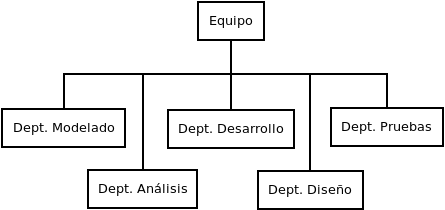
\includegraphics[scale=0.70]{imagenes/diagramaEstructura.png}
	\caption{\label{fig:diagramaEstructura}Diagrama estructura del formulario OM2}
\end{figure}




 






	
	%%%%%%%%%%%%%%%%%%%%%%%%%%%%%%%%%%%%%%%%%%%%%%%%%%%%%%%%%%%%%%%%%%%%%%%%
% Plantilla TFG/TFM
% Universidad de A Coruña. Facultad de Informática
% Realizado por: Welton Vieira dos Santos
% Modificado: Welton Vieira dos Santos
% Contacto: welton.dossantos@udc.es
%%%%%%%%%%%%%%%%%%%%%%%%%%%%%%%%%%%%%%%%%%%%%%%%%%%%%%%%%%%%%%%%%%%%%%%%


\chapter{Desarrollo técnico}
\section{Videojuego en 2D}
\subsection{Descripción}

 


 






	
	%%%%%%%%%%%%%%%%%%%%%%%%%%%%%%%%%%%%%%%%%%%%%%%%%%%%%%%%%%%%%%%%%%%%%%%%%
% Plantilla TFG/TFM
% Universidad de A Coruña. Facultad de Informática
% Realizado por: Welton Vieira dos Santos
% Modificado: Welton Vieira dos Santos
% Contacto: welton.dossantos@udc.es
%%%%%%%%%%%%%%%%%%%%%%%%%%%%%%%%%%%%%%%%%%%%%%%%%%%%%%%%%%%%%%%%%%%%%%%%


\chapter{Modelo de conocimiento}
\newpage
\section{Fase de identificación}
\subsection{Tareas del formulario OM-3}
La tarea elegida para este modelo conceptual ha sido la tarea 5 del OM-3 (Tabla \ref{tab:IdentificacionOM3}), que corresponde con la \textbf{Gestión de las Operativas Abiertas}.

\begin{table}[H]
  \centering
  \resizebox{18,0cm}{!}{
    \begin{tabular}{|c|c|c|c|c|c|c|}
      \hline
      \multicolumn{3}{|c}{\textbf{Modelo de Organización}} & \multicolumn{4}{|c|}{\textbf{Formulario OM-3: Descomposición de los Procesos}}\\
      \hline \hline
      \textsc{N\textordmasculine} & \textsc{Tarea} & \textsc{Realiza\-da por} & \textsc{¿Dónde?} & \textsc{Recursos de Conocimiento} & \textsc {¿In\-ten\-si\-va en Conocimiento?} & \textsc{Im\-por\-tan\-cia} \\
      \hline
            
      5 & \multicolumn{1}{|p{6.0cm}|}{\centering Gestionar las operativas abiertas} & \multicolumn{1}{|p{6.0cm}|}{\centering Inversor (usuario)} &  \multicolumn{1}{|p{5.0cm}|}{\centering En PC del inversor (usuario)} & \multicolumn{1}{|p{6.0cm}|}{\centering Experiencia en gestionar las operativas de compra y venta de activos al mercado de divisas. Teorías de gestión de capital de inversión} & Sí (elevado) & Máxima \\
      \hline
    \end{tabular}
  }
	\caption{\label{tab:IdentificacionOM3}Tarea elegida para el modelo de conocimiento}
\end{table}

\subsection{Glosario de términos}
\begin{itemize}
	\item \textbf{Activo:} Entidad en la que se prentende especular, que en caso de Forex, hay una variabilidad de 26 pares de divisas, por ejemplo, EURUSD - Euro contra el Dolar.
	\item \textbf{Tendencia Alcista:} es una tendencia del mercado bulsátil donde los precios de los activos financieros llegan a nuevos máximos comparando en un mismo período de análisis. Ejemplo en la imagen de la izquierda de la Figura \ref{fig:EjemploTentendias}.
	\item \textbf{Tendencia Bajista:} es una tendencia del mercado bulsátil donde los precios de los activos financieros llegan a nuevos mínimos comparando en un mismo período de análisis. Ejemplo en la imagen de la derecha de la Figura \ref{fig:EjemploTentendias}.
	\item \textbf{Soporte:} Un soporte es un nivel de precio por debajo del actual, se espera que la fuerza de compra supere a la de venta, por lo que un impulso bajista se verá frenado y por lo tanto el precio repuntará. Normalmente, un soporte corresponde a un mínimo alcanzado anteriormente. Ejemplos en la Figura \ref{fig:SoportesResistencias} se muestra como lineas horizontales de color azul (S1,S2,\dots,SN)
	\item \textbf{Resistencia:} Una resistencia es el concepto opuesto a un soporte. Es un precio por encima del actual, la fuerza de venta superará a la de compra, poniendo fin al impulso alcista, y por lo tanto el precio retrocederá. Ejemplos en la Figura \ref{fig:SoportesResistencias} se muestra como lineas horizontales de color azul (S1,S2,\dots,SN).
	\item \textbf{Stop Loss:} Son límites máximos de pérdida puesto por parte del inversor para frenar una situación de pérdida.
\end{itemize}

\begin{figure}[H]
	\centering
	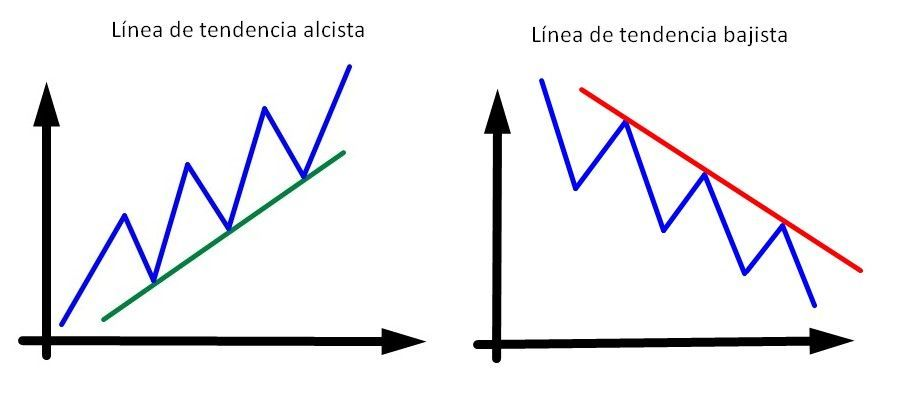
\includegraphics[scale=0.45]{imagenes/EjemploTentendias.png}
	\caption{\label{fig:EjemploTentendias}Ejemplo de tendencias de mercado}
\end{figure}

\begin{figure}[H]
	\centering
	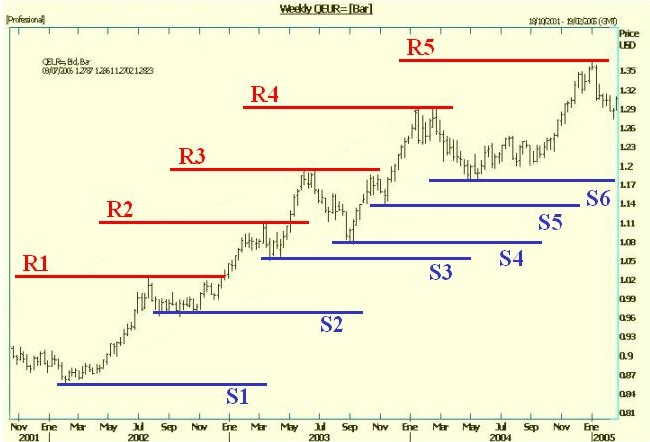
\includegraphics[scale=0.45]{imagenes/SoportesResistencias.png}
	\caption{\label{fig:SoportesResistencias}Soportes y resistencias del Euro/Dólar de 2001 a 2005}
\end{figure}

\subsection{Descripción de escenarios}
\begin{enumerate}
	\item  \textbf{Escenario de reducción de riesgo de una orden de compra (Buy):} En la situación que se muestra en la Figura \ref{fig:Situacion1}, donde el inversor había ejecutado una orden de compra en el precio \textbf{1.18767} y ha estipulado su gestión de riesgo para el precio \textbf{1.18664} y como se observa en el gráfico de la figura comentada anteriormente, el precio esta a favor del inversor y en esa ocasión el inversor tiene que reducir el riesgo inicial de la inversión al precio \textbf{1.19516} como se muestra en la Figura \ref{fig:Situacion12}.	
	\item  \textbf{Escenario de gestión de ganancia en una orden de compra (Buy)}: En la situación que se muestra en la Figura \ref{fig:Situacion2}, donde el inversor había ejecutado una orden de compra en el precio \textbf{1.18767} y ha estipulado su gestión de riesgo para el precio \textbf{1.18664} y como se observa en el gráfico de la figura comentada anteriormente, el precio esta a favor del inversor y el mismo decide cerrar esa operativa a precio del mercado, que en ese caso es de \textbf{1.19665}.	
\end{enumerate}
\begin{figure}[H]
    \centering
    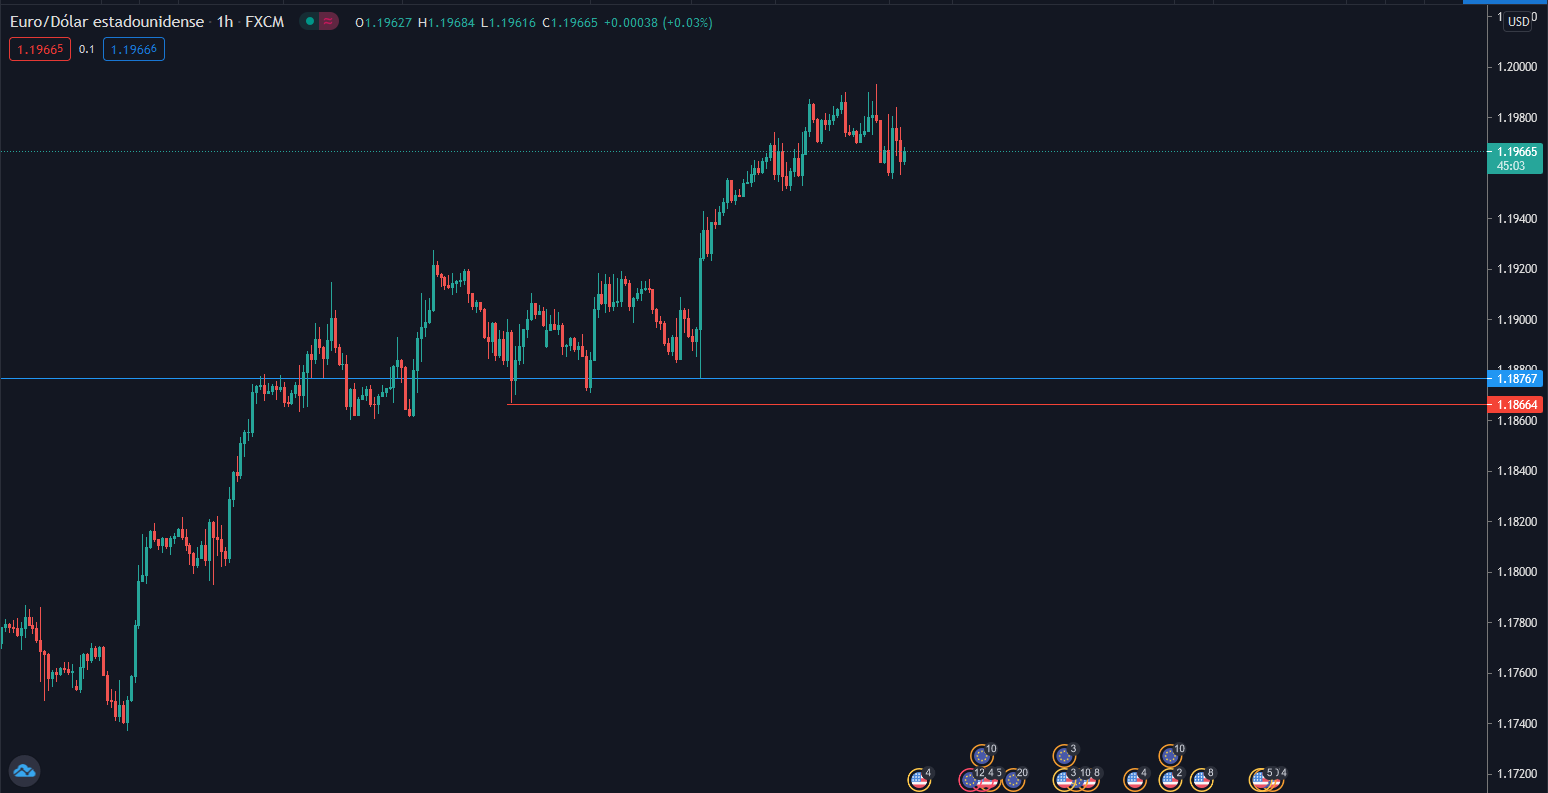
\includegraphics[scale=0.30]{imagenes/Situacion1.png}
    \caption{\label{fig:Situacion1}Ejemplo de una situación donde el inversor tiene que ajustar el riesgo de la operativa y seguir dentro del mercado}
  \end{figure}
\begin{figure}[H]
  \centering
  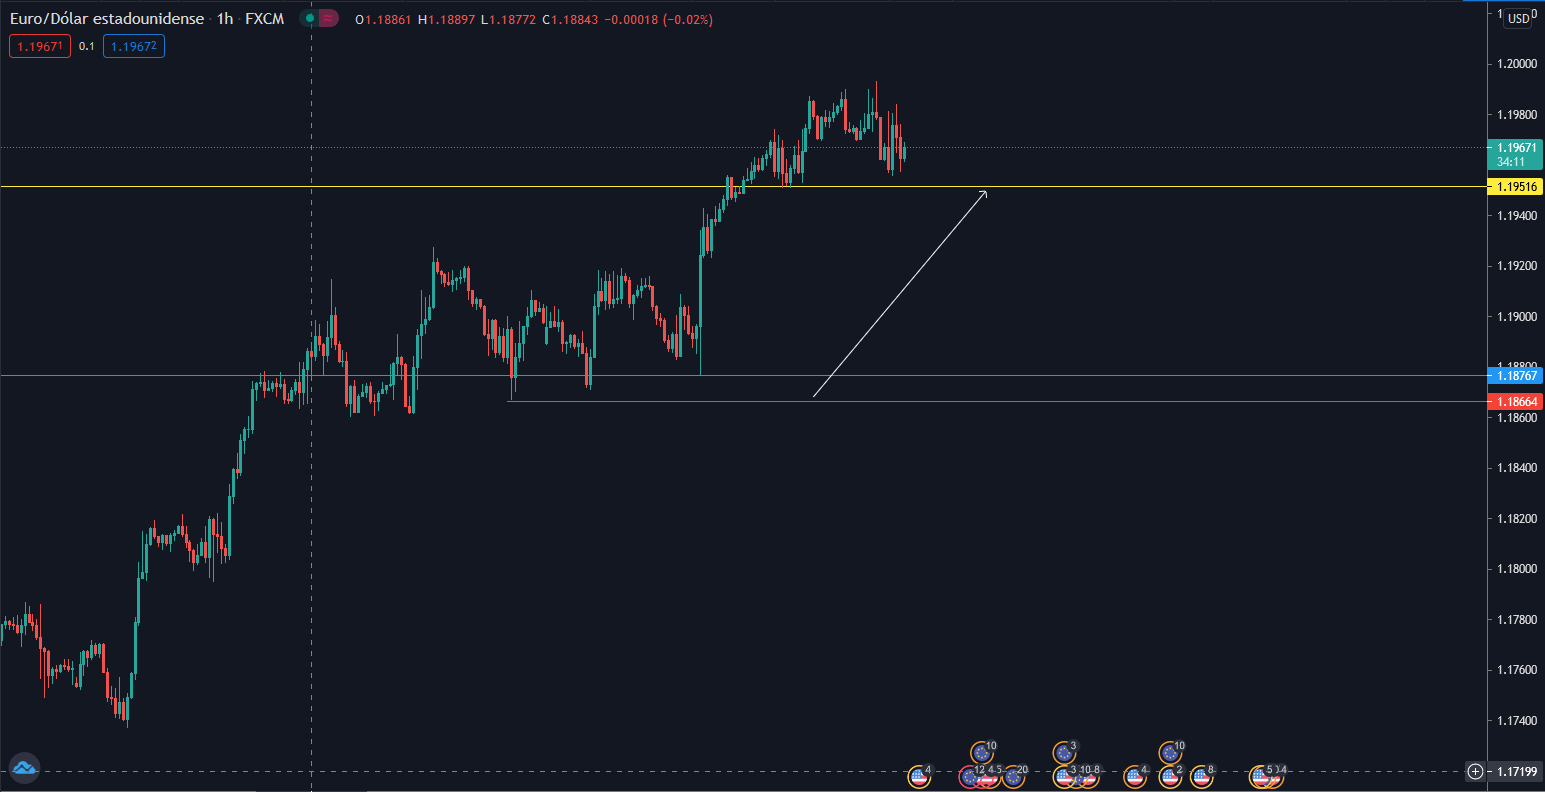
\includegraphics[scale=0.30]{imagenes/Situacion12.png}
  \caption{\label{fig:Situacion12}Ejemplo donde el inversor modifica el nivel de riesgo inicial y mantiene la orden de compra en el mercado}
\end{figure}
\begin{figure}[H]
  \centering
  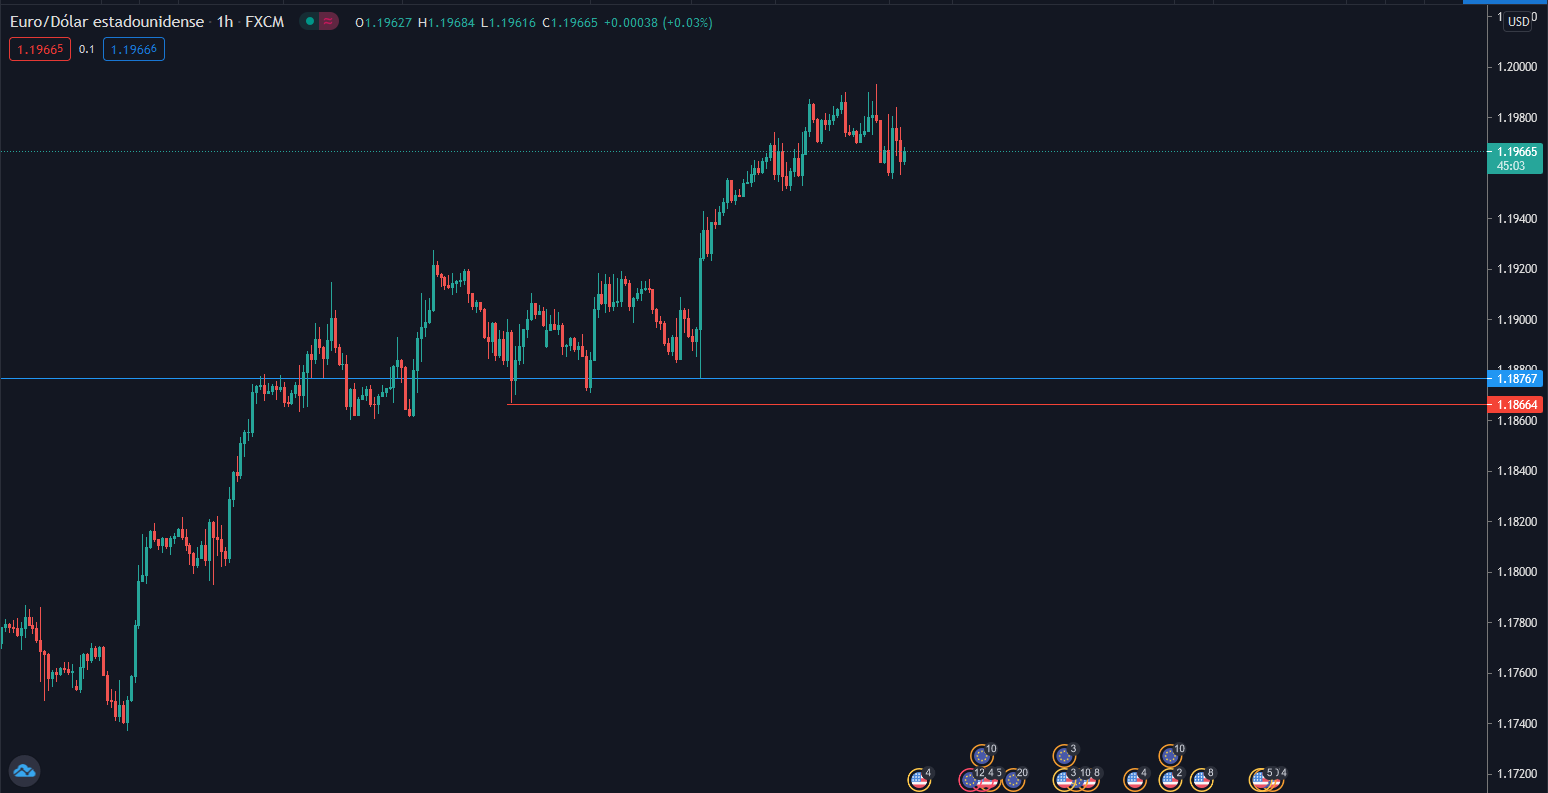
\includegraphics[scale=0.30]{imagenes/Situacion1.png}
  \caption{\label{fig:Situacion2}Ejemplo donde el inversor decide cerrar la orden de compra a precio de mercado}
\end{figure}

\section{Fase de especificación}
\subsection{Justificación de la selección de la metodología}
Para este proyecto hemos decidido utilizar la metodología ``middle-out'' con la selección de la plantilla de diagnóstico, ya que esa plantilla nos permite tomar varias decisiones un proyecto anterior con la misma metodología ``middle-out'', puesto que, además ser muy utilizada en nuestro caso sigue adaptandose perfectamente. 

\subsection{Plantilla anotada}

La plantilla que mas se adapta a nuestro problema es la de diagnóstico, como se muestra en la Figura \ref{fig:PlantillaEjemplo}. Con una pequeña modificación que se muestras en la Figuras \ref{fig:PlantillaDiagnosticoModificada}.

\begin{figure}[H]
  \centering
  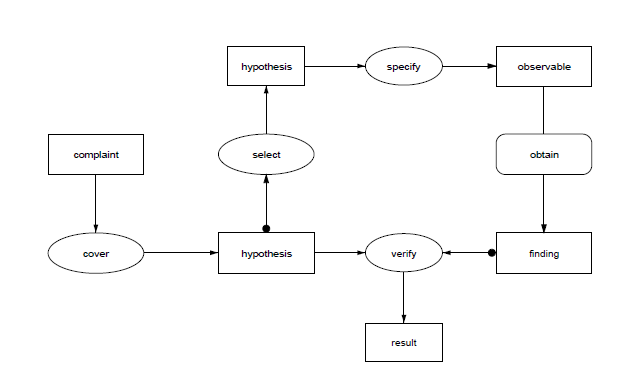
\includegraphics[scale=0.90]{imagenes/PlantillaEjemplo.png}
  \caption{\label{fig:PlantillaEjemplo}Ejemplo de la plantilla elegida}
\end{figure}

\begin{figure}[H]
  \centering
  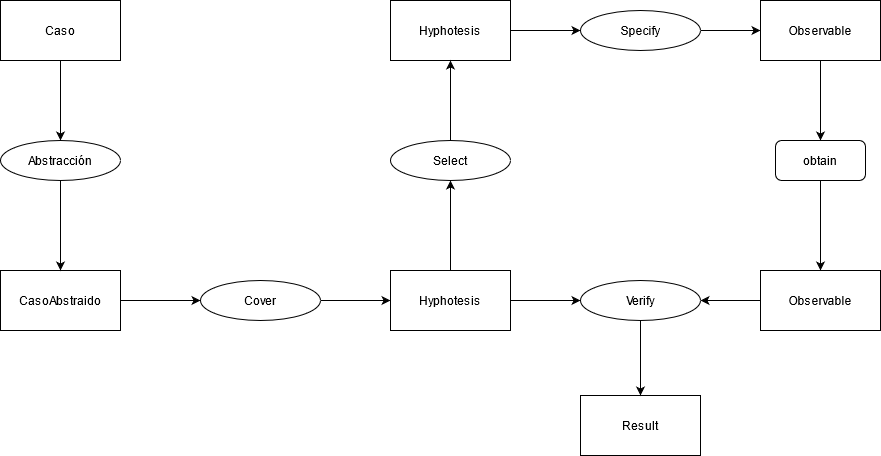
\includegraphics[scale=2.10]{imagenes/PlantillaDiagnosticoModificada.png}
  \caption{\label{fig:PlantillaDiagnosticoModificada}Ejemplo de la plantilla diagnóstico modificada}
\end{figure}

\subsubsection{Anotaciones}
Comentarios y ejemplos concretos para los roles presentes en la plantilla seleccionada.
\begin{itemize}
  \item \textbf{Caso:} Datos de una operativa: e.g. En la situación que se muestra en la Figura \ref{fig:Situacion1}, donde el inversor había ejecutado una orden de compra en el precio \textbf{1.18767} y ha estipulado su gestión de riesgo para el precio \textbf{1.18664} y como se observa en el gráfico de la figura comentada anteriormente, el precio esta a favor del inversor y en esa ocasión el inversor tiene que reducir el riesgo inicial de la inversión una vez superada la resistencia.
  \item \textbf{Caso abstraído:} Datos de una operativa abstaídos. e.g. El precio del activo ha superado la resistencia, es decir, MercadoForex.Activo.valor > resistencia. Se abstrae en MercadoForex.Activo.valor > MercadoForex.resistencia.Fuerte
  \item \textbf{Hypothesis\footnote{Hypothesis (Diferential)}:} Posibles acciones a llevar a cabo e.g. Cerrar la operativa o reducir el riesgo.
  \item \textbf{Hypothesis\footnote{Hypothesis (Hypothesis)}:} Acción concreta a evaluar. e.g. reducir el riesgo.
  \item \textbf{Observable:} Estado del mercado de forex para la operativa actual. e.g. Mercado forex para EURUSD.
  \item \textbf{Finding:} Estado del mercado con respecto a nuestra operativa: e.g. Si estamos comprando que la tendencia sea alcista o si estamos vendiendo bajista.
  \item \textbf{Result:} Se confirma o deniega la hipotesis seleccionada. e.g. \{Ajustar riesgo = True, Cerrar la operativa = False\} 
\end{itemize}

\subsection{Esquema inicial del dominio}

\begin{figure}[H]
  \centering
  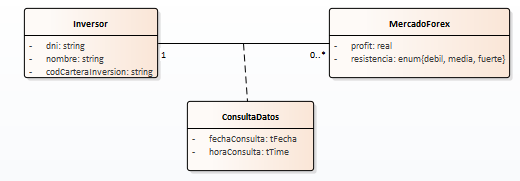
\includegraphics[scale=0.90]{imagenes/DominioInicial.png}
  \caption{\label{fig:DominioInicial}Dominio inicial}
\end{figure}

\subsection{Estructura inferencial}
\subsubsection{Plantilla}
\subsubsection{Mapeado}
Relacción entre los roles de las inferencias de la plantilla con los conceptos de nuestro problema.
\begin{itemize}
  \item Abstraído:
  \begin{figure}[H]
    \centering
    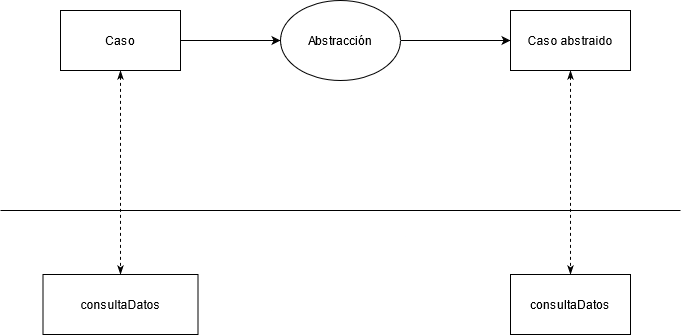
\includegraphics[scale=0.50]{imagenes/abstraccion.png}
    \caption{\label{fig:Cover}Ejemplo del mapeo de Abstraccion}
  \end{figure}
  \item Cover:  
  \begin{figure}[H]
    \centering
    \includegraphics[scale=0.50]{imagenes/cover.png}
    \caption{\label{fig:Cover}Ejemplo del mapeo de Cover}
  \end{figure}
  \item Select: 
  \begin{figure}[H]
    \centering
    \includegraphics[scale=0.50]{imagenes/select.png}
    \caption{\label{fig:Select}Ejemplo del mapeo de Select}
  \end{figure}
  \item Specify: 
  \begin{figure}[H]
    \centering
    \includegraphics[scale=0.50]{imagenes/specify.png}
    \caption{\label{fig:Specify}Ejemplo del mapeo de Specify}
  \end{figure}
  \item Obtain:  
  \begin{figure}[H]
    \centering
    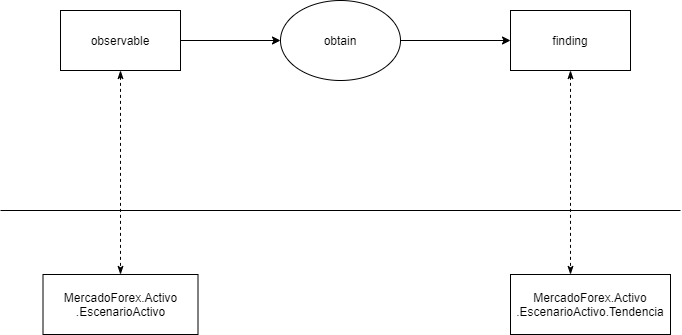
\includegraphics[scale=0.50]{imagenes/Obtain.png}
    \caption{\label{fig:Obtain}Ejemplo del mapeo de Obtain}
  \end{figure}
  \item Verify:  
  \begin{figure}[H]
    \centering
    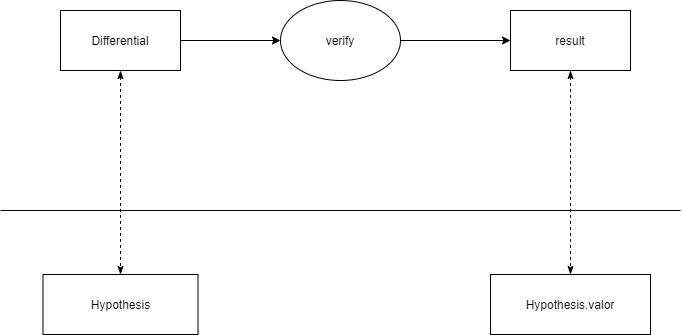
\includegraphics[scale=0.50]{imagenes/verify1.png}
    \caption{\label{fig:Verify}Ejemplo del mapeo de Verify del rol Diferential}
  \end{figure}
  \begin{figure}[H]
    \centering
    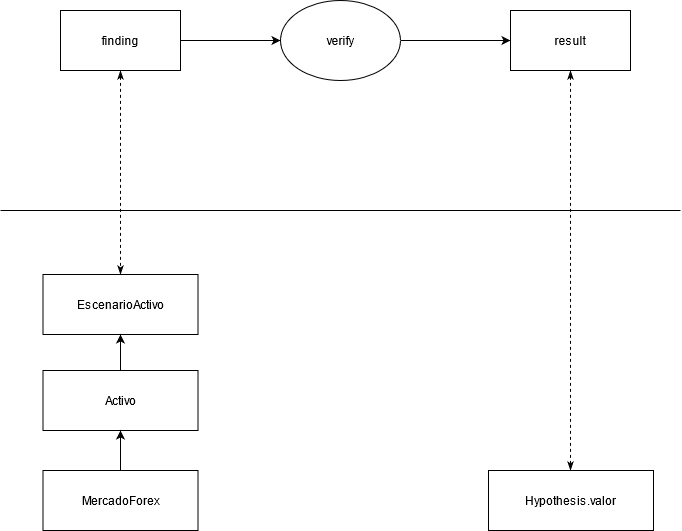
\includegraphics[scale=0.50]{imagenes/verify2.png}
    \caption{\label{fig:verify2}Ejemplo del mapeo de Verify del rol finding}
  \end{figure}
\end{itemize}

\section{Especificación y método de la tarea}	
	%\input{capitulos/Tema_5}	
	%\input{capitulos/Tema_6}	
	
	%\input{capitulos/5_conclusiones}
	%\includepdf[pages={57-97}]{archivos/plantilla-tfg-fium.pdf}
	%%%%%%%%%%%%%%%%%%%%%%%%%%%%%%%%%%%%%%%%%%%%%%%%%%%%%%%%%%%%%%%%%%%%%%%%%
% Plantilla para escribir libros
% Universidad de A Coruña. Facultad de Informática
% Realizado por: Welton Vieira dos Santos
% Modificado: Welton Vieira dos Santos
% Contacto: welton.dosssantos@udc.es
%%%%%%%%%%%%%%%%%%%%%%%%%%%%%%%%%%%%%%%%%%%%%%%%%%%%%%%%%%%%%%%%%%%%%%%%

\chapter{Introducción (Con ejemplos de contenido)}

Antes de comenzar la lectura de este documento debo agradecer el trabajo realizado por Pedro Pernías Peco en su plantilla de ``tfg'' que se puede ver en \url{https://github.com/lcg51/tfg}. Gracias a esa plantilla me he lanzado a crear mi versión. Algunos contenidos aquí mostrados han sido extraídos de la plantilla de Pedro. 
\\
\par Esta plantilla se ha diseñado de 0 y por ello no utiliza la misma estructura que la plantilla de Pedro. Pero la estructura de contenido para un TFG/TFM es la misma y a continuación se muestran las diferentes partes que debe tener un TFG/TFM redactado por Pedro.
\section{¡Importante!, leer primero}

Este texto está escrito pensando en orientar a los alumnos que usarán \LaTeX~para escribir su \gls{tfg} y \gls{tfm}. 
\\
\par Contiene información útil para aquellos que no tengan experiencia previa en \LaTeX~así como algunos datos acerca de cómo escribir mejor su \gls{tfg}.
A continuación, se ofrece una copia de la información que hay en el libro de estilo para la realización de los \gls{tfg} de la EPS de la Universidad de Alicante.

En los capítulos siguientes encontrarás ejemplos de muchas de las cosas que se pueden realizar con \LaTeX. Con un poco de paciencia, estudia cómo se hacen estas cosas y luego aplícalas en tus documentos.


\section{Estructura de un \glsentryshort{tfg}}

En caso de que el \gls{tfg}/\gls{tfm} tenga como finalidad la elaboración de un proyecto o un 
informe científico o técnico, deberá ajustarse a lo dispuesto en las normas UNE 
157001:2002 y UNE 50135:1996 respectivamente.

Si el \gls{tfg}/\gls{tfm} tiene por finalidad la elaboración de un trabajo monográfico, el 
documento presentado deberá constar de las siguientes partes, teniendo como base la 
norma UNE 50136:1997.

\begin{description}
\item[Preámbulo:] se describirán brevemente la motivación que ha originado la realización del \gls{tfg}/\gls{tfm}, así como una breve descripción de los objetivos generales que se quieren alcanzar con el trabajo presentado.
\item[Agradecimientos:] se podrán añadir las hojas necesarias para realizar los agradecimientos, a veces obligatorios, a las entidades y organismos colaboradores.
\item[Dedicatoria:] se podrá añadir una única hoja con dedicatorias, su alineación será derecha.
\item[Citas:] (frases célebres) se podrá añadir una única hoja con citas, su alineación será derecha.
\item[Índices:] cada índice debe comenzar en una nueva página, se incluirán los índices que se estimen necesarios (conforme UNE 50111:1989), en este orden:
\begin{description}
\item[Índice de contenidos:] (obligatorio siempre) se incluirá un índice de las secciones de las que se componga el documento, la numeración de las 
divisiones y subdivisiones utilizarán cifras arábigas (según UNE 50132:1994) y harán mención a la página del documento donde se ubiquen.
\item[Índice de figuras:] si el documento incluye figuras se podrá incluir también un índice con su relación, indicando la página donde se ubiquen.
\item[Índice de tablas:] en caso de existir en el texto, ídem que el anterior.
\item[Índice de abreviaturas, siglas, símbolos, etc.:] en caso de ser necesarios se podrán incluir cada uno de ellos.
\end{description}
\item[Cuerpo del documento:] en el contenido del documento se da flexibilidad para su organización y se puede estructurar en las secciones que se considere. En todo caso obligatoriamente se deberá, al menos, incluir los siguientes contenidos:
\begin{description}
\item[Introducción:] donde se hará énfasis a la importancia de la temática, su vigencia y actualidad; se planteará el problema a investigar, así como el propósito o finalidad de la investigación.
\item[Marco teórico o Estado del arte:] se hará mención a los elementos conceptuales que sirven de base para la investigación, estudios previos relacionados con el problema planteado, etc.
\item[Objetivos:] se establecerán el objetivo general y los específicos.
\item[Metodología:] se indicarán el tipo o tipos de investigación, las técnicas y los procedimientos que serán utilizados para llevarla a cabo; se identificarán la población y el tamaño de la muestra así como las técnicas e instrumentos de recolección de datos.
\item[Resultados:] incluirá los resultados de la investigación o trabajo, así como el análisis y la discusión de los mismos.
\end{description}
\item[Conclusiones:] obligatoriamente se incluirá una sección de conclusiones donde se realizará un resumen de los objetivos conseguidos así como de los resultados obtenidos si proceden.
\item[Bibliografía y referencias:] se incluirá también la relación de obras y materiales consultados y empleados en la elaboración de la memoria del \gls{tfg}/\gls{tfm}. La bibliografía y las referencias serán indexadas en orden alfabético (sistema nombre y fecha) o se numerará correlativamente según aparezca (sistema numérico). Se empleará la familia 1 como tipo de letra. Podrá utilizarse cualquier sistema bibliográfico normalizado predominante en la rama de conocimiento, estableciéndose como prioritarios el sistema ISO 690, sistema \gls{apa}  o Harvard (no necesariamente en ese orden de preferencia). En esta plantilla Latex se propone usar el estilo \gls{apa} indicándolo en la línea correspondiente como 
\begin{verbatim}
\bibliographystyle{unsrtnat}
\end{verbatim}


\item[Anexos:] se podrán incluir los anexos que se consideren oportunos.

\end{description}

\section{Apartados dentro de los capítulos}
En \LaTeX~existen diferentes niveles de títulos para realizar secciones, subsecciones, etc. En esta web puedes ver más información al respecto \url{https://en.wikibooks.org/wiki/LaTeX/Document_Structure}

Para ello se utilizan los siguientes comandos;

\begin{lstlisting}[style=Latex-color]
	\section{Esto es una sección}
	Y este el contenido de la sección.
	\subsection{Esto es una subsección}
	Y este el contenido de la subsección.
	\subsubsection{Esto es una subsubsección}
	Y este el contenido de la subsubsección.
	\paragraph{Esto es un paragraph}
 	Y este el contenido del paragraph. Que siempre se inicia en la misma línea que el título del mismo.
\end{lstlisting}
 Y se genera lo siguiente:
 \section{Esto es una sección}
	Y este el contenido de la sección.
	\subsection{Esto es una subsección}
	Y este el contenido de la subsección.
	\subsubsection{Esto es una subsubsección}
	Y este el contenido de la subsubsección.
	\paragraph{Esto es un paragraph}
 	Y este el contenido del paragraph. Que siempre se inicia en la misma línea que el título del mismo.

\section{Citar bibliografía}
Para citar la bibliografía tal como se define en el sistema APA (en esta web se indica como debe aparecer en el texto la cita: \url{http://guides.libraries.psu.edu/apaquickguide/intext}) se debe realizar con alguno de los comandos mostrados a continuación:

\begin{lstlisting}[style=Latex-color]
Esto es una cita estándar: \citet{Shaw1996}, que también puedes mostrar con paréntesis así: \citep{Shaw1996}. También se puede realizar una cita indicando a qué parte te refieres \citep[ver][Cap. 2]{Shaw1996} o \cite[Cap. 2]{Shaw1996} o \citep[ver][]{Shaw1996}. 

También puedes mostrar todos los autores cuando hay más de 2 autores añadiendo un asterisco después del comando como: \citet*{Akyildiz2005}, sin el asterisco quedaría así: \citet{Akyildiz2005}.

O puedes citar dos o más fuentes al mismo tiempo: \citep{Barkan1995,Leighton2012}

\cite{UNE50136:97}

\end{lstlisting}
Y \LaTeX~genera lo siguiente:
\\
\par Esto es una cita estándar: \citet{Shaw1996}, que también puedes mostrar con paréntesis así: \citep{Shaw1996}. También se puede realizar una cita indicando a qué parte te refieres \citep[ver][Cap. 2]{Shaw1996} o \citep[Cap. 2]{Shaw1996} o \citep[ver][]{Shaw1996}. 
\\
\par También puedes mostrar todos los autores cuando hay más de 2 autores añadiendo un asterisco después del comando como: \citet*{Akyildiz2005}, sin el asterisco quedaría así: \citet{Akyildiz2005}.
\\
\par O puedes citar dos o más fuentes al mismo tiempo: \citep{Barkan1995,Leighton2012}


\section{Notas a pie de página}

Para introducir notas a pie de página se debe escribir lo siguiente:

\begin{lstlisting}[style=Latex-color]
	La plantilla necesita el motor XeLaTeX \footnote{Para más información sobre XeLaTeX visita \url{https://es.sharelatex.com/learn/XeLaTeX}} (el más recomendable actualmente), por lo que si el programa que utilizas compila la plantilla con el motor pdfLaTeX \footnote{También puedes buscar más información en internet} (el más habitual pero menos potente) debes cambiarlo por XeLaTeX en las opciones del programa. Si no sabes como hacerlo busca en el manual del programa o en google.
\end{lstlisting}

\LaTeX~genera lo siguiente (observa las notas a pie de página):
\\
\par La plantilla necesita el motor XeLaTeX\footnote{Para más información sobre XeLaTeX visita \url{https://es.sharelatex.com/learn/XeLaTeX}} (el más recomendable actualmente), por lo que si el programa que utilizas compila la plantilla con el motor pdfLaTeX\footnote{También puedes buscar más información en internet} (el más habitual pero menos potente) debes cambiarlo por XeLaTeX en las opciones del programa. Si no sabes como hacerlo busca en el manual del programa o en google.
\section{Estilos de texto}

A continuación se muestran ejemplos de distintos estilos de texto:

\begin{itemize}
	\item \textbackslash textit\{Cursiva\} $\rightarrow$ \textit{Cursiva}
	\item \textbackslash emph\{Cursiva 2\} $\rightarrow$ \emph{Cursiva 2}
	\item \textbackslash textbf\{Negrita\} $\rightarrow$ \textbf{Negrita}
	\item \textbackslash texttt\{Monoespacio\} $\rightarrow$ \texttt{Monoespacio}
	\item \textbackslash textsc\{Mayúsculas capitales\} $\rightarrow$ \textsc{Mayúsculas capitales}
	\item \textbackslash uppercase\{Todo mayúsculas\} $\rightarrow$ \uppercase{Todo mayúsculas} 
\end{itemize}

 \section{Acrónimos}
 Ahora vamos a ver cómo se ponen los acrónimos.
 
 La norma dice que la primera vez que aparece un acrónimo debe ponerse su fórmula completa, es decir lo que significa, al lado del acrónimo. Después de ello, podemos usar sólo el acrónimo salvo cuando consideremos que debemos volver a usar la fórmula completa por alguna razón de legibilidad.
 
 ¿Cómo llevar la cuenta de cuándo es la primera vez que ponemos el acrónimo? si hacemos cambios en el doc es fácil que perdamos esa información así que lo mejor es que sea el propio \LaTeX~el que lleve esa cuenta. Para ello tenemos que hacer dos cosas:
 \begin{description}
 \item[Primero:] creamos la entrada del acrónimo en el fichero acronimos.tex. Revisa los comentarios de su cabecera para saber cómo crear esa entrada. Básicamente lo que hacemos allí es poner la ``fórmula corta'' y la ``fórmula larga'' del acrónimo es decir, el propio acrónimo y su significado
 \item[Segundo:] escribimos en el texto el acrónimo SIEMPRE diciendo que es un acrónimo y el tipo de fórmula que queremos usar. Por ejemplo, si siempre que queremos hacer referencia al IEEE escribimos \begin{lstlisting}[style=Latex-color]
 \gls{ieee}
 \end{lstlisting}  se consigue que la primera vez que aparezca el acrónimo ponga las fórmulas larga y corta y en las siguientes ocasiones sólo aparecerá la corta.
 \end{description}
 
 Aquí va un ejemplo:
 
 Si escribimos:
 
\begin{lstlisting}[style=Latex-color]
 El \gls{ieee} es una institución muy importante en el mundo de la
 ingeniería.  El \gls{ieee} lleva marcando normas y protocolos desde
 hace mucho tiempo.  Pero el \gls{ieee} no está solo en esta tarea. 
 Además del \gls{ieee} hay muchas otras instituciones para ello.  \end{lstlisting}
 
 Obtendremos: 
 
El \gls{ieee} es una institución muy importante en el mundo de la
 ingeniería.  El \gls{ieee} lleva marcando normas y protocolos desde
 hace mucho tiempo.  Pero el \gls{ieee} no está solo en esta tarea. 
 Además del \gls{ieee} hay muchas otras instituciones para ello.
 
 \section{Tareas por hacer}
 
 En esta plantilla se ha incluido un paquete para incluir notas/comentarios en el texto para recordar partes que hay que revisar o terminar de desarrollar. El uso es sencillo, el manual para conocer todos los comandos se encuentra en \url{http://osl.ugr.es/CTAN/macros/latex/contrib/todonotes/todonotes.pdf}, a continuación se muestran algunos ejemplos:
 \\
\par Para incluir un comentario sobre el texto:

\begin{lstlisting}[style=Latex-color]
	Recomiendo utilizar programas LaTeX que permitan trabajar con sistema de archivos para poder editar el conjunto de capítulos en la misma ventana. Este tipo de función lo tienen programas como TexStudio, es multiplataforma. \todo{Incluir más ejemplos de programas}
\end{lstlisting}

\LaTeX~genera lo siguiente:
\\
\par Recomiendo utilizar programas LaTeX que permitan trabajar con sistema de archivos para poder editar el conjunto de capítulos en la misma ventana. Este tipo de función lo tienen programas como TexStudio, es multiplataforma. \todo{Incluir más ejemplos de programas}
\vspace{1em}
\noindent\hrule
\vspace{1em}
\par Para incluir un comentario sobre el texto pero dentro del texto:

\begin{lstlisting}[style=Latex-color]
	Recomiendo utilizar programas LaTeX que permitan trabajar con sistema de archivos para poder editar el conjunto de capítulos en la misma ventana. Este tipo de función lo tienen programas como TexStudio, es multiplataforma. \todo[inline]{Incluir más ejemplos de programas}
\end{lstlisting}

\LaTeX~genera lo siguiente:
\\
\par Recomiendo utilizar programas LaTeX que permitan trabajar con sistema de archivos para poder editar el conjunto de capítulos en la misma ventana. Este tipo de función lo tienen programas como TexStudio, es multiplataforma. \todo[inline]{Incluir más ejemplos de programas}
\vspace{1em}
\noindent\hrule
\vspace{1em}
\par También se puede dejar indicado donde falta una imagen o figura, para incluirla más adelante del siguiente modo:

\begin{lstlisting}[style=Latex-color]
\missingfigure{Añadir gráfica de rendimiento}	
\end{lstlisting}

\LaTeX~genera lo siguiente:
\\
\missingfigure{Añadir gráfica de rendimiento}	



		% Plantilla: Se muestran contenidos
	%%%%%%%%%%%%%%%%%%%%%%%%%%%%%%%%%%%%%%%%%%%%%%%%%%%%%%%%%%%%%%%%%%%%%%%%%
% Plantilla para escribir libros
% Universidad de A Coruña. Facultad de Informática
% Realizado por: Welton Vieira dos Santos
% Modificado: Welton Vieira dos Santos
% Contacto: welton.dosssantos@udc.es
%%%%%%%%%%%%%%%%%%%%%%%%%%%%%%%%%%%%%%%%%%%%%%%%%%%%%%%%%%%%%%%%%%%%%%%%

\chapter{Marco Teórico (Con ejemplos de listas)}
\label{marcoteorico}

\section{Listas}
Hacer una lista es simple en \LaTeX. Para ello has de crear un entorno (así se llama) itemize con
\begin{lstlisting}[style=Latex-color]
\begin{itemize}
...
\end{itemize}
\end{lstlisting}
Y dentro de esa estructura, añadir cada elemento de la lista precedido de 
\begin{lstlisting}[style=Latex-color]
\item primer ítem de lista
\item segundo ítem de lista
...
\item ultimo ítem de lista
\end{lstlisting}

Es importante que revises este texto tal como aparece en la plantilla y relaciones el aspecto que tiene el PDF final con cómo está escrito el documento \LaTeX.
\vspace{1em}
\noindent\hrule
\vspace{1em}

Aquí va una lista con subtérminos:
\begin{lstlisting}[style=Latex-color]
	\begin{itemize}
    \item Ingeniería Informática.
    \item Ingeniería Sonido e Imagen en Telecomunicación.
    \item Ingeniería Multimedia.
         \subitem Mención: Creación y ocio digital.
         \subitem Mención: Gestión de Contenidos.
	\end{itemize}
\end{lstlisting}

El resultado es el siguiente:
\begin{itemize}
    \item Ingeniería Informática.
    \item Ingeniería Sonido e Imagen en Telecomunicación.
    \item Ingeniería Multimedia.
         \subitem Mención: Creación y ocio digital.
         \subitem Mención: Gestión de Contenidos.
\end{itemize}
\vspace{1em}
\noindent\hrule
\vspace{1em}
Aquí va una lista con subtérminos pero numerada:
\begin{lstlisting}[style=Latex-color]
\begin{enumerate}
    \item Ingeniería Informática.
    \item Ingeniería Sonido e Imagen en Telecomunicación.
    \item Ingeniería Multimedia.
    \begin{enumerate}
         \item Mención: Creación y ocio digital.
         \item Mención: Gestión de Contenidos.
   	\end{enumerate}
\end{enumerate}
\end{lstlisting}

El resultado es el siguiente:
\begin{enumerate}
    \item Ingeniería Informática.
    \item Ingeniería Sonido e Imagen en Telecomunicación.
    \item Ingeniería Multimedia.
    \begin{enumerate}
         \item Mención: Creación y ocio digital.
         \item Mención: Gestión de Contenidos.
   	\end{enumerate}
\end{enumerate}

\section{Listas de definición}
 
 Puedes realizar una lista de conceptos con su definición del siguiente modo:
 
\begin{lstlisting}[style=Latex-color]
\begin{description} % Inicio de la lista
 	\item[MAPP XT:] Programa desarrollado por \textit{Meyer Sound} para el diseño y ajuste de sistemas formados por altavoces de su marca.
  	\begin{description} % Realiza una lista dentro de la lista
  		\item[Ventajas:]~ 
  		El programa permite realizar múltiples ajustes tal como se podría realizar en la realidad con un procesador real.
  	
  		Permite analizar la fase recibida en cualquier punto y compararla con otras mediciones.
  	
  		Dispone de varios tipos de filtros, inversiones de fase, etc.
  		\item[Inconvenientes:]~ 
  		No existe una lista global de los altavoces ubicados en el plano, por lo tanto solo se pueden editar seleccionándolos sobre el plano.
  	
  		Sólo permite diseñar en 2 dimensiones, principalmente sobre la vista lateral ya que los array de altavoces no permite voltearlos.
  	\end{description}
\end{description}
\end{lstlisting}

 Y \LaTeX~genera lo siguiente:
 
\begin{description} % Inicio de la lista
 	\item[MAPP XT:] Programa desarrollado por \textit{Meyer Sound} para el diseño y ajuste de sistemas formados por altavoces de su marca.
  	\begin{description} % Realiza una lista dentro de la lista
  		\item[Ventajas:]~ 
  		El programa permite realizar múltiples ajustes tal como se podría realizar en la realidad con un procesador real.
  	
  		Permite analizar la fase recibida en cualquier punto y compararla con otras mediciones.
  	
  		Dispone de varios tipos de filtros, inversiones de fase, etc.
  		\item[Inconvenientes:]~ 
  		No existe una lista global de los altavoces ubicados en el plano, por lo tanto solo se pueden editar seleccionándolos sobre el plano.
  	
  		Sólo permite diseñar en 2 dimensiones, principalmente sobre la vista lateral ya que los array de altavoces no permite voltearlos.
  	\end{description}
\end{description}		% Plantilla: Se muestran listas
	%%%%%%%%%%%%%%%%%%%%%%%%%%%%%%%%%%%%%%%%%%%%%%%%%%%%%%%%%%%%%%%%%%%%%%%%%
% Plantilla para escribir libros
% Universidad de A Coruña. Facultad de Informática
% Realizado por: Welton Vieira dos Santos
% Modificado: Welton Vieira dos Santos
% Contacto: welton.dosssantos@udc.es
%%%%%%%%%%%%%%%%%%%%%%%%%%%%%%%%%%%%%%%%%%%%%%%%%%%%%%%%%%%%%%%%%%%%%%%%

\chapter{Objetivos (Con ejemplos de tablas)}
\label{objetivos}

\section{Tablas}
Ahora veremos otra estructura más: las tablas.


Aquí va una tabla\footnote{En http://www.tablesgenerator.com/ se puede encontrar un generador On-Line de tablas para \LaTeX} para que se vea cómo insertar una tabla simple dentro del documento.

\begin{lstlisting}[style=Latex-color]
\begin{table}[h]
	\centering
	\begin{tabular}{lllll}
		&columna A&columna B&columna C\\
		\hline
		fila 1&fila 1, columna A & fila 1, columna B & fila 1, columna C\\
		fila 2&fila 2, columna A & fila 2, columna B & fila 2, columna C\\
		fila 3&fila 3, columna A & fila 3, columna B & fila 3, columna C\\ \hline
	\end{tabular}
	\caption{Ejemplo de tabla.}
	\label{tabladeejemplo}
\end{table}
\end{lstlisting}

\begin{table}[h]
	\centering
	\begin{tabular}{lllll}
		&columna A&columna B&columna C\\
		\hline
		fila 1&fila 1, columna A & fila 1, columna B & fila 1, columna C\\
		fila 2&fila 2, columna A & fila 2, columna B & fila 2, columna C\\
		fila 3&fila 3, columna A & fila 3, columna B & fila 3, columna C\\ \hline
	\end{tabular}
	\caption{Ejemplo de tabla.}
	\label{tabladeejemplo}
\end{table}

\LaTeX~usa un sistema de parámetros para ``decorar'' las tablas. Puedes consultar estos parámetros en la tabla \ref{tabla_parametros} de la página \pageref{tabla_parametros}. La tabla se ubicará donde, a juicio de \LaTeX, menos moleste por lo que puede no aparecer necesariamente donde se ha insertado en el texto original. 

Existe la posibilidad de forzar que las tablas, figuras u otros objetos aparezcan en la zona del texto que se desea aunque en ocasiones puede dejar grandes espacios en blanco. El comando a utilizar es:
\begin{lstlisting}[style=Latex-color]
\FloatBarrier	
\end{lstlisting}
Que introducido justo después de una tabla, figura, etc (despues del comando \textbackslash end\{...\}) fuerza la aparición en el texto, empujando el contenido.

\begin{table}[ht]
\centering
\begin{tabular}{|c|L{0.8\textwidth}|}
\hline
Parámetro & \multicolumn{1}{c|}{Significado} \\ \hline
\texttt{h} & Situa el elemento flotante \emph{preferentemente}
(es decir, si es posible) en la situación exacta donde se incluye este \\
\texttt{t} & Sitúa el elemento en la parte de arriba de la página \\
\texttt{b} & Sitúa el elemento en la parte de abajo de la página \\
\texttt{p} & Sitúa el elemento en una página aparte dedicada sólo a
elementos flotantes; en el caso del formato \texttt{article},
ésta se sitúa al final del documento, mientras que para al book es
colocada al final de cada capítulo \\ \hline
\end{tabular}
\caption{Parámetros optativos de los entornos flotantes}
\label{tabla_parametros}
\end{table}
\FloatBarrier

También es posible elegir el ancho de cada columna y la orientación del texto en cada una.
Por ejemplo:

\begin{lstlisting}[style=Latex-color]
\begin{table}[ht]
	\centering
	\begin{tabular}{|C{2cm}|C{2cm}|C{2cm}|C{2cm}|} % 4 columnas de 2cm - texto centrado y con bordes
		\hline
		\multicolumn{4}{|c|}{\textbf{\begin{tabular}[c]{@{}c@{}}FUENTE: TRÁFICO RODADO\\ HORARIO: TARDE\end{tabular}}} \\ \hline
		\textbf{dB(A)} & \textbf{Población expuesta tarde} & \textbf{\%} & \textbf{\scriptsize{CENTENAS}} \\ \hline
		\textbf{\textgreater70} & 0 & 0,000 & 0 \\ \hline
		\textbf{65 - 70} & 348,9 & 9,792 & 3 \\ \hline
		\textbf{60 - 65} & 1594,7 & 44,757 & 16 \\ \hline
		\textbf{55 - 60} & 322,1 & 9,040 & 3 \\ \hline
		\textbf{50 - 55} & 0 & 0,000 & 0 \\ \hline
		\textbf{\textgreater50} & 1297,3 & 36,410 & 13 \\ \hline
		\textbf{TOTAL} & 3563 & 100 & 35 \\ \hline
	\end{tabular}
	\label{my-label}
\end{table}	
\end{lstlisting}

\LaTeX~genera esto:
\begin{table}[ht]
	\centering
	\begin{tabular}{|C{2cm}|C{2cm}|C{2cm}|C{2cm}|}
		\hline
		\multicolumn{4}{|c|}{\textbf{\begin{tabular}[c]{@{}c@{}}FUENTE: TRÁFICO RODADO\\ HORARIO: TARDE\end{tabular}}} \\ \hline
		\textbf{dB(A)} & \textbf{Población expuesta tarde} & \textbf{\%} & \textbf{\scriptsize{CENTENAS}} \\ \hline
		\textbf{\textgreater70} & 0 & 0,000 & 0 \\ \hline
		\textbf{65 - 70} & 348,9 & 9,792 & 3 \\ \hline
		\textbf{60 - 65} & 1594,7 & 44,757 & 16 \\ \hline
		\textbf{55 - 60} & 322,1 & 9,040 & 3 \\ \hline
		\textbf{50 - 55} & 0 & 0,000 & 0 \\ \hline
		\textbf{\textgreater50} & 1297,3 & 36,410 & 13 \\ \hline
		\textbf{TOTAL} & 3563 & 100 & 35 \\ \hline
	\end{tabular}
	\label{my-label}
\end{table}	

Donde C\{2cm\} indica que la columna tiene el texto centrado y un ancho de 2 cm. Tambien se puede utilizar L\{\} o R\{\} para poner el texto a la izquierda o derecha y definir un ancho concreto.

Páginas como \url{https://www.tablesgenerator.com/} ayudan a realizar tablas fácilmente, es lo más recomendado, ahorra mucho tiempo de trabajo y luego si falta algún detalle se puede retocar en el documento.

El formato estándar de las columnas es c, l o r, así lo genera la web mencionada antes, pero una vez generada puedes cambiar ese formato por el definido anteriormente para ajustar el ancho de las columnas, o mantenerlo así si el resultado ya es el deseado.

\par Para conocer más sobre las tablas puedes leer manuales como este: \url{https://latexlive.files.wordpress.com/2009/04/tablas.pdf} que contiene muchos ejemplos y explicaciones.

















		% Plantilla: Se muestran tablas
	%%%%%%%%%%%%%%%%%%%%%%%%%%%%%%%%%%%%%%%%%%%%%%%%%%%%%%%%%%%%%%%%%%%%%%%%%
% Plantilla para escribir libros
% Universidad de A Coruña. Facultad de Informática
% Realizado por: Welton Vieira dos Santos
% Modificado: Welton Vieira dos Santos
% Contacto: welton.dosssantos@udc.es
%%%%%%%%%%%%%%%%%%%%%%%%%%%%%%%%%%%%%%%%%%%%%%%%%%%%%%%%%%%%%%%%%%%%%%%%

\chapter{Metodología (Con ejemplos de figuras)}
\label{metodologia}

\section{Inserción de figuras}

Las figuras son un caso un poco especial ya que \LaTeX~busca el mejor lugar para ponerlas, no siendo necesariamente el lugar donde está la referencia. Por ello es importante añadirle un ``caption'' y un ``label'' para poder hacer referencia a ellas en el párrafo correspondiente. Nosotros ponemos la referencia a la figura \ref{multiimagen} que está en la página \pageref{multiimagen}, justo aquí debajo, pero \LaTeX ~puede que la ubique en otro lugar. (observa el código \LaTeX~ de este párrafo para observar como se realizan las referencias. Estos detalles también se aplican a tablas y otros objetos).

\begin{table}[h]
\centering
\begin{tabular}{ccc}
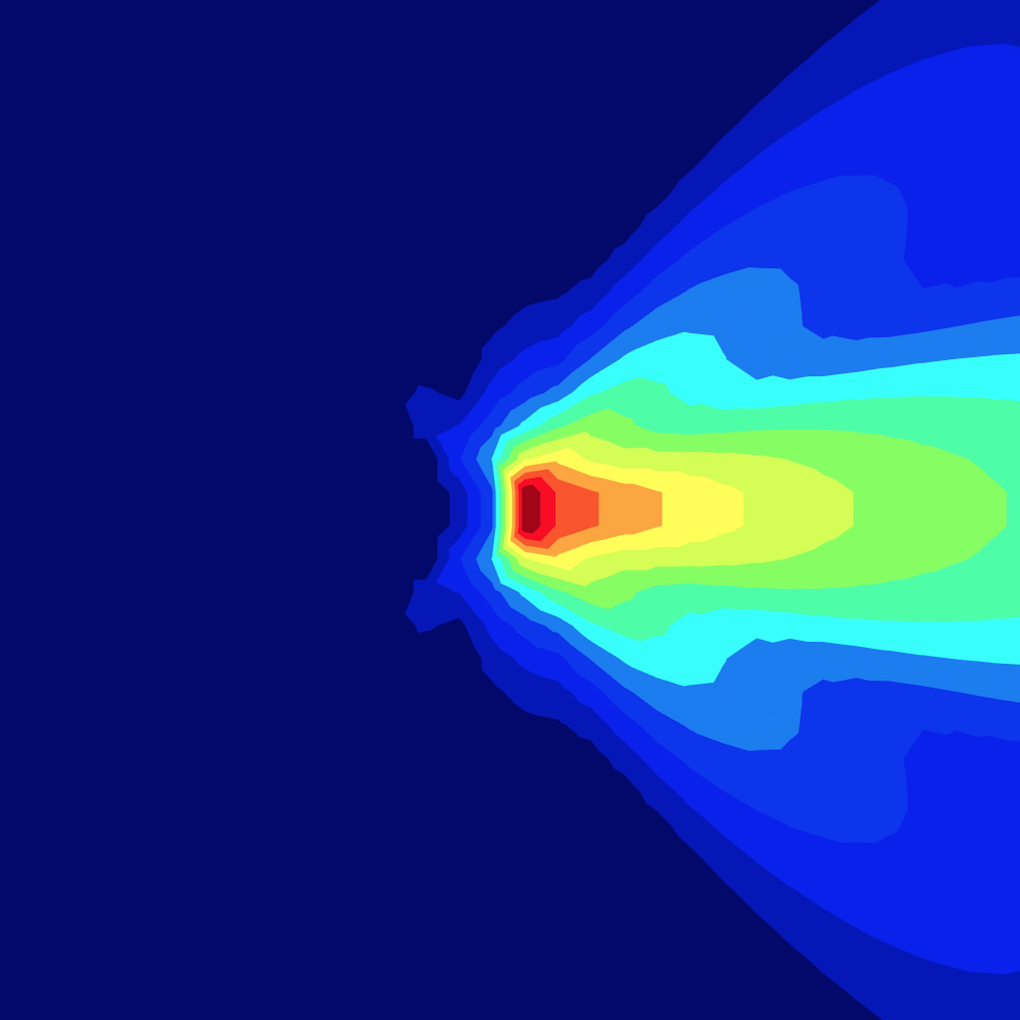
\includegraphics[scale=0.2]{archivos/130} & 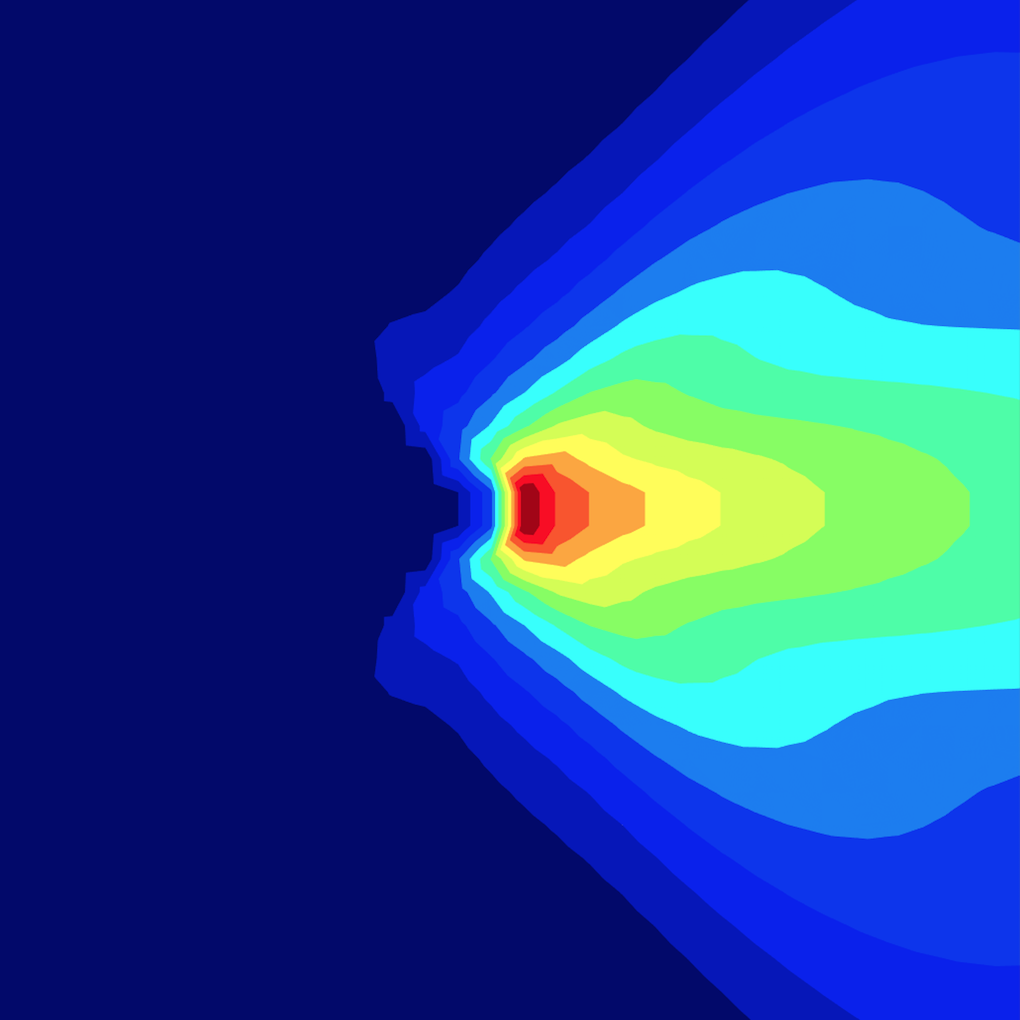
\includegraphics[scale=0.2]{archivos/160} & 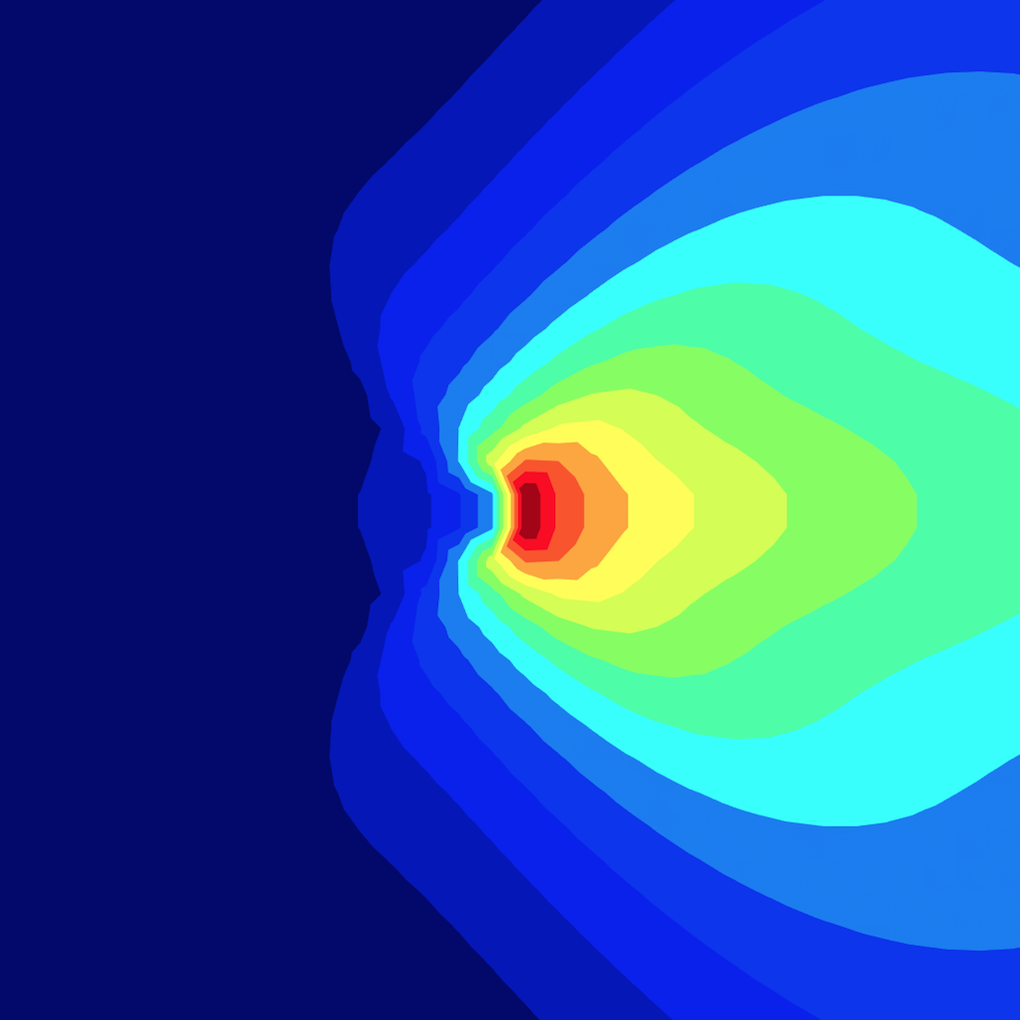
\includegraphics[scale=0.2]{archivos/190} \\
$Dist=1m \; ; \; \phi=30º$  & $Dist=1m \; ; \; \phi=60º$  & $Dist=1m \; ; \; \phi=90º$  \\
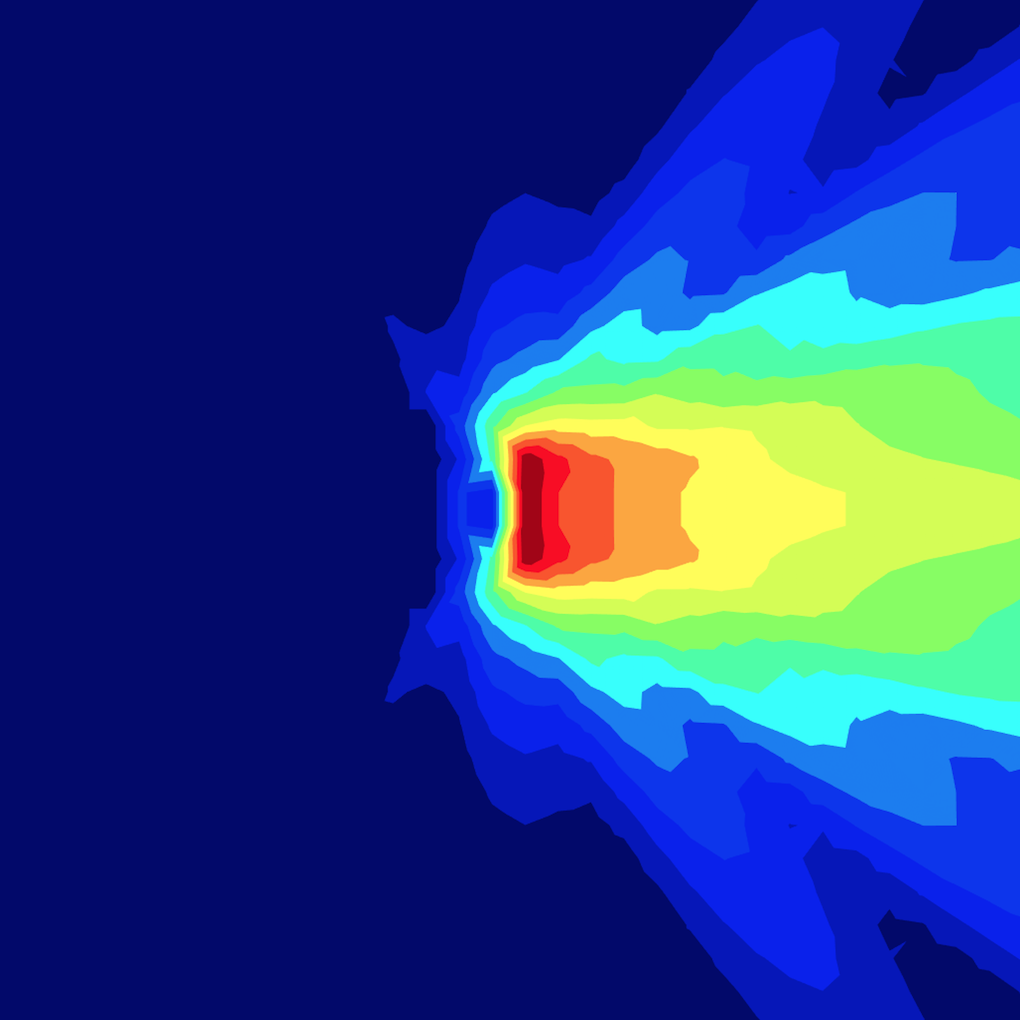
\includegraphics[scale=0.2]{archivos/230} & 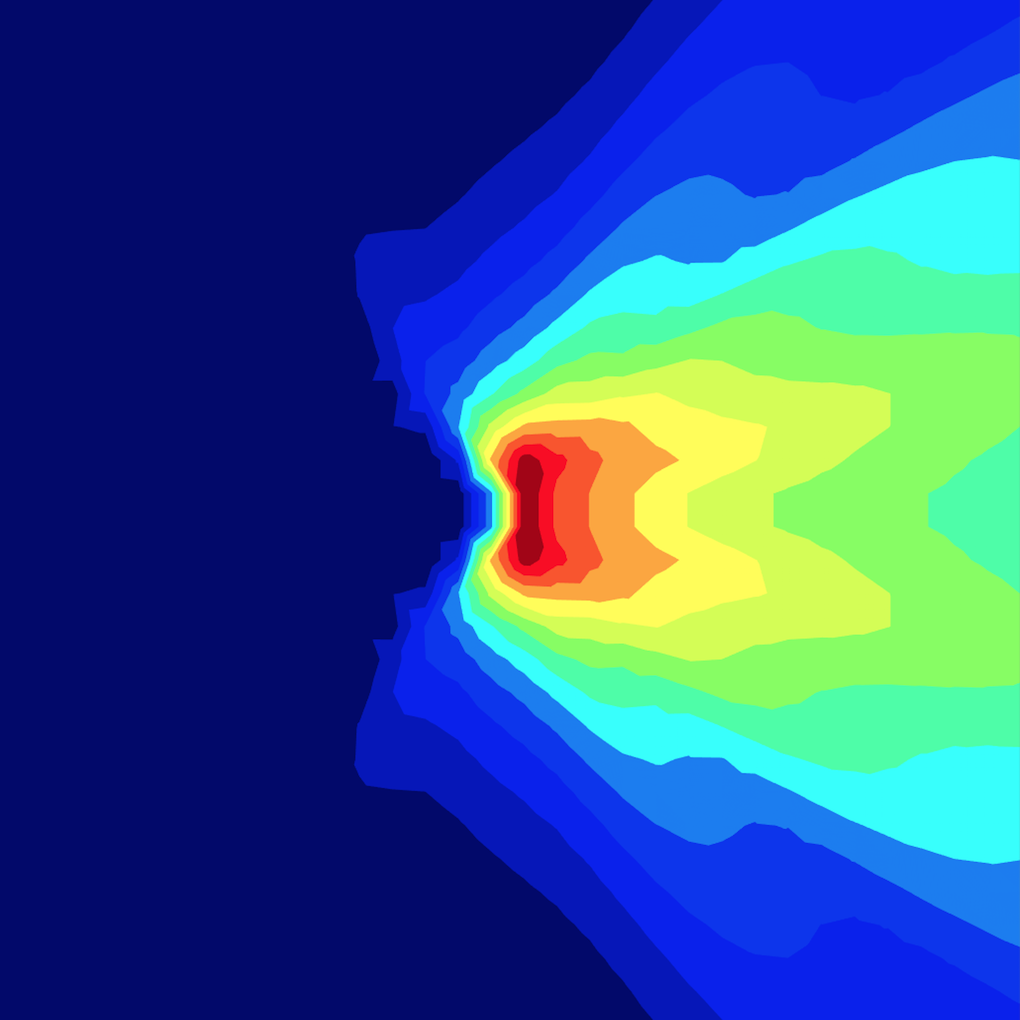
\includegraphics[scale=0.2]{archivos/260} & 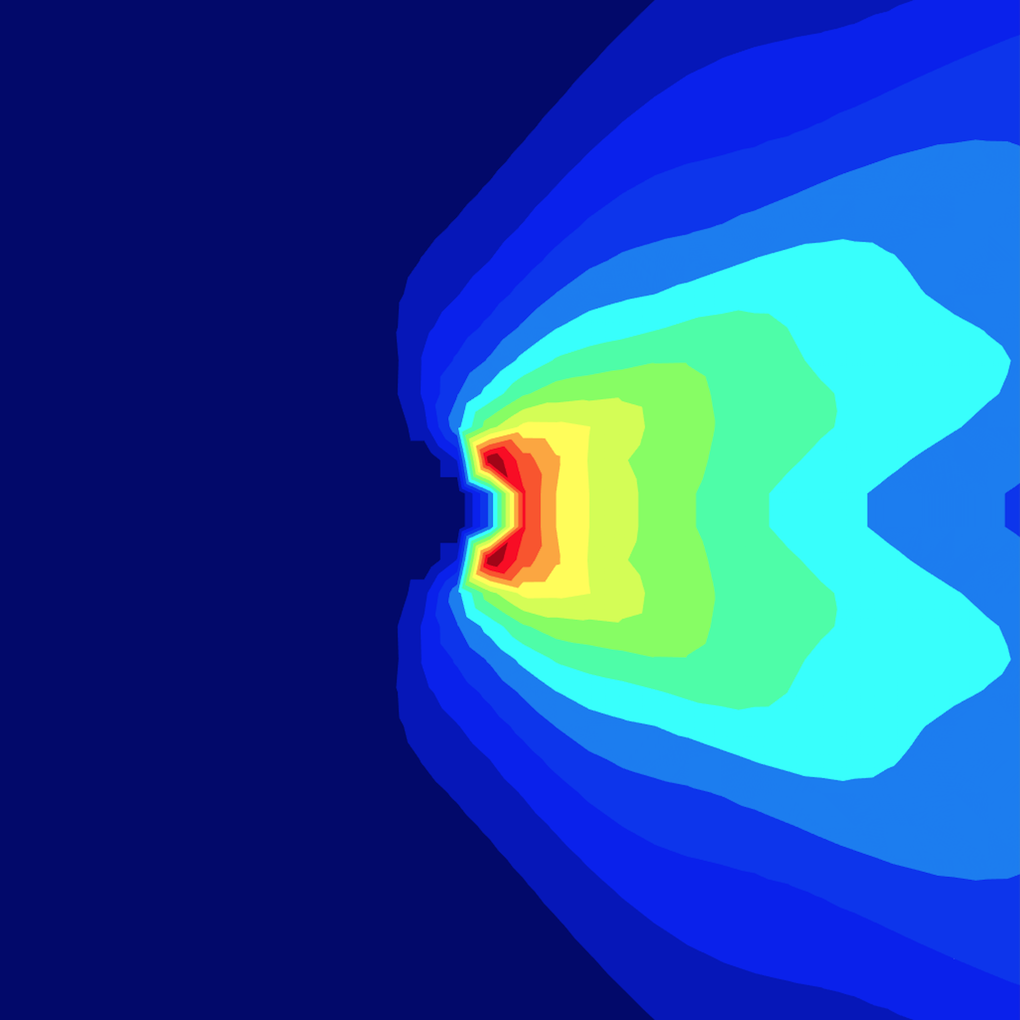
\includegraphics[scale=0.2]{archivos/290} \\
$Dist=2m \; ; \; \phi=30º$  & $Dist=2m \; ; \; \phi=60º$  & $Dist=2m \; ; \; \phi=90º$  \\
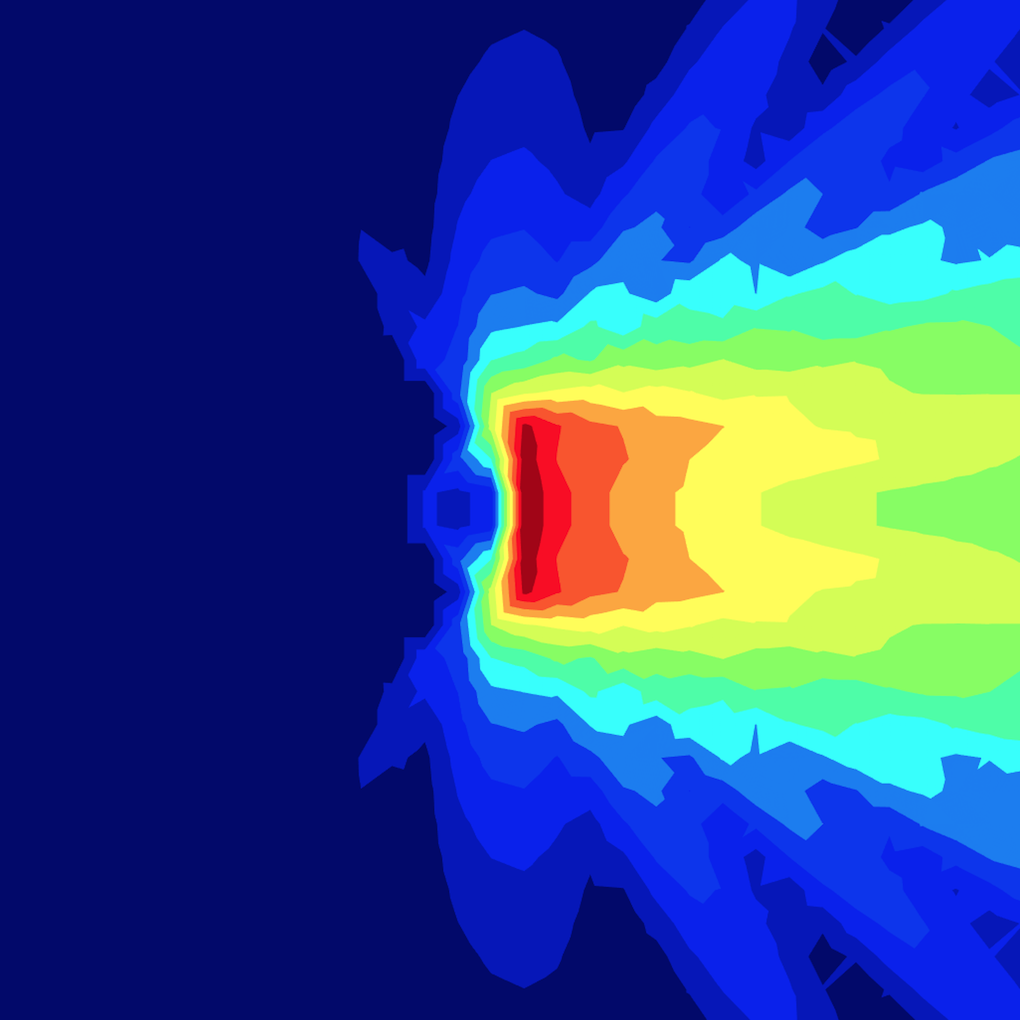
\includegraphics[scale=0.2]{archivos/330} & 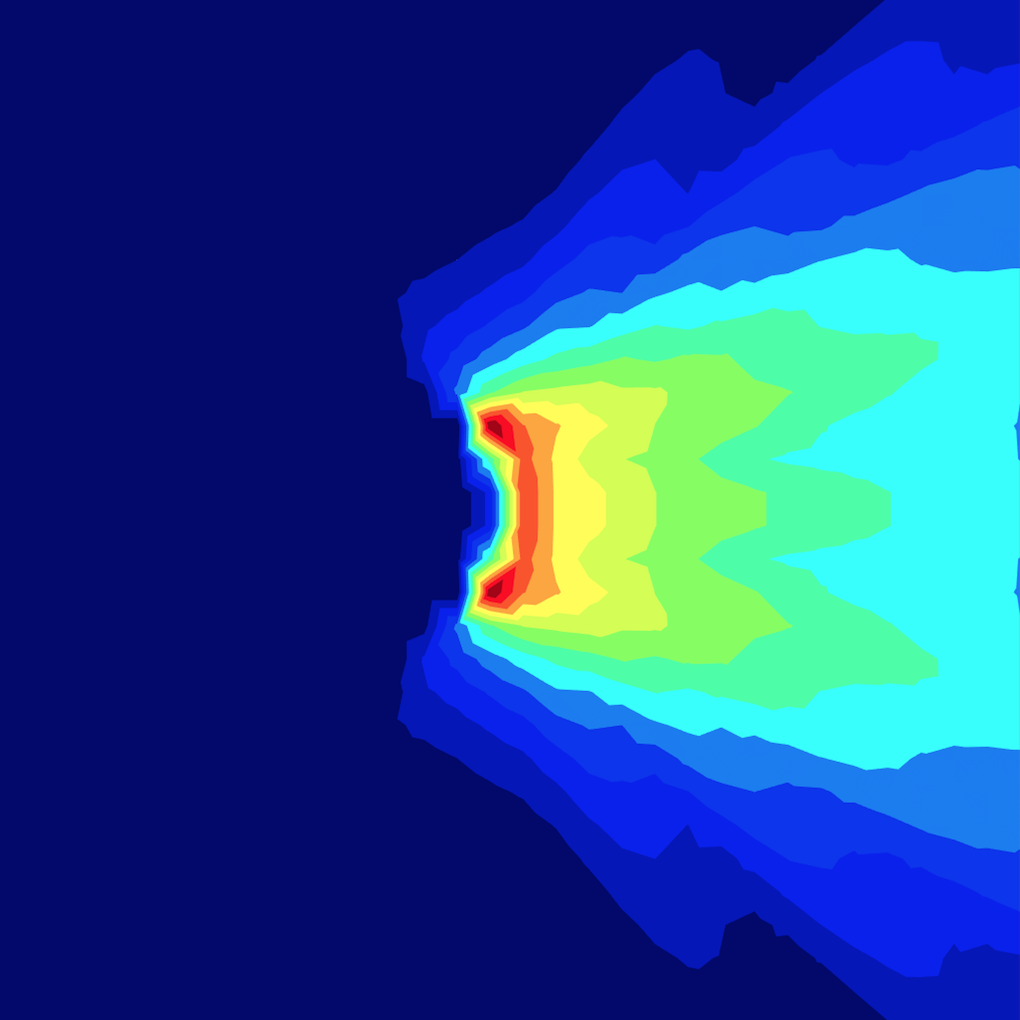
\includegraphics[scale=0.2]{archivos/360} & 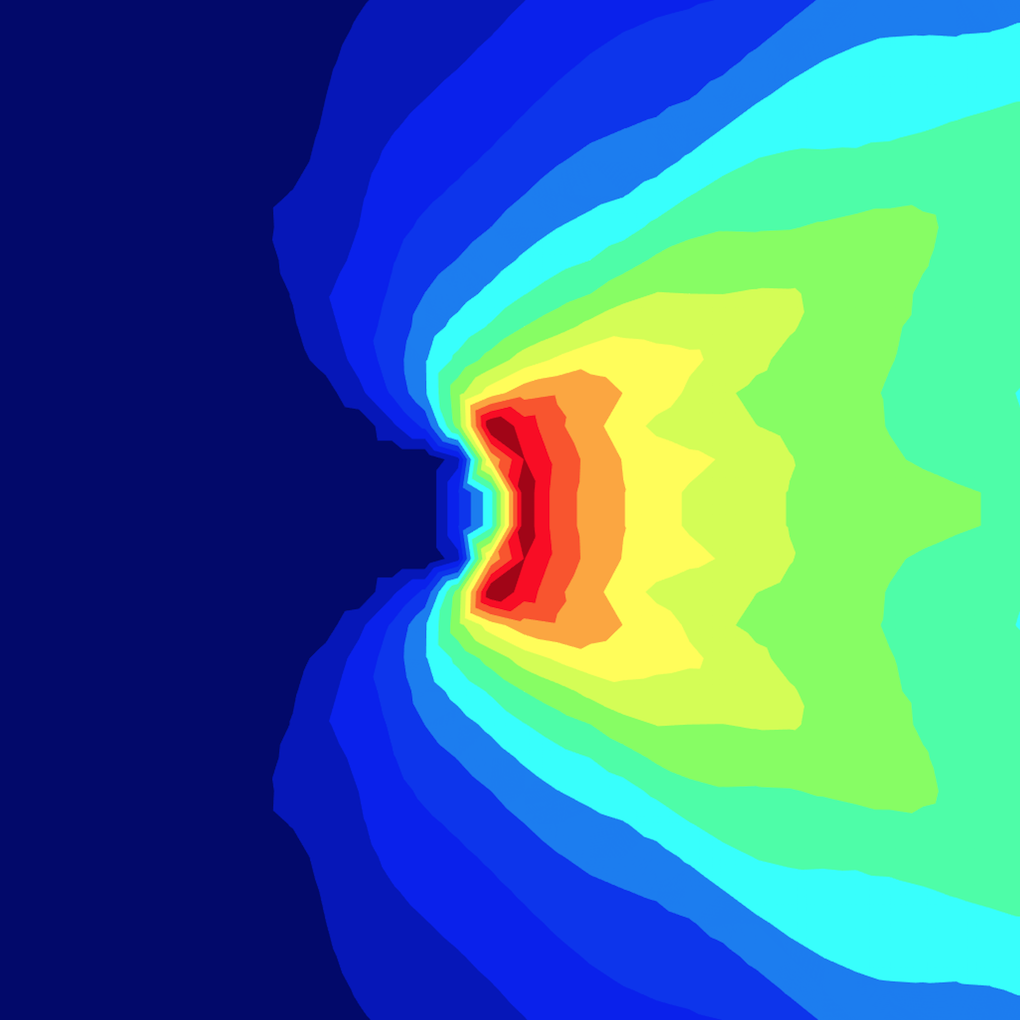
\includegraphics[scale=0.2]{archivos/390} \\
$Dist=3m \; ; \; \phi=30º$  & $Dist=3m \; ; \; \phi=60º$  & $Dist=3m \; ; \; \phi=90º$ \\
\end{tabular}
\caption{Esta es una tabla con múltiples imágenes. Útil cuando se deben mostrar varias juntas.}
\label{multiimagen} % 
\end{table}

Existe también la posibilidad de realizarlo sin tablas, con subfiguras:
\begin{lstlisting}[style=Latex-color]
\begin{figure}[h]
    \centering
    \begin{subfigure}[b]{0.4\textwidth} % Espacio horizontal ocupado por la subfigura
    	\centering
        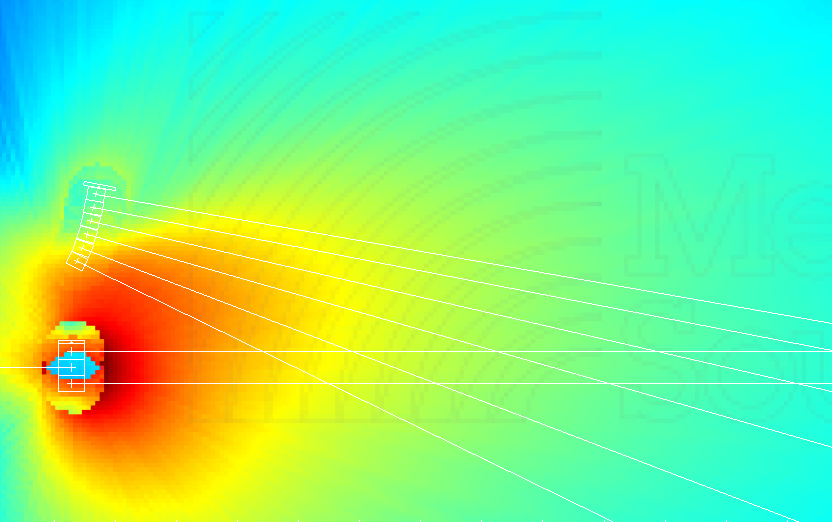
\includegraphics[width=4cm]{archivos/subs-sin} % Tamaño de la imagen
        \caption{Sin procesado.}
        \label{fig:gull}
    \end{subfigure}
    ~ % Añadir el espacio deseado, si se deja la linea en blanco la siguiente subfigura ira en una nueva linea
    \begin{subfigure}[b]{0.4\textwidth} % Espacio horizontal ocupado por la subfigura
    	\centering
        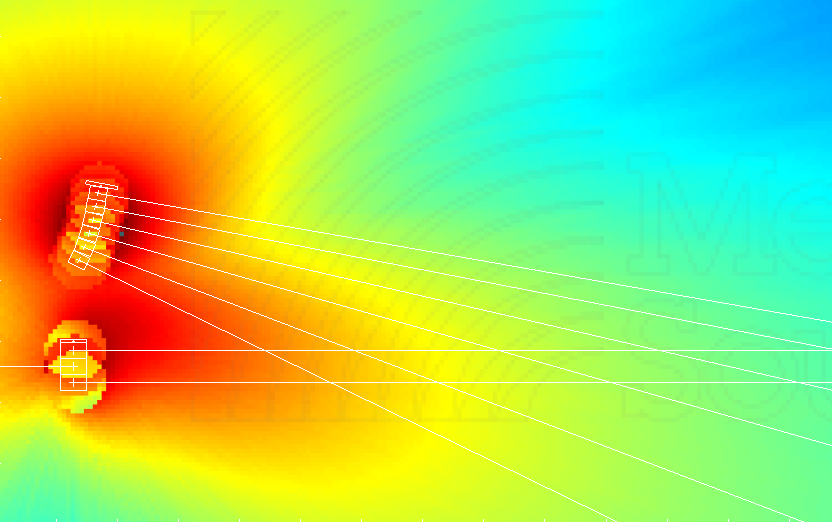
\includegraphics[width=4cm]{archivos/subs-con} % Tamaño de la imagen
        \caption{Con procesado.}
        \label{fig:tiger}
    \end{subfigure}
    \caption{Ejemplo de subfiguras}\label{sistemass}
\end{figure}
\end{lstlisting}
\begin{figure}[h]
    \centering
    \begin{subfigure}[b]{0.4\textwidth}
    	\centering
        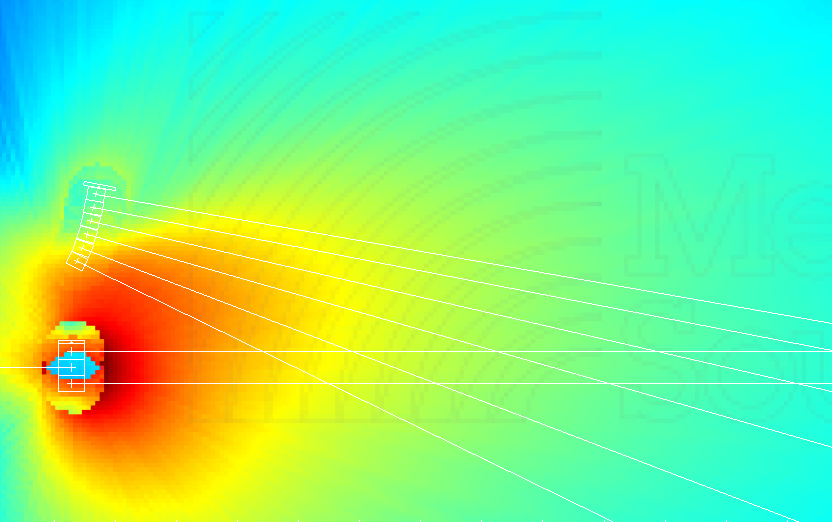
\includegraphics[width=4cm]{archivos/subs-sin}
        \caption{Sin procesado.}
        \label{fig:gull1}
    \end{subfigure}
    ~ % Añadir el espacio deseado, si se deja la linea en blanco la siguiente subfigura ira en una nueva linea
    \begin{subfigure}[b]{0.4\textwidth}
    	\centering
        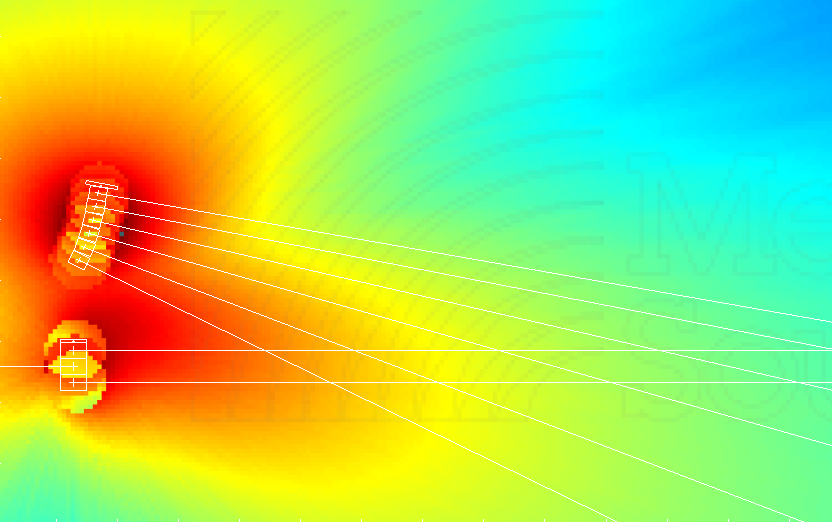
\includegraphics[width=4cm]{archivos/subs-con}
        \caption{Con procesado.}
        \label{fig:tiger1}
    \end{subfigure}
    \caption{Ejemplo de subfiguras}\label{sistemass1}
\end{figure}

\begin{figure}[h]
    \centering
    \begin{subfigure}[b]{\textwidth}
    	\centering
        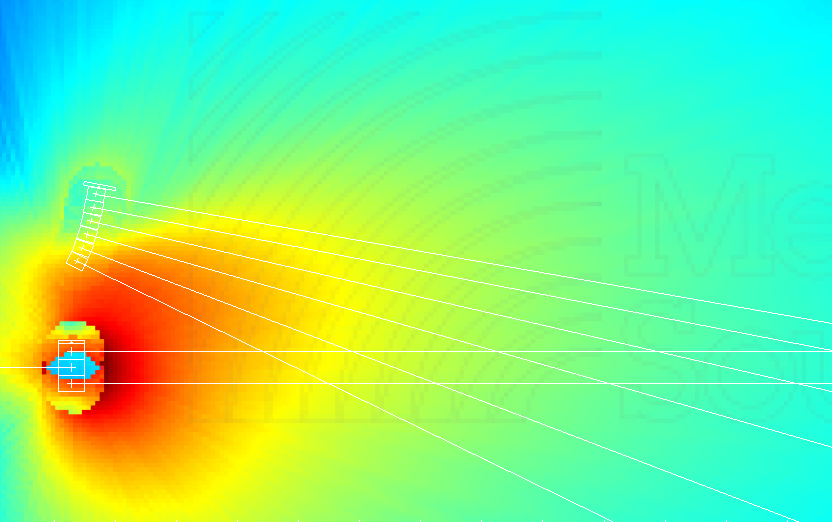
\includegraphics[width=4cm]{archivos/subs-sin}
        \caption{Sin procesado.}
        \label{fig:gull2}
    \end{subfigure}
    
    \begin{subfigure}[b]{\textwidth}
    	\centering
        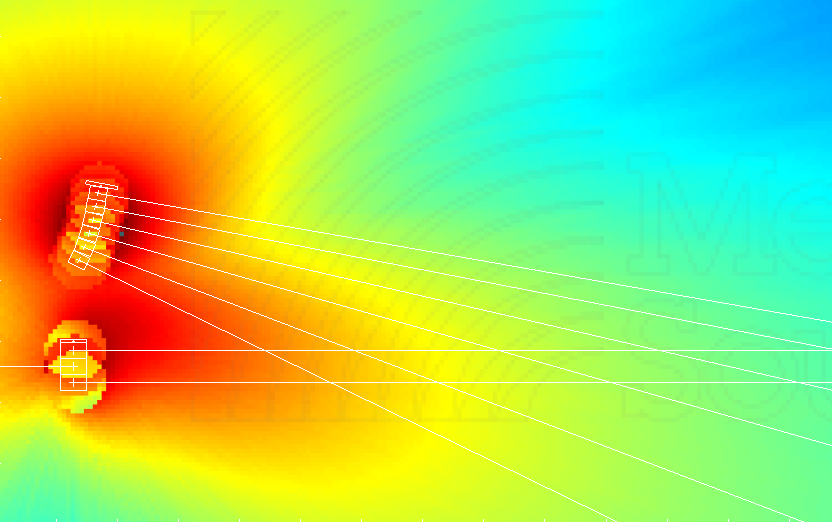
\includegraphics[width=4cm]{archivos/subs-con}
        \caption{Con procesado.}
        \label{fig:tiger2}
    \end{subfigure}
    \caption{Ejemplo de subfiguras vertical}\label{sistemass2}
\end{figure}

Si eliminas la línea '\textbackslash caption' de las subfiguras, tendrás las imágenes sin la información individual, aunque sí con la principal. Y obviamente, si eliminas el de la figura no se mostrará ninguna información.		% Plantilla: Se muestran figuras
	%%%%%%%%%%%%%%%%%%%%%%%%%%%%%%%%%%%%%%%%%%%%%%%%%%%%%%%%%%%%%%%%%%%%%%%%%
% Plantilla para escribir libros
% Universidad de A Coruña. Facultad de Informática
% Realizado por: Welton Vieira dos Santos
% Modificado: Welton Vieira dos Santos
% Contacto: welton.dosssantos@udc.es
%%%%%%%%%%%%%%%%%%%%%%%%%%%%%%%%%%%%%%%%%%%%%%%%%%%%%%%%%%%%%%%%%%%%%%%%

\chapter{Desarrollo (Con ejemplos de código)}
\label{desarrollo}

\section{Inserción de código}
A veces tendrás que insertar algún pedazo de código fuente para explicar algo relacionado con él. No sustituyas explicaciones con códigos enormes. Si pones algo de código en tu TFG que sea para demostrar algo o explicar alguna solución.

\LaTeX~te ayuda a escribir código de manera que su presentación tenga las marcas y tabulaciones propias de este tipo de texto. Para ello, debes poner el código que escribas DENTRO de un entorno  que se llama ``listings''.  La plantilla ya tiene una serie de instrucciones para incluir el paquete ``listings'' y añadirle algunos modificadores por lo que no tienes que incluirlo tú. Simplemente, mete tu código en el entorno ``lstlisting'' y ya está. Puedes indicar el lenguaje en el que está escrito el código y así \LaTeX~lo mostrará mejor. 
\\
\par En el archivo \textit{estiloscodigoprogramacion.tex} están definidos algunos lenguajes para mostrarlos con un diseño concreto, se pueden modificar para cambiar el coloreado del código, qué términos se ponen en negrita, etc.
Si se quiere profundizar más en la función ``listings'' se puede consultar su manual en \url{http://osl.ugr.es/CTAN/macros/latex/contrib/listings/listings.pdf}, aunque hay mucha información en foros y blog's que es más fácil de comprender.

\par Veamos un ejemplo en la figura \ref{C_code}:

\begin{lstlisting}[style=Latex-color]
\begin{lstlisting}[style=C, caption={ejemplo código C},label=C_code]
	#include <stdio.h>
	int main(int argc, char* argv[]) {
  	puts("Hola mundo!");
	}
\ end{lstlisting}	
\end{lstlisting}

El resultado será:
\begin{lstlisting}[style=C, caption={ejemplo código C},label=C_code]
#include <stdio.h>
// Comentario
int main(int argc, char* argv[]) {
  puts("Hola mundo!");
}
\end{lstlisting}
\vspace{1em}
\noindent\hrule
\vspace{1em}
Si lo quieres en color, está definido el estilo C-color en el archivo \textit{estiloscodigoprogramacion.tex}, con algunos parámetros para mejorar la visualización:
\begin{lstlisting}[style=Latex-color]
\begin{lstlisting}[style=C-color, caption={ejemplo código C en color},label=C_code-color]
#include <stdio.h>
// Comentario
int main(int argc, char* argv[]) {
  puts("Hola mundo!");
}
\ end{lstlisting}
\end{lstlisting}
\begin{lstlisting}[style=C-color, caption={ejemplo código C en color},label=C_code-color]
	#include <stdio.h>
	// Comentario
	int main(int argc, char* argv[]) {
  	puts("Hola mundo!");
	}
\end{lstlisting}
\vspace{1em}
\noindent\hrule
\vspace{1em}
Por supuesto, puedes mejorar esta presentación utilizando más modificadores. En la sección \ref{usos} se indican algunos detalles.

Otro ejemplo, ahora para mostrar código PHP, sería escribir en tu fichero \LaTeX~lo siguiente:
\begin{lstlisting}[style=Latex-color,numbers=none]
 \begin{lstlisting}[style=PHP, caption={ejemplo código PHP},label=PHP_code]
 /* 
Ejemplo de código en PHP para escribir tu primer programa en este lenguaje
Copia este código en tu ordenador y ejecútalo
*/
<html>
  <head>
    <title>Prueba de PHP</title>
  </head>
  <body>
    <?php echo '<p>Hola Mundo</p>'; ?> //esto lo escribe TODO el mundo
  </body>
</html>
 \ end{lstlisting}
\end{lstlisting}
 
 y el resultado es el siguiente:
 
 \begin{lstlisting}[style=PHP, caption={ejemplo código PHP},label=PHP_code,firstnumber=100]
/* 
Ejemplo de código en PHP para escribir tu primer programa en este lenguaje. Copia este código en tu ordenador y ejecútalo
*/
 <html>
  <head>
    <title>Prueba de PHP</title>
  </head>
  <body>
    <?php echo '<p>Hola Mundo</p>'; ?> //esto lo escribe TODO el mundo
  </body>
</html>
 \end{lstlisting}
 \vspace{1em}
\noindent\hrule
\vspace{1em}
 O también en color: 
 \begin{lstlisting}[style=PHP-color, caption={ejemplo código PHP},label=PHP_code2]
/* 
Ejemplo de código en PHP para escribir tu primer programa en este lenguaje. Copia este código en tu ordenador y ejecútalo
*/
 <html>
  <head>
    <title>Prueba de PHP</title>
  </head>
  <body>
    <?php echo '<p>Hola Mundo</p>'; ?> //esto lo escribe TODO el mundo
  </body>
</html>
 \end{lstlisting}
 
 Observa cómo \LaTeX~ha puesto los comentarios en gris y ajustado el código para que se muestre más claro.
\vspace{1em}
\noindent\hrule
\vspace{1em}
 A continuación se muestran otros ejemplos:
 \begin{lstlisting}[style=Matlab-color, caption={ejemplo código Matlab en color},label=Matlab_code]
%% Code sections are highlighted.
% System command are supported...
!touch testFile.txt
A = [1, 2, 3;... %... as is line continuation.
     4, 5, 6];
fid = fopen('testFile.text', 'w');
for k=1:10
  fprintf(fid, '%6.2f \n', k)
end
x=1; %% this is just a comment, not the start of a section
% Context-sensitive keywords get highlighted correctly...
p = properties(person); %(here, properties is a function)
x = linspace(0,1,101);
y = x(end:-1:1);
% ... even in nonsensical code.
]end()()(((end while {    end    )end ))))end (end
%{
    block comments are supported
%} even
runaway block comments are
\end{lstlisting}

\begin{lstlisting}[style=Matlab, caption={ejemplo código Matlab en blanco y negro},label=Matlab_codebn]
%% Code sections are highlighted.
% System command are supported...
!touch testFile.txt
A = [1, 2, 3;... %... as is line continuation.
     4, 5, 6];
fid = fopen('testFile.text', 'w');
for k=1:10
  fprintf(fid, '%6.2f \n', k)
end
x=1; %% this is just a comment, not the start of a section
% Context-sensitive keywords get highlighted correctly...
p = properties(person); %(here, properties is a function)
x = linspace(0,1,101);
y = x(end:-1:1);
% ... even in nonsensical code.
]end()()(((end while {    end    )end ))))end (end
%{
    block comments are supported
%} even
runaway block comments are
\end{lstlisting}
\newpage
\begin{lstlisting}[style=Python-color, caption={ejemplo código Python en color}]
class Example (object):
    def __init__ (self, account, password):
        """e.g. account  = 'bob@example.com/test'
                password = 'bigbob'
        """

        reg = telepathy.client.ManagerRegistry()
        reg.LoadManagers()

        # get the gabble Connection Manager
        self.cm = cm = reg.GetManager('gabble')

        # get the parameters required to make a Jabber connection
        # begin ex.basics.dbus.language-bindings.python.methods.call
        cm[CONNECTION_MANAGER].RequestConnection('jabber',
            {
                'account':  account,
                'password': password,
            },
            reply_handler = self.request_connection_cb,
            error_handler = self.error_cb)
        # end ex.basics.dbus.language-bindings.python.methods.call
\end{lstlisting}

\begin{lstlisting}[style=Python, caption={ejemplo código Python en blanco y negro}]
class Example (object):
    def __init__ (self, account, password):
        """e.g. account  = 'bob@example.com/test'
                password = 'bigbob'
        """

        reg = telepathy.client.ManagerRegistry()
        reg.LoadManagers()

        # get the gabble Connection Manager
        self.cm = cm = reg.GetManager('gabble')

        # get the parameters required to make a Jabber connection
        # begin ex.basics.dbus.language-bindings.python.methods.call
        cm[CONNECTION_MANAGER].RequestConnection('jabber',
            {
                'account':  account,
                'password': password,
            },
            reply_handler = self.request_connection_cb,
            error_handler = self.error_cb)
        # end ex.basics.dbus.language-bindings.python.methods.call
\end{lstlisting}

\section{Usos y personalización}
\label{usos}

El texto que acompaña al código puedes incluirlo o no, también puedes decidir si el texto va numerado o no. A continuación se muestra como:
\begin{lstlisting}[style=Latex-color]
	% Con esta línea el código no tendrá título
	\begin{lstlisting}[style=Python]
		micodigo
	\ end{lstlisting}
\end{lstlisting}

\begin{lstlisting}[style=Python]
	micodigo
\end{lstlisting}
\vspace{1em}
\noindent\hrule
\vspace{1em}
\begin{lstlisting}[style=Latex-color]
	% Con esta línea el código tendrá el título abajo
	\begin{lstlisting}[style=Python, caption={Ejemplo de título abajo},captionpos=b]
		micodigo
	\ end{lstlisting}
\end{lstlisting}

\begin{lstlisting}[style=Python,caption={Ejemplo de título abajo},captionpos=b]
	micodigo
\end{lstlisting}
\vspace{1em}
\noindent\hrule
\vspace{1em}
\begin{lstlisting}[style=Latex-color]
	% Con esta línea el código tendrá título no numerado
	\begin{lstlisting}[style=Python, title={Ejemplo de título no numerado}]
		micodigo
	\ end{lstlisting}
\end{lstlisting}

\begin{lstlisting}[style=Python,title={Ejemplo de título no numerado}]
	micodigo
\end{lstlisting}
\vspace{1em}
\noindent\hrule
\vspace{1em}
\begin{lstlisting}[style=Latex-color]
	% Con esta línea el código no tendrá las líneas numeradas
\begin{lstlisting}[style=Python,numbers=none, title={Ejemplo de código sin número de líneas}]
	micodigo
	sin
	número
	de
	líneas
\ end{lstlisting}
\end{lstlisting}

\begin{lstlisting}[style=Python,numbers=none,title={Ejemplo de código sin número de líneas}]
		micodigo
		sin
		número
		de
		líneas
\end{lstlisting}

\section{Importar archivos fuente}

Existe la posibilidad de importar un archivo de código en lugar de copiar su contenido y pegarlo en \LaTeX.

Para realizarlo debes escribir:

\begin{lstlisting}[style=Latex-color]
\lstinputlisting[style=C++-color,caption={Archivo C++ importado}]{archivos/ejemplos/holamundo.cpp}	
\end{lstlisting}

Y se importará con el formato establecido entre los '[ ]':
\newpage
\lstinputlisting[style=C++-color,caption={Archivo C++ importado}]{archivos/ejemplos/holamundo.cpp}

A continuación se muestran otros ejemplos

\begin{lstlisting}[style=Latex-color]
\lstinputlisting[style=Python-color,caption={Archivo Py importado},label=importado_py]{archivos/ejemplos/holamundo.py}	
\end{lstlisting}

\lstinputlisting[style=Python-color,caption={Archivo Py importado},label=importado_py2]{archivos/ejemplos/holamundo.py}	

\begin{lstlisting}[style=Latex-color]
\lstinputlisting[style=Matlab-color,caption={Archivo Matlab importado},label=importado_m]{archivos/ejemplos/holamundo.m}	
\end{lstlisting}

\lstinputlisting[style=Matlab-color,caption={Archivo Matlab importado},label=importado_m]{archivos/ejemplos/holamundo.m}

Ejemplo de una tablas:

\begin{table}[H]\centering
	\scalebox{0.94}{
	\setlength{\extrarowheight}{3pt}
		\begin{tabular}{rm{1.85cm}m{5cm}m{4cm}m{3.6cm}}
		\hline
			  &       & 3 Puntos & 2 Puntos & 1 Punto \\
		\hline \hline
		\multirow{12}{*}{\rotatebox[origin=rB]{90}{Ejemplo de Multifila}}    & Ortografía & Impecable & Hasta 4 errores & Más de 4 errores. \\ \cline{3-5}
			& Claridad & Todo el documento es lógico. & Una sección requiere mejor redacción. & Más de una sección requiere mejor redacción. \\ \cline{3-5}
			& Extensión & La práctica comprende entre 4 y 10 hojas. (Sin apéndices.) &       & La práctica es inferior a 4 hojas o superior a 10. (Sin apéndices.) \\ \cline{3-5}
			& Completez & La práctica cubre todas las solicitudes de trabajo. & Falta una solicitud de trabajo. & Falta más de una solicitud de trabajo. \\ \cline{3-5}
			& Gráficas & Gráficas con curvas identificadas, ejes y leyendas explicativas con unidades, y pie de figura. & Una gráfica está mal presentada. & Más de una gráfica está mal presentada. \\ \cline{3-5}
			& Diagramas/ Fotos & Claros. Ayudan a entender lo escrito. & Son poco claros. & Sólo las incluye. \\ \cline{3-5}
		7)    & Título & Corto, descriptivo y acertado. & Necesita cambios ligeros. & Requiere cambios mayores. \\ \cline{3-5}
		8)    & Resumen & Cubre brevemente por completo el trabajo realizado. & Puede redactarse mejor. & Deja puntos clave sin describir. \\ \cline{3-5}
		9)    & Introducción & Introduce clara y brevemente el trabajo realizado. & Introduce al trabajo realizado pero divaga en otros temas. & Requiere cambios mayores. \\ \cline{3-5}
		10)   & Metodología & Describe claramente lo realizado, materiales, equipo y disposición. Explica los cuidados tomados al realizar medidas y toma de datos. & Describe lo realizado en la practica y explica la realización de las medidas y la toma de datos. & Describe materiales y equipo empleado. \\ \cline{3-5}
		11)   & Resultados y Discusión & Resultados claros. Amplia explicación del significado e implicación física. Además, se comparan con otras fuentes de investigación. & Resultados con explicación de su significado físico. & Requiere mejoras en redacción y presentación. \\ \cline{3-5}
		12)   & Conclusión & Breve y cubre por completo lo realizado por el estudiante, sin divagar. & No cubre por completo lo realizado por el estudiante. & Requiere cambios mayores. \\ \cline{3-5}
		13)   & Referencias & Al menos 5 referencias, correctamente redactadas y citadas en el reporte. & Al menos 3 referencias, correctamente redactadas y citadas en el reporte.  & Al menos 1 referencia, correctamente citada.  \\ \cline{3-5}
		\hline
		\end{tabular}
	}
	\label{tab:Rubrica}
\end{table}

Ejemplo II

\begin{table}[H]\centering
  \begin{tabularx}{\textwidth}{XXXm{6.0cm}}\toprule
    Nombre & GPU  & Licencia & Descripción		\\		\midrule\midrule
    Abalone & Sí & Libre & Pliegue de proteínas y simulaciones de biomoléculas. \\
    AMBER & Sí & De Pago & Familia de campos de fuerza para dinámica molecular. \\
    CHARMM & No & Comercial & Conjunto de campos de fuerza y simulaciones de biomoléculas. \\
    DL\_POLY & Sí & Libre & Dinámica molecular en paralelo para uso general. \\
    fold.it & No & Libre & Predicción de estructura. Plegamiento molecular. \\
    GROMMACS & Sí & Libre & Simulaciones de Alto Rendimiento. \\ 
    LAMMPS & Sí & Libre & Potenciales sistemas blandos, granulares, y de estado sólido. \\
    NAMD & Sí & Libre & Computación en paralelo para dinámica molecular. \\
    TeraChem & Sí & Privado & Ab initio de alto rendimiento, optimizada para CUDA. \\
    TINKER & No & Libre & Herramientas de software para el diseño molecular. \\		\bottomrule
  \end{tabularx}
  \caption{Algunos programas de simulación en dinámica molecular.}\label{tab:ProgramasDM}
\end{table}EndFragment

Ejemplo III

\begin{table}[htbp]\centering
  \begin{tabular}{|r|c|c|c|c|c|c|c|c|c|c|c|}\hline
      & \multicolumn{5}{c|}{2017}      & \multicolumn{6}{c|}{2018} \\ \cline{2-12}
      & Ago & Sep & Oct & Nov & Dic & Ene & Feb & Mar & Abr & May  & Jun \\ \hline
    \makecell[r]{Revisión \\ Bibliográfica} & \cclg & \cclg & \cclg & \cclg &	&	&	&	&	&	&  \\ \hline
    \makecell[r]{Escritura \\ del Protocolo} &	&	& \cclg &	&	&	&	&	&	&	&  \\ \hline
    \makecell[r]{Tema \\ A} & &	&	& \cclg & \cclg & \cclg &	&	&	&	&  \\ \hline
    \makecell[r]{Tema \\ B} & &	&	&	& \cclg & \cclg & \cclg &	&	&	&  \\ \hline
    \makecell[r]{Tema \\ C} & &	&	&	& \cclg & \cclg & \cclg &	&	&	&  \\ \hline
    \makecell[r]{Tema \\ D} & &	&	&	&	& \cclg & \cclg & \cclg &	&	&  \\ \hline
    \makecell[r]{Tema \\ E} & &	&	&	&	&	& \cclg & \cclg & \cclg &	&  \\ \hline
    Escritura de Tesis & &	&	&	&	&	& \cclg & \cclg & \cclg & \cclg &  \\ \hline
    Escritura de Artículo & &	&	&	&	&	&	&	& \cclg & \cclg & \cclg \\ \hline
    Defensa & &	&	&	&	&	&	&	&	&	& \cclg \\ \hline
  \end{tabular}
  \caption{Cronograma de Actividades.}
  \label{tab:CronoAct}
\end{table}
		% Plantilla: Se muestran listados
	%%%%%%%%%%%%%%%%%%%%%%%%%%%%%%%%%%%%%%%%%%%%%%%%%%%%%%%%%%%%%%%%%%%%%%%%%
% Plantilla para escribir libros
% Universidad de A Coruña. Facultad de Informática
% Realizado por: Welton Vieira dos Santos
% Modificado: Welton Vieira dos Santos
% Contacto: welton.dosssantos@udc.es
%%%%%%%%%%%%%%%%%%%%%%%%%%%%%%%%%%%%%%%%%%%%%%%%%%%%%%%%%%%%%%%%%%%%%%%%

\chapter{Resultados (Con ejemplos de gráficos)}
\label{resultados}

\section{Diagramas}
Gracias al paquete \textit{Tikz} se pueden incluir multitud de medios gráficos, diagramas, capas sobre imágenes, etc.
Existen múltiples formas de realizarlo, para ello es recomendable consultar la guía de iniciación disponible aquí: \url{http://cremeronline.com/LaTeX/minimaltikz.pdf} y también el manual completo disponible aquí: \url{http://osl.ugr.es/CTAN/graphics/pgf/base/doc/pgfmanual.pdf}.
\\
\par A continuación se muestran algunos ejemplos. Revisa el archivo .tex para ver cómo se utilizan.
\\
\par Imagen a la que se le ha añadido cuadros y texto desde latex:
\begin{figure}[ht]
\centering	
\resizebox{0.6\textwidth}{!}{%
\begin{tikzpicture}[x=39, y=47]%X,Y -> Corrección de coordenadas, según tamaño y posición de la imagen
    \node[anchor=south west,inner sep=0] (image) at (0,0) {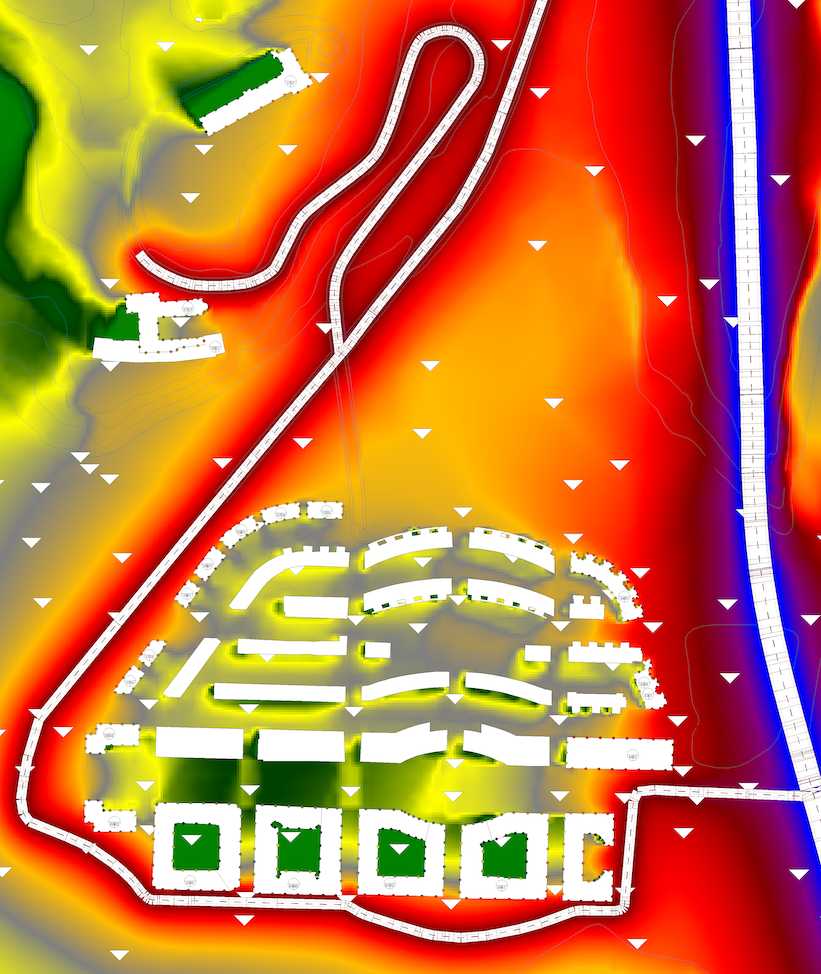
\includegraphics[width=0.9\textwidth]{archivos/mapadia}};
    % Imprimir coordenadas
    \begin{scope}[x={(image.south east)},y={(image.north west)}]
        \draw[help lines,xstep=.1,ystep=.1] (0,0) grid (1,1);
        \foreach \x in {0,1,...,9} { \node [anchor=north] at (\x/10,0) {\x}; }
        \foreach \y in {0,1,...,9} { \node [anchor=east] at (0,\y/10) {\y}; }
    \end{scope}
    % Residencias 1
    \draw[Caja1] (6.8,2) rectangle (8.3,4.5);
    \node[Texto2] at (6.8,2) {\textbf{Residencias 1}};
    % Residencias 2
    \draw[Caja1] (1,0.6) rectangle (7.6,1.8);
    \node[Texto2] at (1,0.6) {\textbf{Residencias 2}};
    % Residencias 3
    \draw[Caja1,rotate around={-45:(2.6,3.6)}] (2.6,3.6) ellipse (1cm and 3.1cm);
    \node[Texto2] at (1.2,2.1) {\textbf{Residencias 3}};
    % Hospital
    \draw[Caja1] (1,6) rectangle (3,7);
    \node[Texto2] at (1,6) {\textbf{Hospital}};
    % Colegio
    \draw[Caja1] (2.3,8.5) rectangle (3.9,9.5);
    \node[Texto2] at (2.3,8.5) {\textbf{Colegio}};
    % Numeros de edificios
    \node[Texto3,font=\tiny] at (7.5,4) {\textbf{1}};
    \node[Texto3,font=\tiny] at (7.9,2.9) {\textbf{2}};
    \node[Texto3,font=\tiny] at (7.7,2.3) {\textbf{3}};
    \node[Texto3,font=\tiny] at (7.2,1.2) {\textbf{4}};
    \node[Texto3,font=\tiny] at (6.2,1.2) {\textbf{5}};
    \node[Texto3,font=\tiny] at (4.9,1.2) {\textbf{6}};
    \node[Texto3,font=\tiny] at (3.6,1.2) {\textbf{7}};
    \node[Texto3,font=\tiny] at (2.4,1.2) {\textbf{8}};
    \node[Texto3,font=\tiny] at (1.5,1.7) {\textbf{9}};
    \node[Texto3,font=\tiny] at (1.5,2.5) {\textbf{10}};
    \node[Texto3,font=\tiny] at (1.5,3) {\textbf{11}};
    \node[Texto3,font=\tiny] at (1.8,3.4) {\textbf{12}};
    \node[Texto3,font=\tiny] at (2.2,3.8) {\textbf{13}};
    \node[Texto3,font=\tiny] at (2.5,4.2) {\textbf{14}};
    \node[Texto3,font=\tiny] at (3,4.5) {\textbf{15}};
    \node[Texto3,font=\tiny] at (3.4,4.8) {\textbf{16}};
    \node[Texto3,font=\tiny] at (4,4.8) {\textbf{17}};
    % Nombres de carreteras
    \node[Texto3] at (9.2,7) {\textbf{A-7}};
    \node[Texto3] at (9,1.8) {\textbf{N-1}};
    \node[Texto3] at (4,8) {\textbf{N-2}};
\end{tikzpicture}
}
\end{figure}

En muchas ocasiones es necesario realizar un diagrama de bloques, más abajo se muestra un ejemplo de ello. En la red hay multitud de ejemplos que pueden ser fácilmente modificables para un fin concreto, como por ejemplo en esta web: \url{http://www.texample.net/tikz/examples/tag/block-diagrams/}.
\begin{figure}[ht]
\centering 
\begin{tikzpicture}[node distance=2cm, auto]
	% Cuadros
	\node (pc) [rectvioleta,text width=3cm] {Ordenador{\\}\small{Software: ARTA} \par};
	\node (sound) [rectamarillo, below of=pc, text width=4cm] {Tarjeta de sonido {\\}Tascam US-144MKII \par};
	\node (nexus) [rectverde, right of=sound,xshift=6cm, text width=8cm] { Amplificador/Adaptador de impedancia{\\}DIY\par };
	\node (acel) [rectnaranja, below of=nexus,text width=3cm,xshift=0cm]{\small Acelerómetro {\\}Brüel {\&} Kjær TYPE 4514B-002 \par};
	\node (micro) [rectnaranja, below of=sound,text width=3cm,xshift=0cm]{\small Micrófono {\\}Behringer ECM8000 \par};
	\node (excit) [rectnaranja, below of=acel,text width=3cm,xshift=2cm]{\small Excitador \par};
	\node(barra) [romborosa, below of=acel,xshift=-3.1cm]{\small Barra \par};
	% Flechas
	\draw[arrow] (pc) -- (sound);
	\draw[arrow] (sound) -- (pc);
	\draw[arrow] (nexus) -- (sound);
	\draw[arrow] (excit) -- (barra.east);
	\draw[arrow] (micro) -- (sound);
	\draw[arrow] (barra.west) -- (0,-6)-- (micro.south);
	\draw[arrow] (barra.west) -- (3.4,-4)--(acel.west);
 	\draw[arrow] (acel) -- (nexus);	
\end{tikzpicture}
\caption{Diagrama realizado en latex con Tikz.}
\label{fig:blockcv}
\end{figure}



\section{Gráficas}

Existen múltiples formas de generar gráficas para latex. Hay disponibles herramientas como GeoGebra que dispone de la utilidad para exportar los gráficos en formato Tkiz. También funciones para Matlab que genera las gráficas que muestra habitualmente pero en código para Tkiz.

La forma más simple, aunque no sencilla cuando abarca muchos datos es la siguiente:

\begin{lstlisting}[style=Latex-color]
\begin{figure}[ht]
\centering
	\begin{tikzpicture}
  		\begin{axis}
  			[ymin=0,ymax=5, % Límites del eje y
  			xmin=0,xmax=6,  % Límites del eje x
  			ylabel= eje Y, 	% Nombre del eje y
    		xlabel= eje X]  % Nombre del eje x
    		\addplot+[smooth] coordinates % Une los puntos curva suavizada
      		{(0,0) (1,2) (2,3 (4,3))}; % Puntos de la gráfica
  		\end{axis}
	\end{tikzpicture}
\caption{Gráfica sencilla.}
\end{figure}
\end{lstlisting}

El resultado es el siguiente:
\\
\begin{figure}[ht]
\centering
	\begin{tikzpicture}
  		\begin{axis}
  			[ymin=0,ymax=5, 
  			xmin=0,xmax=6,
  			ylabel= eje Y,
    		xlabel= eje X]
    		\addplot+[smooth] coordinates
      		{(0,0) (1,2) (2,3) (4,3)};
  		\end{axis}
	\end{tikzpicture}
\caption{Gráfica sencilla.}
\end{figure}
\FloatBarrier
\vspace{1em}
\noindent\hrule
\vspace{1em}
Otro ejemplo es la gráfica de barras:
\begin{lstlisting}[style=Latex-color]
\begin{figure}[ht]
\centering
\begin{tikzpicture}
	\begin{axis}[
	    ybar=12pt,
	    ymin=0,ymax=150,
	    xtick=data,
	    enlarge x limits={abs=2cm},
	    symbolic x coords={rubio, moreno},
	    bar width = 20pt,
	    ylabel= número,
	    xlabel= color de pelo,
	        ytick align=outside,
	        ytick pos=left,
	        major x tick style = transparent,
	        legend style={at={(0.04,0.96)},anchor=north west, font=\footnotesize, legend cell align=left,},
	        ]
	    \addplot[ybar,fill=blue, area legend] coordinates {
	        (rubio,20)
	        (moreno,100)};
	    \addplot[ybar,fill=purple, area legend] coordinates {
	        (rubio,110)
	        (moreno,105)};
	 \legend{Chicos, Chicas}
	\end{axis}
\end{tikzpicture}
\caption{Gráfica barras.}
\end{figure}
\end{lstlisting}

El resultado es el siguiente:

\begin{figure}[ht]
\centering
\begin{tikzpicture}
	\begin{axis}[
	    ybar=12pt,
	    ymin=0,ymax=150,
	    xtick=data,
	    enlarge x limits={abs=2cm},
	    symbolic x coords={rubio, moreno},
	    bar width = 20pt,
	    ylabel= número,
	    xlabel= color de pelo,
	        ytick align=outside,
	        ytick pos=left,
	        major x tick style = transparent,
	        legend style={at={(0.04,0.96)},anchor=north west, font=\footnotesize, legend cell align=left,},
	        ]
	    \addplot[ybar,fill=blue, area legend] coordinates {
	        (rubio,20)
	        (moreno,100)};
	    \addplot[ybar,fill=purple, area legend] coordinates {
	        (rubio,110)
	        (moreno,105)};
	 \legend{Chicos, Chicas}
	\end{axis}
\end{tikzpicture}
\caption{Gráfica barras.}
\end{figure}
\FloatBarrier
\section{Importados de Matlab}

Gracias a la herramienta \textit{matlab2tikz} (\url{https://es.mathworks.com/matlabcentral/fileexchange/22022-matlab2tikz-matlab2tikz}) se pueden exportar las gráficas de cualquier tipo de Matlab a latex.
Después de incluir los archivos de \textit{matlab2tikz} se debe escribir una llamada después de crear la figura tal que:

\begin{lstlisting}[style=Matlab-color,caption={Ejemplo de llamada a matlab2tikz}]
fig = plot(x,y);
matlab2tikz('figurehandle',fig,'NombreArchivo.tex','height','5cm','width','13.5cm','strict',true,'showHiddenStrings',true,'showInfo',false)
\end{lstlisting}

Y para utilizar el archivo generado por la función en este documento:
\begin{lstlisting}[style=Latex-color]
\begin{figure}[ht]
	\centering
	{\scalefont{0.8}% This file was created by matlab2tikz.
%
\definecolor{mycolor1}{rgb}{0.00000,1.00000,1.00000}%
%
\begin{tikzpicture}

\begin{axis}[%
width=12.837cm,
height=5cm,
at={(0cm,0cm)},
scale only axis,
separate axis lines,
every outer x axis line/.append style={white!15!black},
every x tick label/.append style={font=\color{white!15!black}},
every x tick/.append style={white!15!black},
xmode=log,
xmin=15.625,
xmax=20158.736798318,
xtick={15.75,31.5,63,125,250,500,1000,2000,4000,8000,16000,24000},
xticklabels={{15.75},{31.5},{63},{125},{250},{500},{1000},{2000},{4000},{8000},{16000},{24000}},
xminorticks=true,
minor x tick num={3},
xlabel style={font=\color{white!15!black}},
xlabel={Frecuencia (Hz)},
every outer y axis line/.append style={white!15!black},
every y tick label/.append style={font=\color{white!15!black}},
every y tick/.append style={white!15!black},
ymin=-76.8103540908063,
ymax=7.89608497583378,
ytick={-70,-60,-50,-40,-30,-20,-10,0},
ylabel style={font=\color{white!15!black}},
ylabel={Amplitud (dBV)},
axis background/.style={fill=white},
xmajorgrids,
xminorgrids,
ymajorgrids,
grid style={solid},
minor grid style={dotted},
legend style={at={(0.03,0.97)}, anchor=north west, legend cell align=left, align=left, draw=white!15!black}
]
\addplot [color=blue, line width=0.5pt]
  table[row sep=crcr]{%
15.625	-59.82445\\
16.554110849364	-60.5623842620438\\
17.538469504834	-61.8453599337536\\
18.5813611719175	-63.5771407909652\\
19.6862664046074	-65.4392\\
20.8568727214068	-64.7401066715843\\
22.0970869120796	-63.8280672771138\\
23.4110480761981	-62.4796867506898\\
24.8031414370031	-57.5235393587445\\
26.2780129766786	-57.1510284649747\\
27.8405849418856	-56.1120339592741\\
29.4960722713029	-51.4584375460028\\
31.25	-43.9775628086098\\
33.108221698728	-43.5775399935433\\
35.0769390096679	-50.8056912623702\\
37.162722343835	-54.7762319229848\\
39.3725328092148	-58.1818541033231\\
41.7137454428136	-57.9871674094596\\
44.1941738241592	-60.131686917752\\
46.8220961523963	-56.9321010863531\\
49.6062828740062	-53.6269734128779\\
52.5560259533572	-50.8326803688349\\
55.6811698837712	-47.9044516763833\\
58.9921445426058	-43.4540614843463\\
62.5	-41.0088562276629\\
66.216443397456	-37.8454981965748\\
70.1538780193358	-34.5101536696686\\
74.3254446876701	-32.758999578223\\
78.7450656184296	-31.8221380801992\\
83.4274908856271	-31.4018682790007\\
88.3883476483184	-31.6205768805081\\
93.6441923047926	-32.1910113608511\\
99.2125657480125	-32.146745758715\\
105.112051906714	-32.1162035706091\\
111.362339767542	-32.0351296667358\\
117.984289085212	-31.8593374930549\\
125	-31.6438781217507\\
132.432886794912	-32.7077285823639\\
140.307756038672	-41.2380463075868\\
148.65088937534	-42.3286171523452\\
157.490131236859	-42.9588375664898\\
166.854981771254	-43.3416748711169\\
176.776695296637	-45.6421692384549\\
187.288384609585	-46.2756368008904\\
198.425131496025	-44.1520572452639\\
210.224103813429	-36.7562071223667\\
222.724679535085	-25.3615471609834\\
235.968578170423	-24.5871544187069\\
250	-36.9591372808033\\
264.865773589824	-43.147777613225\\
280.615512077343	-44.1738417685541\\
297.30177875068	-43.3530316256479\\
314.980262473718	-39.6469484745674\\
333.709963542509	-35.7621654522761\\
353.553390593274	-35.9408492154802\\
374.57676921917	-31.3873624257484\\
396.85026299205	-22.2157600934004\\
420.448207626857	-30.3268893562579\\
445.44935907017	-38.661267780467\\
471.937156340847	-41.9608541996203\\
500	-42.4233556402969\\
529.731547179648	-38.0294467540743\\
561.231024154687	-35.2495707063382\\
594.603557501361	-41.0788126861199\\
629.960524947437	-36.9611736331159\\
667.419927085017	-27.8036460694195\\
707.106781186547	-37.4246421028473\\
749.153538438341	-36.6736669360865\\
793.7005259841	-56.6093466744553\\
840.896415253715	-60.6854087092917\\
890.898718140339	-53.7923826138654\\
943.874312681693	-31.965259614882\\
1000	-41.4806385598563\\
1059.4630943593	-49.0691867123825\\
1122.46204830937	-41.5852844720362\\
1189.20711500272	-38.0368734949954\\
1259.92104989487	-49.8662236912185\\
1334.83985417003	-46.0616368809841\\
1414.2135623731	-44.7653335346495\\
1498.30707687668	-51.5065289570559\\
1587.4010519682	-35.6526112530488\\
1681.79283050743	-43.1342117855054\\
1781.79743628068	-46.2182887953753\\
1887.74862536339	-48.8673999243209\\
2000	-26.7690224183847\\
2118.92618871859	-41.3181000867668\\
2244.92409661875	-33.7917238250563\\
2378.41423000544	-32.5463108508702\\
2519.84209978975	-41.4721274862615\\
2669.67970834007	-48.2641692316123\\
2828.42712474619	-47.4314835648184\\
2996.61415375336	-25.3484775993174\\
3174.8021039364	-23.0465733116748\\
3363.58566101486	-43.6874762505469\\
3563.59487256136	-50.1366159423142\\
3775.49725072677	-44.9838149162718\\
4000	-41.201339624147\\
4237.85237743718	-43.8424573289536\\
4489.84819323749	-44.6017637320515\\
4756.82846001088	-52.7088030381003\\
5039.68419957949	-46.9012281486801\\
5339.35941668014	-41.0810782256828\\
5656.85424949238	-41.8854684412556\\
5993.22830750673	-52.2321725759016\\
6349.6042078728	-50.8166988416389\\
6727.17132202972	-52.2123476191788\\
7127.18974512272	-54.6853592109235\\
7550.99450145355	-52.9011604035292\\
8000	-52.9404553936464\\
8475.70475487436	-56.0951609030491\\
8979.69638647498	-61.1026839941301\\
9513.65692002177	-63.3820382977075\\
10079.368399159	-63.3021538084351\\
10678.7188333603	-66.9975797930797\\
11313.7084989848	-68.2808725877187\\
11986.4566150135	-68.7092813281996\\
12699.2084157456	-68.6816428164156\\
13454.3426440594	-68.3295378979568\\
14254.3794902454	-68.2956064680681\\
15101.9890029071	-67.832346962215\\
16000	-66.1488584556794\\
16951.4095097487	-64.5515563892345\\
17959.39277295	-66.2310858769382\\
19027.3138400435	-66.6868616467929\\
20158.736798318	-66.206951771162\\
};
\addlegendentry{MaterialAzul}

\addplot [color=red, line width=0.5pt]
  table[row sep=crcr]{%
15.625	-59.19615\\
16.554110849364	-60.4758401197422\\
17.538469504834	-61.901396505329\\
18.5813611719175	-62.0797319785541\\
19.6862664046074	-62.6988\\
20.8568727214068	-62.6165353275886\\
22.0970869120796	-60.6368804056736\\
23.4110480761981	-58.7628282862501\\
24.8031414370031	-53.5412438017337\\
26.2780129766786	-51.6384009922331\\
27.8405849418856	-53.5071809202347\\
29.4960722713029	-49.7199983161259\\
31.25	-40.8687363671337\\
33.108221698728	-42.305478953612\\
35.0769390096679	-52.8127397529563\\
37.162722343835	-55.5615931008179\\
39.3725328092148	-54.7062248399483\\
41.7137454428136	-54.1865533882828\\
44.1941738241592	-53.9687472439094\\
46.8220961523963	-52.3746981661219\\
49.6062828740062	-50.175536919246\\
52.5560259533572	-47.2757670280218\\
55.6811698837712	-42.9136417155744\\
58.9921445426058	-39.4577835838755\\
62.5	-35.977781131089\\
66.216443397456	-32.0287595831997\\
70.1538780193358	-26.859138430704\\
74.3254446876701	-23.5138223410267\\
78.7450656184296	-24.6789065147145\\
83.4274908856271	-29.2914472283602\\
88.3883476483184	-35.5456855246057\\
93.6441923047926	-38.4196962749671\\
99.2125657480125	-38.7208351109208\\
105.112051906714	-38.3560680143838\\
111.362339767542	-38.0129601333831\\
117.984289085212	-37.9586922428017\\
125	-38.2746442985451\\
132.432886794912	-38.5680827068538\\
140.307756038672	-38.9487275790866\\
148.65088937534	-39.9418082905037\\
157.490131236859	-40.8370996613296\\
166.854981771254	-42.2221732181026\\
176.776695296637	-43.0799629198218\\
187.288384609585	-45.0639834460553\\
198.425131496025	-42.3955435739198\\
210.224103813429	-32.9664436186507\\
222.724679535085	-21.014020510176\\
235.968578170423	-22.1207001985688\\
250	-34.3804918874655\\
264.865773589824	-42.1589405956387\\
280.615512077343	-43.9955479985442\\
297.30177875068	-42.2526062402211\\
314.980262473718	-37.6102060538754\\
333.709963542509	-27.7307065397205\\
353.553390593274	-36.3476292630841\\
374.57676921917	-35.3285325552507\\
396.85026299205	-23.909551502887\\
420.448207626857	-38.4192944329836\\
445.44935907017	-45.1775867907933\\
471.937156340847	-48.0365164882642\\
500	-50.0129423561998\\
529.731547179648	-44.9703926258222\\
561.231024154687	-38.2735269338767\\
594.603557501361	-45.0415844154744\\
629.960524947437	-36.8302928772219\\
667.419927085017	-29.4340532872101\\
707.106781186547	-38.7307713465337\\
749.153538438341	-39.3964196430224\\
793.7005259841	-61.3440115615457\\
840.896415253715	-59.3244862211819\\
890.898718140339	-54.9145405450293\\
943.874312681693	-37.7865556153937\\
1000	-46.79124761546\\
1059.4630943593	-51.3497729083625\\
1122.46204830937	-37.153598550838\\
1189.20711500272	-37.5507639581768\\
1259.92104989487	-56.9338074452588\\
1334.83985417003	-47.9012681154996\\
1414.2135623731	-52.9553016631441\\
1498.30707687668	-55.1738616862925\\
1587.4010519682	-37.5057700354591\\
1681.79283050743	-46.6066693513474\\
1781.79743628068	-46.6896979706392\\
1887.74862536339	-47.7032390735606\\
2000	-26.0320439894176\\
2118.92618871859	-41.3137465050699\\
2244.92409661875	-30.8298541081918\\
2378.41423000544	-44.496254678482\\
2519.84209978975	-48.3751258261709\\
2669.67970834007	-44.3805239761309\\
2828.42712474619	-40.8912353753558\\
2996.61415375336	-32.3339101743683\\
3174.8021039364	-25.1344010767185\\
3363.58566101486	-38.9887687971321\\
3563.59487256136	-47.9894796761595\\
3775.49725072677	-45.4799526214346\\
4000	-43.8434545595259\\
4237.85237743718	-35.5920294193788\\
4489.84819323749	-32.819844689661\\
4756.82846001088	-42.3539734847047\\
5039.68419957949	-36.1213846668969\\
5339.35941668014	-39.2326411780269\\
5656.85424949238	-47.2292598354812\\
5993.22830750673	-50.2601819195157\\
6349.6042078728	-56.9575923846714\\
6727.17132202972	-53.6911046049363\\
7127.18974512272	-65.9629427801802\\
7550.99450145355	-66.4643543317632\\
8000	-67.2789827829873\\
8475.70475487436	-65.4968201055031\\
8979.69638647498	-67.7538648896841\\
9513.65692002177	-68.9515236625436\\
10079.368399159	-69.609644625656\\
10678.7188333603	-69.4946963076361\\
11313.7084989848	-68.9235995478426\\
11986.4566150135	-69.0920877977121\\
12699.2084157456	-69.0788594566697\\
13454.3426440594	-68.7506219152814\\
14254.3794902454	-68.0952602567396\\
15101.9890029071	-67.7220558117344\\
16000	-67.2968401658589\\
16951.4095097487	-66.2507837637718\\
17959.39277295	-66.1952921165776\\
19027.3138400435	-66.2845535682028\\
20158.736798318	-66.2431030573677\\
};
\addlegendentry{MaterialVerdeFino}

\addplot [color=black, line width=0.5pt]
  table[row sep=crcr]{%
15.625	-59.0501\\
16.554110849364	-60.5481459724334\\
17.538469504834	-62.8737034867959\\
18.5813611719175	-63.0653491134085\\
19.6862664046074	-63.2439\\
20.8568727214068	-62.647923280359\\
22.0970869120796	-59.7296877694629\\
23.4110480761981	-58.2107719822048\\
24.8031414370031	-55.2728350225112\\
26.2780129766786	-54.1500091439273\\
27.8405849418856	-56.0570014986231\\
29.4960722713029	-49.0103259775126\\
31.25	-49.0100345661345\\
33.108221698728	-59.6650430567775\\
35.0769390096679	-64.0110522942114\\
37.162722343835	-53.9521428678289\\
39.3725328092148	-48.2086200564461\\
41.7137454428136	-42.712594474368\\
44.1941738241592	-41.2714765087534\\
46.8220961523963	-41.7987201570495\\
49.6062828740062	-42.0507436945294\\
52.5560259533572	-44.982722192644\\
55.6811698837712	-49.9507907604182\\
58.9921445426058	-48.0643265760432\\
62.5	-45.1242785513276\\
66.216443397456	-43.6464175968642\\
70.1538780193358	-43.1252659616118\\
74.3254446876701	-42.8959424161612\\
78.7450656184296	-44.1868508520227\\
83.4274908856271	-46.5601173245115\\
88.3883476483184	-49.3568449622491\\
93.6441923047926	-52.0515121074992\\
99.2125657480125	-53.6834617815862\\
105.112051906714	-54.5590280069015\\
111.362339767542	-55.0262358707017\\
117.984289085212	-55.2811465539582\\
125	-56.5186733537943\\
132.432886794912	-57.8704431925443\\
140.307756038672	-57.9177569490739\\
148.65088937534	-55.8568407526673\\
157.490131236859	-55.3255067194691\\
166.854981771254	-57.1235281279484\\
176.776695296637	-59.7153653919227\\
187.288384609585	-55.0446832882348\\
198.425131496025	-44.6850934873909\\
210.224103813429	-31.9768034452654\\
222.724679535085	-27.8451073069786\\
235.968578170423	-31.0866597302841\\
250	-48.5008216163439\\
264.865773589824	-57.4858808267551\\
280.615512077343	-62.4896852938823\\
297.30177875068	-61.4258686006565\\
314.980262473718	-44.3408329903174\\
333.709963542509	-30.0072398949372\\
353.553390593274	-37.3436080312732\\
374.57676921917	-35.2872068103096\\
396.85026299205	-42.0617640773635\\
420.448207626857	-54.0018459158019\\
445.44935907017	-56.9814413980227\\
471.937156340847	-56.1957360933461\\
500	-55.2472162010321\\
529.731547179648	-46.7204322842484\\
561.231024154687	-49.6382092063127\\
594.603557501361	-48.8202129999924\\
629.960524947437	-41.9134070439017\\
667.419927085017	-34.2658048087529\\
707.106781186547	-41.3477365160178\\
749.153538438341	-40.3949844671083\\
793.7005259841	-60.7225116106643\\
840.896415253715	-70.8103540908063\\
890.898718140339	-61.5425686950677\\
943.874312681693	-41.2653288040076\\
1000	-55.1412465569446\\
1059.4630943593	-65.0993335283221\\
1122.46204830937	-48.7310378648667\\
1189.20711500272	-44.1999544789567\\
1259.92104989487	-55.8276465112632\\
1334.83985417003	-45.7030741073327\\
1414.2135623731	-50.4275766639819\\
1498.30707687668	-56.0995867094959\\
1587.4010519682	-42.7288687592806\\
1681.79283050743	-52.9406454617406\\
1781.79743628068	-51.2092369894416\\
1887.74862536339	-51.2107739581227\\
2000	-30.8976239663764\\
2118.92618871859	-42.7957999734761\\
2244.92409661875	-39.867639055906\\
2378.41423000544	-40.622428502866\\
2519.84209978975	-46.297109640538\\
2669.67970834007	-51.6510753146547\\
2828.42712474619	-56.1684424549805\\
2996.61415375336	-43.3239161711086\\
3174.8021039364	-31.563333108932\\
3363.58566101486	-49.8237940579162\\
3563.59487256136	-52.7698764192602\\
3775.49725072677	-51.2740685144341\\
4000	-55.4509748853548\\
4237.85237743718	-60.3517496524667\\
4489.84819323749	-58.4394780093032\\
4756.82846001088	-62.1432337016279\\
5039.68419957949	-57.5645773082218\\
5339.35941668014	-64.9344581438538\\
5656.85424949238	-61.7344247927045\\
5993.22830750673	-60.4913901744954\\
6349.6042078728	-66.250132868323\\
6727.17132202972	-67.1462149783166\\
7127.18974512272	-69.2770440952632\\
7550.99450145355	-70.3858798182754\\
8000	-70.1773540679127\\
8475.70475487436	-70.3814839627002\\
8979.69638647498	-70.5496860924335\\
9513.65692002177	-70.0105465696835\\
10079.368399159	-70.178826585874\\
10678.7188333603	-69.5630650672476\\
11313.7084989848	-69.0340966967485\\
11986.4566150135	-69.1596385340084\\
12699.2084157456	-68.9411167962604\\
13454.3426440594	-68.691230739146\\
14254.3794902454	-68.0981739116805\\
15101.9890029071	-66.7728745251338\\
16000	-67.20043767062\\
16951.4095097487	-65.1044221489216\\
17959.39277295	-65.596322314587\\
19027.3138400435	-66.2803507242832\\
20158.736798318	-66.1272732833845\\
};
\addlegendentry{MaterialVerdeGordo}

\addplot [color=mycolor1, line width=0.5pt]
  table[row sep=crcr]{%
15.625	-57.0491\\
16.554110849364	-57.6577400860243\\
17.538469504834	-60.1577461651464\\
18.5813611719175	-64.4723155301311\\
19.6862664046074	-66.15515\\
20.8568727214068	-65.4508565703522\\
22.0970869120796	-64.5352879365434\\
23.4110480761981	-62.5722791910146\\
24.8031414370031	-59.8217365780248\\
26.2780129766786	-58.4778394106456\\
27.8405849418856	-56.1016081859342\\
29.4960722713029	-53.1960678901614\\
31.25	-42.1319921685267\\
33.108221698728	-43.4553452207726\\
35.0769390096679	-53.2600454559127\\
37.162722343835	-58.2230527846992\\
39.3725328092148	-62.3138206894883\\
41.7137454428136	-61.4729842893297\\
44.1941738241592	-62.3404413664062\\
46.8220961523963	-59.7713655312374\\
49.6062828740062	-55.9978810660399\\
52.5560259533572	-53.0931025874956\\
55.6811698837712	-48.4879111005475\\
58.9921445426058	-44.6737822644256\\
62.5	-41.2483734494907\\
66.216443397456	-37.5659885888276\\
70.1538780193358	-33.3763408930803\\
74.3254446876701	-31.1730867960601\\
78.7450656184296	-31.1760198533411\\
83.4274908856271	-32.1942100727774\\
88.3883476483184	-33.660597259321\\
93.6441923047926	-35.3320865133628\\
99.2125657480125	-36.7688395629296\\
105.112051906714	-38.0742321196065\\
111.362339767542	-39.1857007549765\\
117.984289085212	-40.2216604012084\\
125	-40.9752709135297\\
132.432886794912	-41.4911631794347\\
140.307756038672	-42.0845009497682\\
148.65088937534	-41.9652476231725\\
157.490131236859	-42.4395475230036\\
166.854981771254	-41.5726934826067\\
176.776695296637	-39.1186549394196\\
187.288384609585	-39.4337070045907\\
198.425131496025	-38.2507499398096\\
210.224103813429	-27.9397795564285\\
222.724679535085	-16.1766474272004\\
235.968578170423	-29.72031524715\\
250	-28.3627651969203\\
264.865773589824	-30.0450446666323\\
280.615512077343	-34.0390110745634\\
297.30177875068	-32.1223470220443\\
314.980262473718	-17.3811846319238\\
333.709963542509	-26.6764650376163\\
353.553390593274	-27.5511784985874\\
374.57676921917	-19.4478252698716\\
396.85026299205	-29.001264295923\\
420.448207626857	-32.8992924354827\\
445.44935907017	-34.6005912785462\\
471.937156340847	-33.6948405249946\\
500	-35.3790180734319\\
529.731547179648	-32.3280895557714\\
561.231024154687	-23.916767635231\\
594.603557501361	-20.0421927166081\\
629.960524947437	-18.3399010991622\\
667.419927085017	-11.0761845904328\\
707.106781186547	-12.2156347315298\\
749.153538438341	-28.2241666522327\\
793.7005259841	-32.5356063174604\\
840.896415253715	-35.3276266753434\\
890.898718140339	-45.7523322001687\\
943.874312681693	-35.4801475828069\\
1000	-37.9131864983456\\
1059.4630943593	-36.5408696190504\\
1122.46204830937	-26.9090614647777\\
1189.20711500272	-26.5554164163196\\
1259.92104989487	-18.2348810829384\\
1334.83985417003	-14.0723172842119\\
1414.2135623731	-12.7848786602511\\
1498.30707687668	-21.5440462957906\\
1587.4010519682	-31.5417666251209\\
1681.79283050743	-34.7005769511542\\
1781.79743628068	-23.7476801011984\\
1887.74862536339	-21.876286190819\\
2000	-5.02239335516242\\
2118.92618871859	-11.0211823642914\\
2244.92409661875	-5.21109808728585\\
2378.41423000544	-11.2948092845673\\
2519.84209978975	-10.6972799671187\\
2669.67970834007	-17.2733306879063\\
2828.42712474619	-8.8542246222065\\
2996.61415375336	-11.6599052832243\\
3174.8021039364	-5.63762732056441\\
3363.58566101486	1.89608497583378\\
3563.59487256136	-4.44752681282801\\
3775.49725072677	-15.2836256859219\\
4000	-18.1092239316893\\
4237.85237743718	-23.0457911756979\\
4489.84819323749	-10.3136636223751\\
4756.82846001088	-2.47118821728687\\
5039.68419957949	-22.9008564436342\\
5339.35941668014	-18.808699198178\\
5656.85424949238	-22.4030769288758\\
5993.22830750673	-23.7492487981603\\
6349.6042078728	-29.4910947963741\\
6727.17132202972	-28.6389901928041\\
7127.18974512272	-44.0019622979657\\
7550.99450145355	-45.3416258722268\\
8000	-41.5004841172652\\
8475.70475487436	-41.8544902557376\\
8979.69638647498	-46.3081962019953\\
9513.65692002177	-35.7206561393855\\
10079.368399159	-47.505258507613\\
10678.7188333603	-48.250954042689\\
11313.7084989848	-44.2800890053478\\
11986.4566150135	-49.6738256154224\\
12699.2084157456	-53.4390035491901\\
13454.3426440594	-52.0083953186444\\
14254.3794902454	-57.2428357619752\\
15101.9890029071	-54.2281517571219\\
16000	-62.3933852733234\\
16951.4095097487	-62.4823163951875\\
17959.39277295	-61.3655852903141\\
19027.3138400435	-63.9771653522834\\
20158.736798318	-65.800940990071\\
};
\addlegendentry{SinMaterial}

\end{axis}
\end{tikzpicture}% }
	\caption{Ejemplo de gráfica obtenida con matlab2tikz.}
\end{figure}
\end{lstlisting}

\begin{figure}[ht]
	\centering
	{\scalefont{0.8}% This file was created by matlab2tikz.
%
\definecolor{mycolor1}{rgb}{0.00000,1.00000,1.00000}%
%
\begin{tikzpicture}

\begin{axis}[%
width=12.837cm,
height=5cm,
at={(0cm,0cm)},
scale only axis,
separate axis lines,
every outer x axis line/.append style={white!15!black},
every x tick label/.append style={font=\color{white!15!black}},
every x tick/.append style={white!15!black},
xmode=log,
xmin=15.625,
xmax=20158.736798318,
xtick={15.75,31.5,63,125,250,500,1000,2000,4000,8000,16000,24000},
xticklabels={{15.75},{31.5},{63},{125},{250},{500},{1000},{2000},{4000},{8000},{16000},{24000}},
xminorticks=true,
minor x tick num={3},
xlabel style={font=\color{white!15!black}},
xlabel={Frecuencia (Hz)},
every outer y axis line/.append style={white!15!black},
every y tick label/.append style={font=\color{white!15!black}},
every y tick/.append style={white!15!black},
ymin=-76.8103540908063,
ymax=7.89608497583378,
ytick={-70,-60,-50,-40,-30,-20,-10,0},
ylabel style={font=\color{white!15!black}},
ylabel={Amplitud (dBV)},
axis background/.style={fill=white},
xmajorgrids,
xminorgrids,
ymajorgrids,
grid style={solid},
minor grid style={dotted},
legend style={at={(0.03,0.97)}, anchor=north west, legend cell align=left, align=left, draw=white!15!black}
]
\addplot [color=blue, line width=0.5pt]
  table[row sep=crcr]{%
15.625	-59.82445\\
16.554110849364	-60.5623842620438\\
17.538469504834	-61.8453599337536\\
18.5813611719175	-63.5771407909652\\
19.6862664046074	-65.4392\\
20.8568727214068	-64.7401066715843\\
22.0970869120796	-63.8280672771138\\
23.4110480761981	-62.4796867506898\\
24.8031414370031	-57.5235393587445\\
26.2780129766786	-57.1510284649747\\
27.8405849418856	-56.1120339592741\\
29.4960722713029	-51.4584375460028\\
31.25	-43.9775628086098\\
33.108221698728	-43.5775399935433\\
35.0769390096679	-50.8056912623702\\
37.162722343835	-54.7762319229848\\
39.3725328092148	-58.1818541033231\\
41.7137454428136	-57.9871674094596\\
44.1941738241592	-60.131686917752\\
46.8220961523963	-56.9321010863531\\
49.6062828740062	-53.6269734128779\\
52.5560259533572	-50.8326803688349\\
55.6811698837712	-47.9044516763833\\
58.9921445426058	-43.4540614843463\\
62.5	-41.0088562276629\\
66.216443397456	-37.8454981965748\\
70.1538780193358	-34.5101536696686\\
74.3254446876701	-32.758999578223\\
78.7450656184296	-31.8221380801992\\
83.4274908856271	-31.4018682790007\\
88.3883476483184	-31.6205768805081\\
93.6441923047926	-32.1910113608511\\
99.2125657480125	-32.146745758715\\
105.112051906714	-32.1162035706091\\
111.362339767542	-32.0351296667358\\
117.984289085212	-31.8593374930549\\
125	-31.6438781217507\\
132.432886794912	-32.7077285823639\\
140.307756038672	-41.2380463075868\\
148.65088937534	-42.3286171523452\\
157.490131236859	-42.9588375664898\\
166.854981771254	-43.3416748711169\\
176.776695296637	-45.6421692384549\\
187.288384609585	-46.2756368008904\\
198.425131496025	-44.1520572452639\\
210.224103813429	-36.7562071223667\\
222.724679535085	-25.3615471609834\\
235.968578170423	-24.5871544187069\\
250	-36.9591372808033\\
264.865773589824	-43.147777613225\\
280.615512077343	-44.1738417685541\\
297.30177875068	-43.3530316256479\\
314.980262473718	-39.6469484745674\\
333.709963542509	-35.7621654522761\\
353.553390593274	-35.9408492154802\\
374.57676921917	-31.3873624257484\\
396.85026299205	-22.2157600934004\\
420.448207626857	-30.3268893562579\\
445.44935907017	-38.661267780467\\
471.937156340847	-41.9608541996203\\
500	-42.4233556402969\\
529.731547179648	-38.0294467540743\\
561.231024154687	-35.2495707063382\\
594.603557501361	-41.0788126861199\\
629.960524947437	-36.9611736331159\\
667.419927085017	-27.8036460694195\\
707.106781186547	-37.4246421028473\\
749.153538438341	-36.6736669360865\\
793.7005259841	-56.6093466744553\\
840.896415253715	-60.6854087092917\\
890.898718140339	-53.7923826138654\\
943.874312681693	-31.965259614882\\
1000	-41.4806385598563\\
1059.4630943593	-49.0691867123825\\
1122.46204830937	-41.5852844720362\\
1189.20711500272	-38.0368734949954\\
1259.92104989487	-49.8662236912185\\
1334.83985417003	-46.0616368809841\\
1414.2135623731	-44.7653335346495\\
1498.30707687668	-51.5065289570559\\
1587.4010519682	-35.6526112530488\\
1681.79283050743	-43.1342117855054\\
1781.79743628068	-46.2182887953753\\
1887.74862536339	-48.8673999243209\\
2000	-26.7690224183847\\
2118.92618871859	-41.3181000867668\\
2244.92409661875	-33.7917238250563\\
2378.41423000544	-32.5463108508702\\
2519.84209978975	-41.4721274862615\\
2669.67970834007	-48.2641692316123\\
2828.42712474619	-47.4314835648184\\
2996.61415375336	-25.3484775993174\\
3174.8021039364	-23.0465733116748\\
3363.58566101486	-43.6874762505469\\
3563.59487256136	-50.1366159423142\\
3775.49725072677	-44.9838149162718\\
4000	-41.201339624147\\
4237.85237743718	-43.8424573289536\\
4489.84819323749	-44.6017637320515\\
4756.82846001088	-52.7088030381003\\
5039.68419957949	-46.9012281486801\\
5339.35941668014	-41.0810782256828\\
5656.85424949238	-41.8854684412556\\
5993.22830750673	-52.2321725759016\\
6349.6042078728	-50.8166988416389\\
6727.17132202972	-52.2123476191788\\
7127.18974512272	-54.6853592109235\\
7550.99450145355	-52.9011604035292\\
8000	-52.9404553936464\\
8475.70475487436	-56.0951609030491\\
8979.69638647498	-61.1026839941301\\
9513.65692002177	-63.3820382977075\\
10079.368399159	-63.3021538084351\\
10678.7188333603	-66.9975797930797\\
11313.7084989848	-68.2808725877187\\
11986.4566150135	-68.7092813281996\\
12699.2084157456	-68.6816428164156\\
13454.3426440594	-68.3295378979568\\
14254.3794902454	-68.2956064680681\\
15101.9890029071	-67.832346962215\\
16000	-66.1488584556794\\
16951.4095097487	-64.5515563892345\\
17959.39277295	-66.2310858769382\\
19027.3138400435	-66.6868616467929\\
20158.736798318	-66.206951771162\\
};
\addlegendentry{MaterialAzul}

\addplot [color=red, line width=0.5pt]
  table[row sep=crcr]{%
15.625	-59.19615\\
16.554110849364	-60.4758401197422\\
17.538469504834	-61.901396505329\\
18.5813611719175	-62.0797319785541\\
19.6862664046074	-62.6988\\
20.8568727214068	-62.6165353275886\\
22.0970869120796	-60.6368804056736\\
23.4110480761981	-58.7628282862501\\
24.8031414370031	-53.5412438017337\\
26.2780129766786	-51.6384009922331\\
27.8405849418856	-53.5071809202347\\
29.4960722713029	-49.7199983161259\\
31.25	-40.8687363671337\\
33.108221698728	-42.305478953612\\
35.0769390096679	-52.8127397529563\\
37.162722343835	-55.5615931008179\\
39.3725328092148	-54.7062248399483\\
41.7137454428136	-54.1865533882828\\
44.1941738241592	-53.9687472439094\\
46.8220961523963	-52.3746981661219\\
49.6062828740062	-50.175536919246\\
52.5560259533572	-47.2757670280218\\
55.6811698837712	-42.9136417155744\\
58.9921445426058	-39.4577835838755\\
62.5	-35.977781131089\\
66.216443397456	-32.0287595831997\\
70.1538780193358	-26.859138430704\\
74.3254446876701	-23.5138223410267\\
78.7450656184296	-24.6789065147145\\
83.4274908856271	-29.2914472283602\\
88.3883476483184	-35.5456855246057\\
93.6441923047926	-38.4196962749671\\
99.2125657480125	-38.7208351109208\\
105.112051906714	-38.3560680143838\\
111.362339767542	-38.0129601333831\\
117.984289085212	-37.9586922428017\\
125	-38.2746442985451\\
132.432886794912	-38.5680827068538\\
140.307756038672	-38.9487275790866\\
148.65088937534	-39.9418082905037\\
157.490131236859	-40.8370996613296\\
166.854981771254	-42.2221732181026\\
176.776695296637	-43.0799629198218\\
187.288384609585	-45.0639834460553\\
198.425131496025	-42.3955435739198\\
210.224103813429	-32.9664436186507\\
222.724679535085	-21.014020510176\\
235.968578170423	-22.1207001985688\\
250	-34.3804918874655\\
264.865773589824	-42.1589405956387\\
280.615512077343	-43.9955479985442\\
297.30177875068	-42.2526062402211\\
314.980262473718	-37.6102060538754\\
333.709963542509	-27.7307065397205\\
353.553390593274	-36.3476292630841\\
374.57676921917	-35.3285325552507\\
396.85026299205	-23.909551502887\\
420.448207626857	-38.4192944329836\\
445.44935907017	-45.1775867907933\\
471.937156340847	-48.0365164882642\\
500	-50.0129423561998\\
529.731547179648	-44.9703926258222\\
561.231024154687	-38.2735269338767\\
594.603557501361	-45.0415844154744\\
629.960524947437	-36.8302928772219\\
667.419927085017	-29.4340532872101\\
707.106781186547	-38.7307713465337\\
749.153538438341	-39.3964196430224\\
793.7005259841	-61.3440115615457\\
840.896415253715	-59.3244862211819\\
890.898718140339	-54.9145405450293\\
943.874312681693	-37.7865556153937\\
1000	-46.79124761546\\
1059.4630943593	-51.3497729083625\\
1122.46204830937	-37.153598550838\\
1189.20711500272	-37.5507639581768\\
1259.92104989487	-56.9338074452588\\
1334.83985417003	-47.9012681154996\\
1414.2135623731	-52.9553016631441\\
1498.30707687668	-55.1738616862925\\
1587.4010519682	-37.5057700354591\\
1681.79283050743	-46.6066693513474\\
1781.79743628068	-46.6896979706392\\
1887.74862536339	-47.7032390735606\\
2000	-26.0320439894176\\
2118.92618871859	-41.3137465050699\\
2244.92409661875	-30.8298541081918\\
2378.41423000544	-44.496254678482\\
2519.84209978975	-48.3751258261709\\
2669.67970834007	-44.3805239761309\\
2828.42712474619	-40.8912353753558\\
2996.61415375336	-32.3339101743683\\
3174.8021039364	-25.1344010767185\\
3363.58566101486	-38.9887687971321\\
3563.59487256136	-47.9894796761595\\
3775.49725072677	-45.4799526214346\\
4000	-43.8434545595259\\
4237.85237743718	-35.5920294193788\\
4489.84819323749	-32.819844689661\\
4756.82846001088	-42.3539734847047\\
5039.68419957949	-36.1213846668969\\
5339.35941668014	-39.2326411780269\\
5656.85424949238	-47.2292598354812\\
5993.22830750673	-50.2601819195157\\
6349.6042078728	-56.9575923846714\\
6727.17132202972	-53.6911046049363\\
7127.18974512272	-65.9629427801802\\
7550.99450145355	-66.4643543317632\\
8000	-67.2789827829873\\
8475.70475487436	-65.4968201055031\\
8979.69638647498	-67.7538648896841\\
9513.65692002177	-68.9515236625436\\
10079.368399159	-69.609644625656\\
10678.7188333603	-69.4946963076361\\
11313.7084989848	-68.9235995478426\\
11986.4566150135	-69.0920877977121\\
12699.2084157456	-69.0788594566697\\
13454.3426440594	-68.7506219152814\\
14254.3794902454	-68.0952602567396\\
15101.9890029071	-67.7220558117344\\
16000	-67.2968401658589\\
16951.4095097487	-66.2507837637718\\
17959.39277295	-66.1952921165776\\
19027.3138400435	-66.2845535682028\\
20158.736798318	-66.2431030573677\\
};
\addlegendentry{MaterialVerdeFino}

\addplot [color=black, line width=0.5pt]
  table[row sep=crcr]{%
15.625	-59.0501\\
16.554110849364	-60.5481459724334\\
17.538469504834	-62.8737034867959\\
18.5813611719175	-63.0653491134085\\
19.6862664046074	-63.2439\\
20.8568727214068	-62.647923280359\\
22.0970869120796	-59.7296877694629\\
23.4110480761981	-58.2107719822048\\
24.8031414370031	-55.2728350225112\\
26.2780129766786	-54.1500091439273\\
27.8405849418856	-56.0570014986231\\
29.4960722713029	-49.0103259775126\\
31.25	-49.0100345661345\\
33.108221698728	-59.6650430567775\\
35.0769390096679	-64.0110522942114\\
37.162722343835	-53.9521428678289\\
39.3725328092148	-48.2086200564461\\
41.7137454428136	-42.712594474368\\
44.1941738241592	-41.2714765087534\\
46.8220961523963	-41.7987201570495\\
49.6062828740062	-42.0507436945294\\
52.5560259533572	-44.982722192644\\
55.6811698837712	-49.9507907604182\\
58.9921445426058	-48.0643265760432\\
62.5	-45.1242785513276\\
66.216443397456	-43.6464175968642\\
70.1538780193358	-43.1252659616118\\
74.3254446876701	-42.8959424161612\\
78.7450656184296	-44.1868508520227\\
83.4274908856271	-46.5601173245115\\
88.3883476483184	-49.3568449622491\\
93.6441923047926	-52.0515121074992\\
99.2125657480125	-53.6834617815862\\
105.112051906714	-54.5590280069015\\
111.362339767542	-55.0262358707017\\
117.984289085212	-55.2811465539582\\
125	-56.5186733537943\\
132.432886794912	-57.8704431925443\\
140.307756038672	-57.9177569490739\\
148.65088937534	-55.8568407526673\\
157.490131236859	-55.3255067194691\\
166.854981771254	-57.1235281279484\\
176.776695296637	-59.7153653919227\\
187.288384609585	-55.0446832882348\\
198.425131496025	-44.6850934873909\\
210.224103813429	-31.9768034452654\\
222.724679535085	-27.8451073069786\\
235.968578170423	-31.0866597302841\\
250	-48.5008216163439\\
264.865773589824	-57.4858808267551\\
280.615512077343	-62.4896852938823\\
297.30177875068	-61.4258686006565\\
314.980262473718	-44.3408329903174\\
333.709963542509	-30.0072398949372\\
353.553390593274	-37.3436080312732\\
374.57676921917	-35.2872068103096\\
396.85026299205	-42.0617640773635\\
420.448207626857	-54.0018459158019\\
445.44935907017	-56.9814413980227\\
471.937156340847	-56.1957360933461\\
500	-55.2472162010321\\
529.731547179648	-46.7204322842484\\
561.231024154687	-49.6382092063127\\
594.603557501361	-48.8202129999924\\
629.960524947437	-41.9134070439017\\
667.419927085017	-34.2658048087529\\
707.106781186547	-41.3477365160178\\
749.153538438341	-40.3949844671083\\
793.7005259841	-60.7225116106643\\
840.896415253715	-70.8103540908063\\
890.898718140339	-61.5425686950677\\
943.874312681693	-41.2653288040076\\
1000	-55.1412465569446\\
1059.4630943593	-65.0993335283221\\
1122.46204830937	-48.7310378648667\\
1189.20711500272	-44.1999544789567\\
1259.92104989487	-55.8276465112632\\
1334.83985417003	-45.7030741073327\\
1414.2135623731	-50.4275766639819\\
1498.30707687668	-56.0995867094959\\
1587.4010519682	-42.7288687592806\\
1681.79283050743	-52.9406454617406\\
1781.79743628068	-51.2092369894416\\
1887.74862536339	-51.2107739581227\\
2000	-30.8976239663764\\
2118.92618871859	-42.7957999734761\\
2244.92409661875	-39.867639055906\\
2378.41423000544	-40.622428502866\\
2519.84209978975	-46.297109640538\\
2669.67970834007	-51.6510753146547\\
2828.42712474619	-56.1684424549805\\
2996.61415375336	-43.3239161711086\\
3174.8021039364	-31.563333108932\\
3363.58566101486	-49.8237940579162\\
3563.59487256136	-52.7698764192602\\
3775.49725072677	-51.2740685144341\\
4000	-55.4509748853548\\
4237.85237743718	-60.3517496524667\\
4489.84819323749	-58.4394780093032\\
4756.82846001088	-62.1432337016279\\
5039.68419957949	-57.5645773082218\\
5339.35941668014	-64.9344581438538\\
5656.85424949238	-61.7344247927045\\
5993.22830750673	-60.4913901744954\\
6349.6042078728	-66.250132868323\\
6727.17132202972	-67.1462149783166\\
7127.18974512272	-69.2770440952632\\
7550.99450145355	-70.3858798182754\\
8000	-70.1773540679127\\
8475.70475487436	-70.3814839627002\\
8979.69638647498	-70.5496860924335\\
9513.65692002177	-70.0105465696835\\
10079.368399159	-70.178826585874\\
10678.7188333603	-69.5630650672476\\
11313.7084989848	-69.0340966967485\\
11986.4566150135	-69.1596385340084\\
12699.2084157456	-68.9411167962604\\
13454.3426440594	-68.691230739146\\
14254.3794902454	-68.0981739116805\\
15101.9890029071	-66.7728745251338\\
16000	-67.20043767062\\
16951.4095097487	-65.1044221489216\\
17959.39277295	-65.596322314587\\
19027.3138400435	-66.2803507242832\\
20158.736798318	-66.1272732833845\\
};
\addlegendentry{MaterialVerdeGordo}

\addplot [color=mycolor1, line width=0.5pt]
  table[row sep=crcr]{%
15.625	-57.0491\\
16.554110849364	-57.6577400860243\\
17.538469504834	-60.1577461651464\\
18.5813611719175	-64.4723155301311\\
19.6862664046074	-66.15515\\
20.8568727214068	-65.4508565703522\\
22.0970869120796	-64.5352879365434\\
23.4110480761981	-62.5722791910146\\
24.8031414370031	-59.8217365780248\\
26.2780129766786	-58.4778394106456\\
27.8405849418856	-56.1016081859342\\
29.4960722713029	-53.1960678901614\\
31.25	-42.1319921685267\\
33.108221698728	-43.4553452207726\\
35.0769390096679	-53.2600454559127\\
37.162722343835	-58.2230527846992\\
39.3725328092148	-62.3138206894883\\
41.7137454428136	-61.4729842893297\\
44.1941738241592	-62.3404413664062\\
46.8220961523963	-59.7713655312374\\
49.6062828740062	-55.9978810660399\\
52.5560259533572	-53.0931025874956\\
55.6811698837712	-48.4879111005475\\
58.9921445426058	-44.6737822644256\\
62.5	-41.2483734494907\\
66.216443397456	-37.5659885888276\\
70.1538780193358	-33.3763408930803\\
74.3254446876701	-31.1730867960601\\
78.7450656184296	-31.1760198533411\\
83.4274908856271	-32.1942100727774\\
88.3883476483184	-33.660597259321\\
93.6441923047926	-35.3320865133628\\
99.2125657480125	-36.7688395629296\\
105.112051906714	-38.0742321196065\\
111.362339767542	-39.1857007549765\\
117.984289085212	-40.2216604012084\\
125	-40.9752709135297\\
132.432886794912	-41.4911631794347\\
140.307756038672	-42.0845009497682\\
148.65088937534	-41.9652476231725\\
157.490131236859	-42.4395475230036\\
166.854981771254	-41.5726934826067\\
176.776695296637	-39.1186549394196\\
187.288384609585	-39.4337070045907\\
198.425131496025	-38.2507499398096\\
210.224103813429	-27.9397795564285\\
222.724679535085	-16.1766474272004\\
235.968578170423	-29.72031524715\\
250	-28.3627651969203\\
264.865773589824	-30.0450446666323\\
280.615512077343	-34.0390110745634\\
297.30177875068	-32.1223470220443\\
314.980262473718	-17.3811846319238\\
333.709963542509	-26.6764650376163\\
353.553390593274	-27.5511784985874\\
374.57676921917	-19.4478252698716\\
396.85026299205	-29.001264295923\\
420.448207626857	-32.8992924354827\\
445.44935907017	-34.6005912785462\\
471.937156340847	-33.6948405249946\\
500	-35.3790180734319\\
529.731547179648	-32.3280895557714\\
561.231024154687	-23.916767635231\\
594.603557501361	-20.0421927166081\\
629.960524947437	-18.3399010991622\\
667.419927085017	-11.0761845904328\\
707.106781186547	-12.2156347315298\\
749.153538438341	-28.2241666522327\\
793.7005259841	-32.5356063174604\\
840.896415253715	-35.3276266753434\\
890.898718140339	-45.7523322001687\\
943.874312681693	-35.4801475828069\\
1000	-37.9131864983456\\
1059.4630943593	-36.5408696190504\\
1122.46204830937	-26.9090614647777\\
1189.20711500272	-26.5554164163196\\
1259.92104989487	-18.2348810829384\\
1334.83985417003	-14.0723172842119\\
1414.2135623731	-12.7848786602511\\
1498.30707687668	-21.5440462957906\\
1587.4010519682	-31.5417666251209\\
1681.79283050743	-34.7005769511542\\
1781.79743628068	-23.7476801011984\\
1887.74862536339	-21.876286190819\\
2000	-5.02239335516242\\
2118.92618871859	-11.0211823642914\\
2244.92409661875	-5.21109808728585\\
2378.41423000544	-11.2948092845673\\
2519.84209978975	-10.6972799671187\\
2669.67970834007	-17.2733306879063\\
2828.42712474619	-8.8542246222065\\
2996.61415375336	-11.6599052832243\\
3174.8021039364	-5.63762732056441\\
3363.58566101486	1.89608497583378\\
3563.59487256136	-4.44752681282801\\
3775.49725072677	-15.2836256859219\\
4000	-18.1092239316893\\
4237.85237743718	-23.0457911756979\\
4489.84819323749	-10.3136636223751\\
4756.82846001088	-2.47118821728687\\
5039.68419957949	-22.9008564436342\\
5339.35941668014	-18.808699198178\\
5656.85424949238	-22.4030769288758\\
5993.22830750673	-23.7492487981603\\
6349.6042078728	-29.4910947963741\\
6727.17132202972	-28.6389901928041\\
7127.18974512272	-44.0019622979657\\
7550.99450145355	-45.3416258722268\\
8000	-41.5004841172652\\
8475.70475487436	-41.8544902557376\\
8979.69638647498	-46.3081962019953\\
9513.65692002177	-35.7206561393855\\
10079.368399159	-47.505258507613\\
10678.7188333603	-48.250954042689\\
11313.7084989848	-44.2800890053478\\
11986.4566150135	-49.6738256154224\\
12699.2084157456	-53.4390035491901\\
13454.3426440594	-52.0083953186444\\
14254.3794902454	-57.2428357619752\\
15101.9890029071	-54.2281517571219\\
16000	-62.3933852733234\\
16951.4095097487	-62.4823163951875\\
17959.39277295	-61.3655852903141\\
19027.3138400435	-63.9771653522834\\
20158.736798318	-65.800940990071\\
};
\addlegendentry{SinMaterial}

\end{axis}
\end{tikzpicture}% }
	\caption{Ejemplo de gráfica obtenida con matlab2tikz.}
\end{figure}
\FloatBarrier
Ejemplo de una gráfica 3D generada en Matlab y exportada por \textit{matlab2tikz}:
\begin{figure}[ht]
		\centering
		{\scalefont{0.8}% This file was created by matlab2tikz.
%
\begin{tikzpicture}

\begin{axis}[%
width=12.837cm,
height=5cm,
at={(0cm,0cm)},
scale only axis,
xmin=2,
xmax=117,
tick align=outside,
xlabel style={font=\bfseries\color{white!15!black}},
xlabel={Longitud barra (cm)},
ymin=45,
ymax=75,
zmin=-1746624.83590174,
zmax=1840864.28413928,
zlabel style={font=\bfseries\color{white!15!black}},
zlabel={Amplitud Aceleración},
view={-4.4}{21.6},
axis background/.style={fill=white},
title style={font=\bfseries},
title={3314 Hz},
axis x line*=bottom,
axis y line*=left,
axis z line*=left,
xmajorgrids,
xminorgrids,
ymajorgrids,
yminorgrids,
zmajorgrids,
zminorgrids
]

\addplot3[%
surf,
shader=interp, colormap={mymap}{[1pt] rgb(0pt)=(0.2081,0.1663,0.5292); rgb(1pt)=(0.211624,0.189781,0.577676); rgb(2pt)=(0.212252,0.213771,0.626971); rgb(3pt)=(0.2081,0.2386,0.677086); rgb(4pt)=(0.195905,0.264457,0.7279); rgb(5pt)=(0.170729,0.291938,0.779248); rgb(6pt)=(0.125271,0.324243,0.830271); rgb(7pt)=(0.0591333,0.359833,0.868333); rgb(8pt)=(0.0116952,0.38751,0.881957); rgb(9pt)=(0.00595714,0.408614,0.882843); rgb(10pt)=(0.0165143,0.4266,0.878633); rgb(11pt)=(0.0328524,0.443043,0.871957); rgb(12pt)=(0.0498143,0.458571,0.864057); rgb(13pt)=(0.0629333,0.47369,0.855438); rgb(14pt)=(0.0722667,0.488667,0.8467); rgb(15pt)=(0.0779429,0.503986,0.838371); rgb(16pt)=(0.0793476,0.520024,0.831181); rgb(17pt)=(0.0749429,0.537543,0.826271); rgb(18pt)=(0.0640571,0.556986,0.823957); rgb(19pt)=(0.0487714,0.577224,0.822829); rgb(20pt)=(0.0343429,0.596581,0.819852); rgb(21pt)=(0.0265,0.6137,0.8135); rgb(22pt)=(0.0238905,0.628662,0.803762); rgb(23pt)=(0.0230905,0.641786,0.791267); rgb(24pt)=(0.0227714,0.653486,0.776757); rgb(25pt)=(0.0266619,0.664195,0.760719); rgb(26pt)=(0.0383714,0.674271,0.743552); rgb(27pt)=(0.0589714,0.683757,0.725386); rgb(28pt)=(0.0843,0.692833,0.706167); rgb(29pt)=(0.113295,0.7015,0.685857); rgb(30pt)=(0.145271,0.709757,0.664629); rgb(31pt)=(0.180133,0.717657,0.642433); rgb(32pt)=(0.217829,0.725043,0.619262); rgb(33pt)=(0.258643,0.731714,0.595429); rgb(34pt)=(0.302171,0.737605,0.571186); rgb(35pt)=(0.348167,0.742433,0.547267); rgb(36pt)=(0.395257,0.7459,0.524443); rgb(37pt)=(0.44201,0.748081,0.503314); rgb(38pt)=(0.487124,0.749062,0.483976); rgb(39pt)=(0.530029,0.749114,0.466114); rgb(40pt)=(0.570857,0.748519,0.44939); rgb(41pt)=(0.609852,0.747314,0.433686); rgb(42pt)=(0.6473,0.7456,0.4188); rgb(43pt)=(0.683419,0.743476,0.404433); rgb(44pt)=(0.71841,0.741133,0.390476); rgb(45pt)=(0.752486,0.7384,0.376814); rgb(46pt)=(0.785843,0.735567,0.363271); rgb(47pt)=(0.818505,0.732733,0.34979); rgb(48pt)=(0.850657,0.7299,0.336029); rgb(49pt)=(0.882433,0.727433,0.3217); rgb(50pt)=(0.913933,0.725786,0.306276); rgb(51pt)=(0.944957,0.726114,0.288643); rgb(52pt)=(0.973895,0.731395,0.266648); rgb(53pt)=(0.993771,0.745457,0.240348); rgb(54pt)=(0.999043,0.765314,0.216414); rgb(55pt)=(0.995533,0.786057,0.196652); rgb(56pt)=(0.988,0.8066,0.179367); rgb(57pt)=(0.978857,0.827143,0.163314); rgb(58pt)=(0.9697,0.848138,0.147452); rgb(59pt)=(0.962586,0.870514,0.1309); rgb(60pt)=(0.958871,0.8949,0.113243); rgb(61pt)=(0.959824,0.921833,0.0948381); rgb(62pt)=(0.9661,0.951443,0.0755333); rgb(63pt)=(0.9763,0.9831,0.0538)}, mesh/rows=36]
table[row sep=crcr, point meta=\thisrow{c}] {%
%
x	y	z	c\\
3.25	58	-377706.369151453	-377706.369151453\\
3.25	63	-377706.369151453	-377706.369151453\\
6.5	58	-230431.381425917	-230431.381425917\\
6.5	63	-230431.381425917	-230431.381425917\\
9.75	58	258349.215869406	258349.215869406\\
9.75	63	258349.215869406	258349.215869406\\
13	58	262718.854373274	262718.854373274\\
13	63	262718.854373274	262718.854373274\\
16.25	58	-1238047.75100296	-1238047.75100296\\
16.25	63	-1238047.75100296	-1238047.75100296\\
19.5	58	-87882.5621233947	-87882.5621233947\\
19.5	63	-87882.5621233947	-87882.5621233947\\
22.75	58	-1434433.86481331	-1434433.86481331\\
22.75	63	-1434433.86481331	-1434433.86481331\\
26	58	-770785.637285279	-770785.637285279\\
26	63	-770785.637285279	-770785.637285279\\
29.25	58	257013.808469518	257013.808469518\\
29.25	63	257013.808469518	257013.808469518\\
32.5	58	1447897.99761056	1447897.99761056\\
32.5	63	1447897.99761056	1447897.99761056\\
35.75	58	-253344.951826411	-253344.951826411\\
35.75	63	-253344.951826411	-253344.951826411\\
39	58	-745665.726331658	-745665.726331658\\
39	63	-745665.726331658	-745665.726331658\\
42.25	58	2436.90522679345	2436.90522679345\\
42.25	63	2436.90522679345	2436.90522679345\\
45.5	58	210611.069676038	210611.069676038\\
45.5	63	210611.069676038	210611.069676038\\
48.75	58	363093.687032838	363093.687032838\\
48.75	63	363093.687032838	363093.687032838\\
52	58	-802070.859501838	-802070.859501838\\
52	63	-802070.859501838	-802070.859501838\\
55.25	58	-1694271.47583777	-1694271.47583777\\
55.25	63	-1694271.47583777	-1694271.47583777\\
58.5	58	-708672.837375235	-708672.837375235\\
58.5	63	-708672.837375235	-708672.837375235\\
61.75	58	137376.729444642	137376.729444642\\
61.75	63	137376.729444642	137376.729444642\\
65	58	1234281.46585062	1234281.46585062\\
65	63	1234281.46585062	1234281.46585062\\
68.25	58	168819.043376029	168819.043376029\\
68.25	63	168819.043376029	168819.043376029\\
71.5	58	-652534.146281432	-652534.146281432\\
71.5	63	-652534.146281432	-652534.146281432\\
74.75	58	-1457959.12897457	-1457959.12897457\\
74.75	63	-1457959.12897457	-1457959.12897457\\
78	58	-571946.842412846	-571946.842412846\\
78	63	-571946.842412846	-571946.842412846\\
81.25	58	1282474.6072148	1282474.6072148\\
81.25	63	1282474.6072148	1282474.6072148\\
84.5	58	507023.26100252	507023.26100252\\
84.5	63	507023.26100252	507023.26100252\\
87.75	58	118565.742381999	118565.742381999\\
87.75	63	118565.742381999	118565.742381999\\
91	58	-366008.703157271	-366008.703157271\\
91	63	-366008.703157271	-366008.703157271\\
94.25	58	-116758.240902097	-116758.240902097\\
94.25	63	-116758.240902097	-116758.240902097\\
97.5	58	263920.433730999	263920.433730999\\
97.5	63	263920.433730999	263920.433730999\\
100.75	58	240119.798961667	240119.798961667\\
100.75	63	240119.798961667	240119.798961667\\
104	58	-286810.23527537	-286810.23527537\\
104	63	-286810.23527537	-286810.23527537\\
107.25	58	-578084.353191073	-578084.353191073\\
107.25	63	-578084.353191073	-578084.353191073\\
110.5	58	-179084.129442558	-179084.129442558\\
110.5	63	-179084.129442558	-179084.129442558\\
113.75	58	1162466.28463221	1162466.28463221\\
113.75	63	1162466.28463221	1162466.28463221\\
117	58	0	0\\
117	63	0	0\\
};
\end{axis}
\end{tikzpicture}% }
		\caption{Amplitud de la aceleración en el modo número 8.}
\end{figure}
\FloatBarrier

\section{Ejemplo avanzado}

El potencial del paquete \textit{Tikz} es muy alto, se pueden realizar muchísimas cosas. En la red se facilitan muchos ejemplos para poder ver el funcionamiento y aprender. Existen hilos donde la gente publica sus mejores diseños de \textit{Tikz} como en \url{https://tex.stackexchange.com/questions/158668/nice-scientific-pictures-show-off} o páginas donde facilitan muchas plantillas como \url{http://www.texample.net/tikz/examples/all/}.
\par Un ejemplo de lo que se puede llegar a conseguir es el siguiente:
% Vector Styles
\tikzset{
  load/.style   = {ultra thick,-latex},
  stress/.style = {-latex},
  dim/.style    = {latex-latex},
  axis/.style   = {-latex,black!55},
}

% Drawing View
\tikzset{dimetric2/.style={
  x={(0.935cm,-0.118cm)},
  y={(0.354cm, 0.312cm)},
  z={(0.000cm, 0.943cm)},
}}
\begin{figure}[ht]
\centering
  \begin{tikzpicture}
    \node (origin) at (0,0) {}; % shift relative baseline
    \coordinate (O) at (2,3);
    \draw[fill=gray!10] (O) circle (1);
    \draw[fill=white] (O) circle (0.75) node[below,yshift=-1.125cm] {Corte trasversal};
    \draw[dim] (O) ++(-0.75,0) -- ++(1.5,0) node[midway,above] {$d_i$};
    \draw[dim] (O) ++(-1,1.25) -- ++(2,0) node[midway,above] {$d_o$}; 
    \foreach \x in {-1,1} {
      \draw (O) ++(\x,0.25) -- ++(0,1.25);
    }
  \end{tikzpicture}
  \begin{tikzpicture}[dimetric2]
        \coordinate (O) at (0,0,0);
        \draw[axis] (O) -- ++(6,0,0) node[right] {$x$};
        \draw[axis] (O) -- ++(0,6,0) node[above right] {$y$};
        \draw[axis] (O) -- ++(0,0,6) node[above] {$z$};
        \draw[fill=gray!50] (0,0,-0.5) circle (0.5); 
        \fill[fill=gray!50] (-0.46,-0.2,-0.5) -- (0.46,0.2,-0.5) -- (0.46,0.2,0) -- (-0.46,-0.2,0) -- cycle;
        \draw[fill=gray!20] (O) circle (0.5);
    \draw (0.46,0.2,-0.5) -- ++(0,0,0.5) node[below right,pos=0.0] {Soporte fijo};
    \draw (-0.46,-0.2,-0.5) -- ++(0,0,0.5);
    \draw[fill=gray!10] (O) circle (0.2);
    \fill[fill=gray!10] (-0.175,-0.1,0) -- (0.175,0.1,0) -- ++(0,0,4) -- (-0.175,-0.1,4) -- cycle;
    \draw (-0.175,-0.1,0) -- ++(0,0,4);
    \draw (0.175,0.1,0) -- ++(0,0,4) node[right,midway] {Poste de acero};
    \draw (4,0,3.95) -- ++(0,0,-1);
    \foreach \z in {0.5,0.75,...,5} {
      \draw[-latex] (-2*\z/5-0.2,0,\z) -- (-0.2,0,\z);
    }
    \draw[load] (0,0,4) -- ++(0,0,-1.25) node[right,xshift=0.1cm] {$F_{z1}$};
    \draw[fill=gray!20] (-0.25,-0.25,5) -- (4,-0.25,5) -- (4,+0.25,5) -- (-0.25,+0.25,5) -- cycle; 
    \draw[fill=gray!50] (+4.00,-0.25,4) -- (4,+0.25,4) -- (4,+0.25,5) -- (+4.00,-0.25,5) -- cycle; 
    \draw[fill=gray!10] (-0.25,-0.25,4) -- (4,-0.25,4) -- (4,-0.25,5) -- (-0.25,-0.25,5) -- cycle; 
    \draw (4.05,0,4) -- ++(1,0,0);
    \draw (4.05,0,5) -- ++(1,0,0);
    \draw[dim] (4.5,0,0) -- ++(0,0,4) node[midway,right] {$h_1$};
    \draw[dim] (4.5,0,4) -- ++(0,0,1) node[midway,right] {$h_2$};
    \draw[dim] (0,0,3.4) -- ++(4,0,0) node[midway,below] {$b_2$};
    \coordinate (P) at (2,-0.25,4.5);
    \draw (P) -- ++(0,0,0.25);
    \draw (P) -- ++(0.25,0,0);
    \draw[dim] (2.125,-0.25,4.5) -- ++(0,0,-0.5) node[midway,right] {$z_1$};
    \draw[dim] (2,-0.25,4.625) -- ++(-2,0,0) node[midway,below] {$x_1$};
    \draw[load] (2,-2.45,4.5) -- ++(0,2.2,0) node[pos=0.0,right,xshift=0.08cm] {$F_{y1}$};
    \draw[axis,dashed,-] (O) -- (0,0,5);
    \draw (0,0,5.5) -- ++(4,0,0) node[midway,above] {$w_{z}$};
    \foreach \x in {0,0.25,...,4} {
      \draw[-latex] (\x,0,5.5) -- ++(0,0,-0.5);
    }
    \draw (-0.2,0,0) -- ++(-2,0,5) node[above,xshift=0.5cm] {$w_{x}=\frac{z}{h_1+h_2} w_0$};
  \end{tikzpicture}
\caption{Señal realizada con Tikz, sin imágenes.}
\label{senyal}
\end{figure}
\FloatBarrier
		% Plantilla: Se muestran gráficas
	%%%%%%%%%%%%%%%%%%%%%%%%%%%%%%%%%%%%%%%%%%%%%%%%%%%%%%%%%%%%%%%%%%%%%%%%%
% Plantilla para escribir libros
% Universidad de A Coruña. Facultad de Informática
% Realizado por: Welton Vieira dos Santos
% Modificado: Welton Vieira dos Santos
% Contacto: welton.dosssantos@udc.es
%%%%%%%%%%%%%%%%%%%%%%%%%%%%%%%%%%%%%%%%%%%%%%%%%%%%%%%%%%%%%%%%%%%%%%%%

\chapter{Conclusiones (Con ejemplos de matemáticas)}
\label{conclusiones}

\section{Matemáticas}

En \LaTeX~se pueden mostrar ecuaciones de varias formas, cada una de ellas para un fin concreto.
\par Antes de ver algunas de estas formas hay que conocer cómo se escriben fórmulas matemáticas en \LaTeX. Una fuente de información completa es la siguiente: \url{https://en.wikibooks.org/wiki/LaTeX/Mathematics}. También existen herramientas online que permiten realizar ecuaciones mediante interfaz gráfica como \url{http://www.hostmath.com/}, \url{https://www.mathcha.io/editor} o \url{https://www.latex4technics.com/}
\vspace{1em}
\noindent\hrule
\vspace{1em}
Para mostrar una ecuación numerada se debe utilizar:
\begin{lstlisting}[style=Latex-color,label=latex_code1]
\begin{equation}
	\nabla\times{\mathbf H}=\left[\frac{1}{r}\frac{\partial}{\partial r}(rH_\theta)-\frac{1}{r}\frac{\partial H_r}{\partial\theta}\right]{\hat{\mathbf z}}
	\label{ecuacion}
\end{equation}
\end{lstlisting}
\begin{equation}
  \nabla\times{\mathbf H}=\left[\frac{1}{r}\frac{\partial}{\partial
        r}(rH_\theta)-\frac{1}{r}\frac{\partial
        H_r}{\partial\theta}\right]{\hat{\mathbf z}}
        \label{ecuacion}
\end{equation}
\vspace{1em}
\noindent\hrule
\vspace{1em}
Si es necesario agrupar varias ecuaciones en un mismo índice se puede escribir del siguiente modo:

\begin{lstlisting}[style=Latex-color,label=latex_code2]
\begin{subequations}
	\begin{eqnarray}
    	{\mathbf E}&=&E_z(r,\theta)\hat{\mathbf z}\label{ecu1} \\ % Salto de línea
    	{\mathbf H}&=&H_r(r,\theta))\hat{ \mathbf r}+H_\theta(r,\theta)\hat{\bm \theta}\label{ecu2}
	\end{eqnarray}
\end{subequations}
% Se incluye '&' entre la igualdad para centrar las ecuaciones desde el '='.
\end{lstlisting}

\begin{subequations}
  \begin{eqnarray}
    {\mathbf E}&=&E_z(r,\theta)\hat{\mathbf z}\label{ecu1} \\
    {\mathbf H}&=&H_r(r,\theta))\hat{ \mathbf r}+H_\theta(r,\theta)\hat{\bm
      \theta}\label{ecu2}
  \end{eqnarray}
\end{subequations}
\vspace{1em}
\noindent\hrule
\vspace{1em}
Otras dos formas que son las habituales en muchos lugares para incluir ecuaciones son:
\begin{lstlisting}[style=Latex-color,label=latex_code]

Ejemplo de fórmula en línea con el texto $\int_{a}^{b} f(x)dx = F(b) - F(a)$, esta ecuación quedará dentro del texto.

Esta otra, al utilizar dos '\$', se generará en una línea nueva $$\int_{a}^{b} f(x)dx = F(b) - F(a)$$
	
\end{lstlisting}

Ejemplo de fórmula en línea con el texto $\int_{a}^{b} f(x)dx = F(b) - F(a)$, esta ecuación quedará dentro del texto.

Esta otra, al utilizar dos '\$', se generará en una línea nueva $$\int_{a}^{b} f(x)dx = F(b) - F(a)$$
\vspace{1em}
\noindent\hrule
\vspace{1em}
También se puede añadir información adicional a una ecuación con la función \textit{condiciones} creada para esta plantilla:

\begin{lstlisting}[style=Latex-color]
\begin{equation}
	\underset{z=z_0}{\mathrm{Res}}(f(z))=\frac{1}{(m-1)!}\lim_{z \rightarrow z_0}\left[\frac{\text{d}^{m-1}}{\text{d}z^{m-1}} \left[\left(z-z_0\right)^m f(z) \right] \right]
\end{equation}

\begin{condiciones}[donde:]
% Excepto 'Descripción y valor' el resto no es necesario el símbolo $ para texto matemático.
% Item	&	Relación	& Descripción o valor 	
	m 	&	\rightarrow 	& Es la multiplicidad del polo $z_0$	\\
	z_0 &	\rightarrow 	& Es la parte que se iguala a 0 con el polo. \\
	f(z)&	\rightarrow 	& Es la función contenida en la integral.
\end{condiciones}
\end{lstlisting}

\begin{equation}
	\underset{z=z_0}{\mathrm{Res}}(f(z))=\frac{1}{(m-1)!}\lim_{z \rightarrow z_0}\left[\frac{\text{d}^{m-1}}{\text{d}z^{m-1}} \left[\left(z-z_0\right)^m f(z) \right] \right]
	\label{ecucon}
\end{equation}

\begin{condiciones}[donde:]
% Excepto 'Descripción y valor' el resto no es necesario el símbolo $ para texto matemático.
% Item	&	Relación	& Descripción o valor 	
	m 	&	\rightarrow 	& Es la multiplicidad del polo $z_0$	\\
	z_0 &	\rightarrow 	& Es la parte que se iguala a 0 con el polo. \\
	f(z)&	\rightarrow 	& Es la función contenida en la integral.
\end{condiciones}

\vspace{1em}
\noindent\hrule
\vspace{1em}
Si lo que deseas es una ecuación alineada a la izquierda o derecha puedes hacerlo con lo siguiente (el '\&' simple es utilizado para alinear las ecuaciones desde ese punto, los iguales):

\begin{lstlisting}[style=Latex-color]
% Alineado a la izquierda al incluir al final el doble '&&'
\begin{flalign}
	y_{h_1}=&\begin{bmatrix}6\cos(\sqrt{6} x) \\ -\sqrt{6}\sin(\sqrt{6}x)\end{bmatrix}e^x &&\\
	y_{h_2}=&\begin{bmatrix}6\sin(\sqrt{6} x) \\ \sqrt{6}cos(\sqrt{6}x)\end{bmatrix}e^x &&
\end{flalign}

% Alineado a la derecha al incluir al inicio el doble '&&'
\begin{flalign}
&&	y_{h_1}=&\begin{bmatrix}6\cos(\sqrt{6} x) \\ -\sqrt{6}\sin(\sqrt{6}x)\end{bmatrix}e^x\\
&&	y_{h_2}=&\begin{bmatrix}6\sin(\sqrt{6} x) \\ \sqrt{6}cos(\sqrt{6}x)\end{bmatrix}e^x 
\end{flalign}
\end{lstlisting}

% Alineado a la izquierda al incluir al final el doble '&&'
\begin{flalign}
	y_{h_1}=&\begin{bmatrix}6\cos(\sqrt{6} x) \\ -\sqrt{6}\sin(\sqrt{6}x)\end{bmatrix}e^x &&\\
	y_{h_2}=&\begin{bmatrix}6\sin(\sqrt{6} x) \\ \sqrt{6}cos(\sqrt{6}x)\end{bmatrix}e^x &&
	\label{ecuacion2}
\end{flalign}

% Alineado a la derecha al incluir al inicio el doble '&&'
\begin{flalign}
&&	y_{h_1}=&\begin{bmatrix}6\cos(\sqrt{6} x) \\ -\sqrt{6}\sin(\sqrt{6}x)\end{bmatrix}e^x\\
&&	y_{h_2}=&\begin{bmatrix}6\sin(\sqrt{6} x) \\ \sqrt{6}cos(\sqrt{6}x)\end{bmatrix}e^x 
\end{flalign}
\\[1cm]
Tanto con la función utilizada en (\ref{ecuacion},\ref{ecucon}), como en (\ref{ecu1},\ref{ecu2}) y en las anteriores, si se les incluye un '*' después de 'equation', 'subequation' o 'flalign', se elimina la numeración de las ecuaciones pero manteniendo el resto de características.
		% Plantilla: Se muestran matemáticas
	
	%%%%
	% CONTENIDO. BIBLIOGRAFÍA.
	%%%%
	\nocite{*} %incluye TODOS los documentos de la base de datos bibliográfica sean o no citados en el texto
	\bibliographystyle{unsrtnat}
	\bibliography{bibliografia/bibliografia} % Archivo que contiene la bibliografía
	
	
	%%%%
	% CONTENIDO. LISTA DE ACRÓNIMOS. Comenta las líneas si no lo deseas incluir.
	%%%%
	% Incluye el listado de acrónimos utilizados en el trabajo. 
	%\printglossary[style=modsuper,type=\acronymtype,title={Lista de Acrónimos y Abreviaturas}]
	% Añade el resto de acrónimos si así se desea. Si no elimina el comando siguiente
	%\glsaddallunused
	
	%%%%
	% CONTENIDO. Anexos - Añade o elimina según tus necesidades
	%%%%
	%\appendix % Inicio de los apéndices
	%%%%%%%%%%%%%%%%%%%%%%%%%%%%%%%%%%%%%%%%%%%%%%%%%%%%%%%%%%%%%%%%%%%%%%%%%
% Plantilla para escribir libros
% Universidad de A Coruña. Facultad de Informática
% Realizado por: Welton Vieira dos Santos
% Modificado: Welton Vieira dos Santos
% Contacto: welton.dosssantos@udc.es
%%%%%%%%%%%%%%%%%%%%%%%%%%%%%%%%%%%%%%%%%%%%%%%%%%%%%%%%%%%%%%%%%%%%%%%%

\chapter{Anexo I}

Aquí vendría el anexo I 
	%%%%%%%%%%%%%%%%%%%%%%%%%%%%%%%%%%%%%%%%%%%%%%%%%%%%%%%%%%%%%%%%%%%%%%%%%
% Plantilla para escribir libros
% Universidad de A Coruña. Facultad de Informática
% Realizado por: Welton Vieira dos Santos
% Modificado: Welton Vieira dos Santos
% Contacto: welton.dosssantos@udc.es
%%%%%%%%%%%%%%%%%%%%%%%%%%%%%%%%%%%%%%%%%%%%%%%%%%%%%%%%%%%%%%%%%%%%%%%%


% Ejemplo de páginas en horizontal y vertical

\chapter{Páginas horizontales}
Aquí se muestra cómo incluir páginas en horizontal.

Esta página está en vertical\\
\clearpage % Nueva página

\begin{landscape} % Inicia modo horizontal
	

Esta página está en horizontal\\
\clearpage % Nueva página

Esta página también está en horizontal\\

\end{landscape} % Finaliza modo horizontal
\clearpage % Nueva página


Esta página está de nuevo en vertical\\




	%%%%%%%%%%%%%%%%%%%%%%%%%%%%%%%%%%%%%%%%%%%%%%%%%%%%%%%%%%%%%%%%%%%%%%%%%
% Plantilla para escribir libros
% Universidad de A Coruña. Facultad de Informática
% Realizado por: Welton Vieira dos Santos
% Modificado: Welton Vieira dos Santos
% Contacto: welton.dosssantos@udc.es
%%%%%%%%%%%%%%%%%%%%%%%%%%%%%%%%%%%%%%%%%%%%%%%%%%%%%%%%%%%%%%%%%%%%%%%%

% Ejemplo de inclusión de páginas de un PDF

\chapter{Importar PDF}

A continuación se muestra una página importada de un PDF externo. Observar los comentarios en el código de este anexo para más información. También puedes leer el manual con todas las opciones en \url{http://osl.ugr.es/CTAN/macros/latex/contrib/pdfpages/pdfpages.pdf}.

%\includepdf[pages={1}]{archivos/ES_a_DF7_Agg_Alicante.pdf}

% Para incluir una página:
% [pages={0}] % Donde '0' es el número de la pagina del PDF que se quiere incluir

% Para incluir varias páginas consecutivas
% [pages={1-4}] % Con estos valores importa de la página 1 a la 4.

% Para incluir varias páginas salteadas
% [pages={1,4,7,10}] % Incluye las páginas 1,4,7 y 10

% Para incluir todo el documento PDF
% [pages=-]

% Si ademas de pages=... se incluye landscape, se importa en horizontal
% [pages{1},landscape]
	
\end{document}